\documentclass[11pt, a4paper]{book}

\usepackage{svn-multi}
\svnid{$Id$}
\usepackage{prelim2e}

\usepackage{listings}
\lstset{
    frame=single,
    breaklines=true,
    postbreak=\raisebox{0ex}[0ex][0ex]{\ensuremath{\color{red}\hookrightarrow\space}}
}

\usepackage{appendix}
%\usepackage{bookmark}
\usepackage{import}


\renewcommand{\PrelimWords}{Examination Copy \svnkw{Id}}
\newcommand*{\mysvnrev}{\svnrev}
\usepackage[hyperindex=true,
			bookmarks=true,
            pdftitle={Decisions, Learning and Games; You've Got To Have Freedom.}, pdfauthor={Nicol\'as Della Penna},
            colorlinks=false,
            pdfborder=0,
            pagebackref=false,
            citecolor=blue,
            plainpages=false,
            pdfpagelabels,
            pagebackref=true,
            hyperfootnotes=false]{hyperref}
\usepackage[all]{hypcap}
\usepackage[palatino]{anuthesis}
\usepackage{afterpage}
\usepackage{graphicx}
\usepackage{thesis}
\usepackage{epigraph}
\usepackage[square]{natbib}
\usepackage[normalem]{ulem}
\usepackage[table]{xcolor}
\usepackage{makeidx}
\usepackage{cleveref}
\usepackage[centerlast]{caption2} 
\usepackage{float}
\urlstyle{sf}
\renewcommand{\sfdefault}{uop}
\usepackage[T1]{fontenc}
\usepackage[scaled]{beramono}

\usepackage{multirow}

\usepackage{tikz}
\usetikzlibrary{positioning}

\renewcommand*{\backref}[1]{}
\renewcommand*{\backrefalt}[4]{
  \ifcase #1 %
    %
  \or
    (cited on page #2)%
  \else
    (cited on pages #2)%
  \fi
}




\usepackage[utf8]{inputenc} % allow utf-8 input
\usepackage[T1]{fontenc}    % use 8-bit T1 fonts
\usepackage{hyperref}       % hyperlinks
\usepackage{url}            % simple URL typesetting
\usepackage{booktabs}       % professional-quality tables
\usepackage{amsfonts}       % blackboard math symbols
\usepackage{nicefrac}       % compact symbols for 1/2, etc.
\usepackage{microtype,natbib}   

\usepackage{times,bbm,amsthm,comment,amssymb,amsmath,amsfonts, mathtools, hhline, enumerate}

\usepackage{subfigure} 
%\usepackage{algorithm,algpseudocode}
%\usepackage{algorithmic}

\usepackage{algorithm}
\usepackage{algorithmic}

\mathtoolsset{
showonlyrefs=true%true % or false in draft mode
}



\DeclareMathOperator*{\argmax}{argmax}
\DeclareMathOperator*{\argmin}{argmin}
\DeclareMathOperator*{\argsup}{argsup}
\DeclareMathOperator*{\arginf}{arginf}
\DeclareMathOperator*{\diag}{diag}

\DeclareMathOperator*{\expec}{\mathbb E}
\DeclareMathOperator*{\exphat}{\hat{\mathbf E}}
\newcommand{\indic}{{\mathbbm 1}}

\newcommand{\chosen}{{\texttt{Chosen}}}
\newcommand{\actual}{{\texttt{Actual}}}
\newcommand{\comply}{{\texttt{Comply}}}

\newcommand{\x}{{\mathbf x}}
\newcommand{\y}{{\mathbf y}}
\newcommand{\wt}{{\mathbf w}}
\newcommand{\vt}{{\mathbf v}}
\newcommand{\bp}{{\mathbf p}}
\newcommand{\bP}{{\mathbf P}}
\newcommand{\bt}{{\mathbf b}}
\newcommand{\be}{{\mathbf e}}
\newcommand{\cA}{{\mathcal A}}
\newcommand{\cB}{{\mathcal B}}
\newcommand{\cC}{{\mathcal C}}
\newcommand{\cH}{{\mathcal H}}
\newcommand{\cR}{{\mathcal R}}
\newcommand{\bR}{{\mathbb R}}

\newcommand{\fN}{{\mathfrak N}}
\newcommand{\fC}{{\mathfrak C}}
\newcommand{\fA}{{\mathfrak A}}
\newcommand{\fD}{{\mathfrak D}}


\newcommand{\grad}{\operatorname{\nabla}}
\newcommand{\dd}{{\partial}}

\newcommand{\prob}{{\mathbb P}}
\newcommand{\probq}{{\mathbb Q}}

\newcommand{\eod}{{${}$\\}}

\newcommand{\regret}{{\mathtt{Regret}}}
\newcommand{\proj}{{\mathtt{Proj}}}

\newcommand*\loss{\ensuremath{\boldsymbol\ell}}
\newcommand*\Loss{\ensuremath{\mathcal L}}
\newcommand*\error{\mathcal E}

\newtheorem{mech}{Mechanism}
\newtheorem{thm}{Theorem}
\newtheorem{cor}{Corollary}
\newtheorem{prop}{Proposition}
\newtheorem{lem}{Lemma}
\newtheorem{eg}{Example}
\newtheorem{defn}{Definition}
\newtheorem{assn}{Assumption}
\newtheorem{claim}{Claim}
\newtheorem{conjecture}{Conjecture}


            


% \newcommand{\comment}[1]{}  %comment not showed
\newcommand{\DBA}[1]{}%{{\bf\color{blue} [DBA: #1]}}
\newcommand{\NDP}[1]{}%{{\bf\color{blue} [NDP: #1]}}
\newcommand{\MDR}[1]{}%{{\bf\color{blue} [MDR: #1]}}
\newcommand{\RCW}[1]{}%{{\bf\color{blue} [RCW: #1]}}



\title{Decisions, Learning and Games: \\ You've Got To Have Freedom.}
\author{Nicol\'as Della Penna}
\date{\today}

\renewcommand{\thepage}{\roman{page}}

\makeindex
\begin{document}

\pagestyle{empty}
\thispagestyle{empty}
\input{titlepage}

\input{frontmatter}
\cleardoublepage
\pagestyle{empty}
\input{dedication}

\cleardoublepage
\pagestyle{empty}
\input{ack}

\cleardoublepage
\pagestyle{headings}
\chapter*{Abstract}
\addcontentsline{toc}{chapter}{Abstract}
\vspace{-1em}


Maintaining a subject's freedom to decide imposes structure and constraints on learning systems that aim to guide those decisions. Two natural sources from which subjects can learn to make good decisions are past experiences and advice from others. Both are affected by the subject's freedom to ultimately act as they wish, giving rise to learning theoretic and game theoretic repercussions respectively.

To study the effect of past experiences, we extend the standard bandit setting: after the algorithm chooses an action, the subject may actually carry out a different action. This is then observed along with the reward. Algorithms whose choice of action is mediated by the subject can gain from awareness of the subject's actual actions, which we term compliance awareness. We present algorithms that take advantage of compliance awareness, while maintaining worst case regret bounds up to multiplicative constants. We study their empirical finite sample performance on synthetic data and simulations using real data from clinical trials.

To study the effect of advice of others, we consider the literature on incentives for multiple experts by a decision maker that will take an action and receive a reward about which the experts may have information. Existing mechanisms for multiple experts are known not to be truthful, even in the limited sense of myopic incentive compatibility, unless the decision maker renounces their ability to always take on the best ex-post action and commits to a randomized strategy with full support. We present a new class of mechanisms based on second price auctions that maintain the subject's freedom. Experts submit their private information, and the algorithm auctions off the rights to a share of the reward of the subject, who then has freedom to pick the action they desire after observing the submitted information. We show several situations in which existing mechanisms fail and this one succeeds. We also consider strategic limitations of this mechanism beyond the myopic setting that arise due to complementary information between experts, and practical considerations in its implementation in real institutions.


We conclude by considering a natural hybrid setting, where a sequence of subjects make decisions and each can receive advice from a fixed set of experts that the mechanism seeks to incentivize.
The model for this setting is extremely general, having as special cases standard, compliance aware and contextual bandits, as well as decision markets.
We present a novel practical market structure for this setting that incentivizes exploration, information revelation, and aggregation with selfish experts.


%%% Local Variables: 
%%% mode: latex
%%% TeX-master: "paper"
%%% End:


%% Table of contents
\cleardoublepage
\pagestyle{headings}
\markboth{Contents}{Contents}
\tableofcontents
\listoffigures
\listoftables

\mainmatter
%!TEX root = main.tex
%%%%%%%%%%%%%%%%%%%%%%%%%%%%%%%%%%%%%%%%%%%%%%%%%%%%%%%%%%%%%%%%%%%%%%%%%%%%%%%%%%%%%%%%
\section{Introduction}
\label{bandintro}

Bandit problems are concerned with optimal repeated decision-making in the presence of uncertainty. The main challenge is to trade-off exploration and exploitation, so as to collect enough samples to estimate the rewards from different strategies whilst also strongly biasing samples towards those actions most likely to yield high rewards.

Our running example is an algorithm that recommends treatments to patients. For concreteness, consider a mobile app that encourages patients who have recently suffered a stroke to carry out various low intensity interventions that may be beneficial in preventing future strokes.
These could be as simple as meditating, going for a walk or taking an aspirin.
The effects of the interventions on the probability of a future stroke may be small. The social benefits of collectively choosing the most effective interventions, however, may be large.

People often don't do as they are told. Approximately 50\% of patients suffering from chronic illness do not take prescribed medications (\cite{sabate:03}). It is safe to assume that the rate at which patients or doctors will follow the recommendations provided by an algorithm will fall well short of 100\%. 
There are other settings in which compliance information is available. For example, an algorithm could recommend treatments to doctors. Whether or not the doctor then prescribes the recommended treatment to the patient is extremely informative, since the doctor may make observations and have access to background knowledge that is not available to the algorithm.


A quite different setting is online advertising, where bandit algorithms are extensively applied to recommend which ad to display (\cite{graepel:10,mcmahan:13}). In practice, the recommendations provided by the bandit may not be followed. For example, sales teams often have hand-written rules that override the bandit in certain situations. Alternatively, the algorithm may assign a user to a treatment on their laptop, and when the user is not logged in, expose him to a different treatment on their mobile.
Clearly, the bandit algorithm should be able to learn more efficiently if it is provided  with information about which ads were actually shown.

Unfortunately, despite its importance in medical applications (\cite{vrijens:12,hugtenburg:13}), compliance has not been analyzed in the bandit literature.
In this chapter, we introduce compliance awareness into the bandit setting (\cite{bubeck:12}).
%TODO why the citation here??

In the classic multi-armed bandit setting, the player chooses one of $K$ arms on each round and receives a reward( \cite{auer:02b,auer:02}). The player is not told what the reward would have been had they chosen a different arm. The goal is to minimize the cumulative regret over a series of $T$ rounds. In the more general compliance setting, the action chosen by the algorithm is not necessarily the action that is finally carried out, see section~\ref{sec:formal}. Instead, a compliance process mediates between the algorithm's recommendation and the action that is actually taken. Importantly, the compliance process may depend on latent characteristics of the subject of the decision. We focus on the case where the outcome of the compliance process is observable.

Unfortunately, compliance information is a two-edged sword. There are settings where it is useful; but  it can also lead to linear regret. We present sub-linear regret algorithms that incorporate compliance information and provide worst case regret guarantees that match the standard ones for multi-armed bandits (which we term the chosen strategy) up to multiplicative constants. We also show stylized example situations where compliance aware algorithms have bounded regret and standard ones do not.


\subsection{Outline}
Section~\ref{sec:noncompliance} introduces the formal compliance setting and introduces three protocols for incorporating compliance information into bandit algorithms. Each protocol has strengths and weaknesses.

The simplest protocol ignores compliance information -- yielding the classical setting where standard regret bounds hold. If instead of attending to its recommendations the algorithm attends to whether the subject actually follows the recommendation, it is possible to learn faster than without compliance information. On the other hand, there are no guarantees on convergence when an algorithm attends purely to the compliance of subjects and ignores its own prior recommendations -- examples of linear regret are provided in section~\ref{sec:protocols}. A natural goal is thus to simultaneously incorporate compliance information whilst preserving the no-regret guarantees of the classical setting. We present two hybrid algorithms that do both.

The first, \texttt{HierarchicalBandit}, is a two-level bandit algorithm. The bottom-level learns three experts that specialize on different kinds of compliance information. The top-level is another bandit that learns which expert performs optimally. The algorithm thus has no-regret against both the treatments and two natural reward protocols that incorporate compliance information.

The second algorithm, \texttt{ThompsonBandit}, rapidly converges to Thompson sampling with standard guarantees. However, when Thompson sampling is unsure about which arm to pull, the algorithm takes advantage of the uncertainty to introduce arm-pulls sampled from \texttt{HB}.

Empirically, \texttt{TB} achieves a surplus of 8.9 extra survivals (that is, human lives) relative to the randomized baseline.
The \texttt{HB} algorithm with \texttt{Epsilon Greedy} as the base algorithm achieves a surplus of 9.2.
In contrast, the best performing strategy that is not compliance aware is Thompson sampling, which yields 7.9 extra survivals.



\subsection{Comparison with other bandit settings}
It is useful to compare noncompliance with other bandit settings. Partial monitoring is concerned with situations where the player only partially observes their loss \cite{alon:15}. Our setting is an extension of the bandit setting, where additional compliance information is provided. Whether or not a patient complies is a form of side-information. However, in contrast to the side-information available to contextual bandits, compliance is only observed \emph{after} an arm is pulled. An interesting question, left for future work, is how contextual and compliance information can both be incorporated into bandit algorithms simultaneously.
%TODO this is weird. what does partial monitoring have to do with side-information and contextual bandits? also maybe explain contextual bandits / side-information

Hybrid algorithms were previously proposed in the best-of-both-worlds scenario (\cite{bubeck:12a,seldin:14}), where the goal is to construct a bandit that plays optimally in both stochastic and adversarial environments. Vapnik introduced a related notion of side-information into the supervised setting with his learning under privileged information framework (\cite{vapnik:09}). 
%TODO where is the comparison to our setting?

An important point of comparison is the bandits with unobserved confounders model introduced in (\cite{bareinboim:15}). That paper was motivated using an extended example involving two subpopulations (drunk and sober) gambling in a casino. Since we are primarily interested in clinical applications, we map their example onto two subpopulations of patients, rich and poor. Suppose that rich patients always take the treatment (since they can afford it) and that they are also healthier in general. Poor patients only take the treatment when prescribed by a doctor.

In \cite{bareinboim:15}) they observe that the question ``what is the patient's expected reward when taking the treatment?'' is confounded by the latent variable \texttt{wealth}. Estimating the effect of the treatment -- which may differ between poor and rich patients -- requires more refined questions. In our notation: 
``what is the patient's expected reward when taking the treatment, given she is wealthy?'' and  ``what is the patient's expected reward when taking the treatment, given she is poor?'', see example~\ref{eg:rich}.
The solution proposed in (\cite{bareinboim:15}) is based on the regret decision criterion (RDC), which estimates the optimal action to be the one maximizing the expected reward given the patient's inclination, where the action chosen may \emph{differ} from the patient's latent inclination. Essentially, computing the RDC requires imposing interventions. However, overruling a patient or doctor's decision is often impossible and/or unethical in clinical settings. The counterfactual information required to compute the RDC may therefore not be available in practice.
Compliance information does not act as a direct substitute for imposition of interventions. However, compliance information is often readily available and, as we show below, can be used to ameliorate the effect of confounders by giving a partial view into the latent structure of the population that the bandit is interacting with.

\chapter{Background and Related Work}
\label{cha:background}

\epigraph{Desvar\'io laborioso y empobrecedor el de componer vastos libros; el de explayar en quinientas p\'aginas una idea cuya perfecta exposici\'on oral cabe en pocos minutos.}{Jorge Luis Borges, Pr\'ologo de Ficciones.}
%TODO what?

% % from PLnG PredBook: Perdition, burning, and flames (a hell of a book)	
% ...beware of mathematicians, and all those who make empty prophecies. The danger already exists that the mathematicians have made a covenant with the devil to darken the spirit and to confine man in the bonds of Hell.    St. Augustine, De Genesi ad Litteram libri duodecim. Liber Secundus, 17, 37.



Learning what action to take to maximize a reward is a fundamental problem in decision theory.
We first provide an overview of the game theoretical background that underpins all aspects of this work.
% The literatures on bandits and decision markets have remained largely separate, 

We then present the building blocks from the two branches, bounded regret bandit algorithms and mechanism design, that are used in our contributions.
We finalize the chapter by giving an overview of related work that we do not build upon, but which nonetheless informs or motivates our analysis, most notably the analysis of results from randomized controlled trials in the medical literature. 

\section{Notation and Conventions}


The notation used for this work is a compromise to accommodate to as great an extent as possible the conventions of both the bandit algorithms and mechanism design literature, while adding the distinction between the action the algorithm or mechanism chooses and the one that the subject actually carries out in the world. We refer to the former throughout as the \emph{chosen} action and notate it as $c$, and we refer to the action that the subject takes in the world as the \emph{actual} action, which we notate as $a$.

We follow the bandit literature and refer to rewards (notated as $r$ throughout) as directly observable after the actual action is taken. This is skipping the mapping of actions to outcomes, and the utility functions which map those outcomes to rewards, which is standard in the mechanism design literature. The reader wishing to move the analysis more explicitly towards the mechanism design tradition can replace the observed rewards with the von Neumann Morgensten utility function of the agent over the realized outcome.
%TODO: spell it out in greek
We treat experts' signals in the manner of features in a contextual bandit problem. To translate this to the formalism of the mechanism design literature, we can consider the cross-product of the agents' signals as defining a set of partitions, with one partition for each value.
%TODO a lot of things i've never heard of in this sentence...
When we speak of two agents' signals being identical, 
%TODO finish this sentence.

%The prior
%When taking expectations when it is not relevant we omit noting the prior $P$ explcitly. 

All models in the thesis use finite action spaces. 
In the strategic setting this guarantees the existence of a Nash Equilibrium. 
Since actions involve reports of signals $s$, this constrains all signals to also be discrete; note that this does not constrain the underlying latent state of the world $u$ to be discrete.


\section{Game Theory}

Statistical learning algorithms can be understood game theoretically as a game between a forecaster and nature. This is particularly natural in the sequential (online) setting, and a framework termed Learning with Expert Advice and (\cite{cesa2006prediction}) provides a unified treatment from a worst case game theoretic perspective of many such learning settings and algorithms.
This literature largely considers the underlying structures to be zero-sum and thus uses a adversarial model of nature to construct strategies that have good worst case properties. In other words, this is game theory in the style of Von Neumann and Morgensten 1948.
%TODO cite properly?
The framework was applied to the setting of sequential experiments initially by Wald, and the bandit formalism was introduced by (\cite{robbins1952some}).

When there are multiple agents beyond nature interacting, as in the case of elicitation from multiple experts for decision making, there are severe limits to what worst case analysis alone can yield. 
In particular, the notions of the Nash Equilibrium( \cite{nash1950equilibrium}) and common knowledge (\cite{aumann1976agreeing} )provide a useful starting point to thinking about such settings, though they leave us with an embarrassment of riches in terms of the potential equilibrium set.

\section{Online Learning}


The central object of analysis in the online learning framework, also known as the learning with expert advice framework, is the \emph{regret} of an algorithm (the forecaster). This is defined as the difference in the cumulative reward between the reward the algorithm gets and the reward that would have been obtained by some benchmark. 
The most common benchmark is that of best fixed action in hindsight, and this is termed \emph{static regret}. 
When we use the term regret without further modifiers in this thesis, we are referring to this notion.
%TODO explain best fixed action in hindsight...?
%TODO maybe this paragraph can live below the explanation of the learning game.

Two main settings appear in the literature for the play of the environment that is carried out: in the stochastic setting an adversary picks a distribution over actions at the start of the game from which i.i.d. draws are later made; in the non-stochastic (oblivious) adversary setting they select a specific sequence of play before the game begins. Both choices are made with knowledge of the strategy of the learner, which is thus necessarily randomized in the non-stochastic adversarial case.

The basic structure of an online learning game is as follows.

For each round:
\begin{enumerate}
\item The environment chooses an action without revealing it
\item The algorithm chooses a probability distribution over the set of N actions and draws
\item The algorithm observes the reward which depends on its realized action and the realized action of the environment
\end{enumerate}

A crucial aspect of online learning is the feedback model, that is what about the received reward is revealed to the decision making process, be it an agent or an algorithm. Two fundamental extremes are full feedback and the bandit setting. In the first, after realizing a reward, the reward that would have been obtained for any other choice of action by the algorithm is also revealed. In the second, only the reward of the chosen action is revealed. More generally, prediction with partial monitoring \cite{cesa2006regret} generalizes this as follows:

\begin{enumerate}
\item The environment chooses an action without revealing it
\item The algorithm chooses a probability distribution over the set of N actions and draws
\item The algorithm receives the reward which depends on its realized action and the realized action of the environment
\item The feedback is revealed to the forecaster
\end{enumerate}

The feedback and loss matrices are known. In the full information setting, the feedback exactly pins down the value of the reward of the algorithm for any possible choice of the algorithm's action on that period; in the bandit setting the feedback pins down the reward only for the taken action.
%TODO what are those matrices?
%TODO this repeats what is written in the paragraph above.


\subsection{Bandit Algorithms}
%TODO what is a bandit algorithm?!

A one-armed bandit is a anachronistic term for a slot machine. A motivating example in the literature is that of a gambler faced with a set of slot machines, each of which has a different expected reward, and the gambler wishes to find a good strategy to eventually concentrate their play in that with the highest payout. Replacing such slot machines with potential medical treatments (in our motivating example) or with potential online advertisements on the web (in the motivation of much contemporary machine learning research). Two lines of analysis of the regret of algorithms in this settings depend on if the payout distribution is assume fixed (the stochastic setting) or is allowed to vary arbitrarily (the adversarial setting). Within the adversarial setting,  variation in the rewards that can be instantiated before the game (non-adaptive) or at each step of the game (an adaptive adversary). 

Three main families of algorithms with theoretical guarantees exist in the literature, and are based on Bayesian, upper confidence bounds and exponential weights. We also explore a  heuristic algorithm, epsilon greedy, which has been observed to often have good empirical performance \cite{kuleshov:14}.

Thompson Sampling is a very natural bayesian strategy first proposed in \cite{thompson:33}. It selects each action with probability equal to its posterior probability of being the best action, given the prior and rewards observed up to that point. It has excellent practical performance characteristics \cite{chapelle2011empirical}. 

A second family of algorithms encountered in the literature are based on Upper Confidence Bounds (UCB) and originate in (\cite{lai:85,katehakis1995sequential,agrawal1995sample}). They play the action with the highest upper bound on its expected value. This embodies the principle of optimism in the face of uncertainty. A finite time analysis of the regret was presented in (\cite{auer:02a}).

A third family, based on exponential weights, offers maximally robust guarantees, in the sense that it has close optimal (minimax) performance with regard to arbitrary non-stochastic underlying sequences of rewards. This becomes useful when we wish to create hierarchical bandits when the original sequence may not be independent and identically distributed (IID); the sequence that results from a bandit algorithm's choices will not be so by construction.

 Our conceptual contributions are agnostic about the specific underlying algorithm that is used, as long a regret guarantee against a adaptive adversary holds. A thorough analysis of bandit algorithms with adversarial regret guarantees can be found in( \cite{bubeck:12, banditalgo2016}). The underlying intuition as to why a adaptive adversary is sufficient is that whatever dependencies are introduced into the sequential process by the compliance aware algorithm cannot be worse than those, since otherwise the adaptive adversary could adapt such a strategy.
 


\section{Mechanism Design}

The central question of mechanism design is how to structure a game so as to incentivize self-interested agents to achieve some objective.
The two central objectives are \emph{efficiency} -- that the sum of utilities be as great as possible -- and \emph{revenue optimal} -- that the principal which runs the mechanism receives maximal net payment.
In our setting, we are interested in efficiency, that is, allocating the right choice of action for the agents. The rest of this section and the later section thus focus on mechanisms in relation to that objective.

Each agent's information is characterized by their \emph{signal}, which allows the agent to narrow down which realization of possible states of the world they are in. In the literature this is often also called an agent's \emph{type}, particularly when it describes a private valuation of a good by that agent.
We say a mechanism is \emph{incentive compatible} when agents reach maximal utility if they report their true signals to the mechanism. 
Without any further assumptions (i.e. without a probability distribution over said states of the world), signals are of limited use beyond situations with a dominant strategy equilibrium.
% TODO this needs a lot of refinement.
%TODO definition of signal is not clear

Ideally one would like to search for mechanisms that are \emph{strictly dominant strategy} incentive compatible. %TODO what is this?
For many objectives of interest, such mechanisms do not exist, and optimal decision elicitation will turn out to be one of them.
It is worth noting that a \emph{weak} dominant strategy mechanism for optimal decision elicitation is trivial: if the payment to the experts is 0 for all possible states of the world, then any action is weakly dominant, including truthfulness. 
For this reason in the substantive chapters we will simply use the term \emph{dominant strategy} and focus on strictly dominant mechanisms. 
%TODO i find the definitions unclear.

A canonical problem in mechanism design is one where each agent has a quasi-linear utility function that depends on the chosen social alternative, on their private signal, and on monetary transfers, but not on the information available to other agents.
This is known as \emph{private values}.
A class of mechanisms known as Vickrey-Clarke-Groves (VCG)  (\cite{vickrey1961,clarke1971,groves1973}) guarantee that truthful revelation of private information is the dominant strategy for each agent; that is, the mechanisms are dominant \emph{incentive compatible}, and the \emph{efficient} decision is taken. 
This holds for arbitrary dimensions and distributions of signals.
Under independence of signal draws between agents, (\cite{jehiel2001efficient}) provide an efficient mechanism for the case where the quasi-linear utility function of an agent can depend on all agents' private signals. 
To maximize the future social welfare in a dynamic setting, variations of the efficient (VCG) mechanism exist for relatively general dynamic settings (\cite{bergemann2010dynamic,parkes2003van,athey2007designing}).

We focus on models where expert information is endowed to the agents and has no cost of acquisition.

Many settings of interest, including ours, do not in general have dominant strategy mechanisms. 
The literature in microeconomics has largely dealt with this by using a probability distribution over signals, and then treats the problem as one of \emph{bayesian} mechanism design.
The designer then seeks to optimize the objective in expectation over this distribution. The agents' incentives are relaxed relative to dominant strategies, to ensure that their actions are a best response in expectation to the distribution of actions of other agents.

In a bayesian game there are three stages of knowledge possessed by the agents:
\begin{itemize}
   \item \emph{Ex ante}: before values are drawn from the distribution, the agents know this distribution but not their own types (or those of others).
   \item \emph{Interim}: after the agents learn their types, but before playing in the game, the agents know their distribution and know that the other agents' types are drawn from the prior distribution conditioned on their own type.
   \item \emph{Ex post}: the game has been played and the actions of all agents are known.
\end{itemize}

A simple but fundamental result in mechanism design is the \emph{Revelation Principle}.
For any mechanism and equilibrium of the mechanism, there exists an incentive compatible mechanism with the same equilibrium.
The reason is that one can wrap the original non-incentive compatible mechanism with a mechanism that takes a report, assumed truthful, and simulates its optimal play in the original mechanism to pick its payments and allocations, thus achieving the same equilibrium but from the truthful reports. 
This holds in a vast range of situations in both the Bayes-Nash and the Dominant Strategy sense of equilibrium. %TODO vast range, or any mechanism??
It however fails to hold in natural settings of optimal decision elicitation, when agents only learn their types over time or when the mechanism designer does not know the prior (and thus can't simulate).
The learning of types over time is inevitable in the learning setting where there is a sequence of subjects, while in one-off markets a common prior over the signal distribution seems almost impossible.




\subsection{Bandit Algorithms as Mechanisms}


A recent and notable exception to assuming that the algorithm in a bandit setting is able to implement any choice it desires is in the mechanism design literature around bandits (\cite{kremer2014implementing,mansour2015bayesian}).
In this setting the principal is a social planner,  considered to be optimizing the welfare across a sequence of agents, and strategically reveals information about past outcomes to incentivize agents to explore.

A closely related literature to the work of this thesis is focused on the incentive properties of bandit algorithms for their subjects.
The study of this problem was initiated in (\cite{kremer2014implementing}).
At each step of the bandit problem, a new agent (subject) must select which arm to pull. 
The  incentive offered by the social planner is the recommended action. The planner does not offer payments for following the recommendation. %how is recommending an action then incentivizing anyone?
This setting is studied in (\cite{mansour2015bayesian}), who provide a generic black box reduction from bandit algorithms with arbitrary context and (extra) feedback to incentive compatible mechanisms.

The setting where payments are offered to the agents at each step is considered in (\cite{frazier2014incentivizing}).
These works assume the central algorithm embodies a benevolent social planner that attempts to maximize social welfare, and focus on the incentives of the subjects.
In contrast to these works, we abstain from subject incentive considerations, and instead focus on how to incentivize those providing the advice of which decision to take.

Another literature that studies bandit problems in a mechanism design framework is called \emph{Strategic bandit models} and focuses on several players facing (identical) copies of the same set of arms. Players can observe not only their own outcome but also that of their neighbors. A good review of this literature, and the broader literature on the interaction between learning and strategic considerations, is in (\cite{horner2016learning}).

\section{Information Aggregation and Incentives}



A literature in economics and particularly mechanism design is centered on when and how information can be aggregated from multiple agents that receive signals about the state of the world, and have various degrees of strategic sophistication in their actions.
A definitive article on the topic with respect to the common prediction market and Arrow Debreu general equilibrium models is (\cite{ostrovsky2012information}), which also provides an excellent overview of the historical literature within economics.
Ostrovsky studies information aggregation in dynamic markets with a finite number of partially informed strategic traders. 
Trading takes place in a bounded time interval and in every equilibrium; as time approaches the end of the interval, the market price of a \emph{separable} security converges in probability to its expected value conditional on the traders' pooled information. If the security is non-separable, then there exists a common prior over the states of the world and an equilibrium such that information does not get aggregated. 


In these models the fact that securities are settled unambiguously implies that the state of the world is eventually observed.
A largely separate literature, motivated by crowdsourcing, considers how to create incentives to elicit information when the underlying state of the world is not observable to the mechanism. 
In the initial mechanism (\cite{prelec2004bayesian,miller2005eliciting}), truth-telling is a strict Bayesian Nash Equilibrium. These mechanisms typically have many other non-truthful equilibria as well, and some of them may pay better than the truth telling equilibrium, motivating agents to coordinate on non-informative equilibria.
A knowledge-free peer prediction mechanism that does not require knowledge of the information structure and can truthfully elicit private information for a set of information structures slightly smaller than the maximal set is proposed in (\cite{zhang2014elicitability}).
(\cite{kong2016framework}) present a framework for information elicitation mechanisms where truth-telling is the highest paid equilibrium, even when the mechanism does not know the common prior.






%Robust incentives A principal needs to make a decision, and contracts with an expert, who can obtain 
%information relevant to the decision by exerting costly effort. \cite{carroll2019robust}



% http://arxiv.org/pdf/1603.07751v1.pdf
% Peer-prediction is a mechanism which elicits privately-held, non-variable information from
% self-interested agents—formally, truth-telling is a strict Bayes Nash equilibrium of the mechanism.
% The original Peer-prediction mechanism suffers from two main limitations: (1) the
% mechanism must know the “common prior” of agents’ signals; (2) additional undesirable and
% non-truthful equilibria exist which often have a greater expected payoff than the truth-telling
% equilibrium. A series of results has successfully weakened the known common prior assumption.
% However, the equilibrium multiplicity issue remains a challenge.
% In this paper, we address the above two problems. In the setting where a common prior
% exists but is not known to the mechanism we show (1) a general negative result applying to a
% large class of mechanisms showing truth-telling can never pay strictly more in expectation than
% a particular set of equilibria where agents collude to “relabel” the signals and tell the truth
% after relabeling signals; (2) provide a mechanism that has no information about the common
% prior but where truth-telling pays as much in expectation as any relabeling equilibrium and
% pays strictly more than any other symmetric equilibrium; (3) moreover in our mechanism, if
% the number of agents is sufficiently large, truth-telling pays similarly to any equilibrium close
% to a “relabeling” equilibrium and pays strictly more than any equilibrium that is not close to a
% relabeling equilibrium.




% complexity theory of algorithmic persuasion
%http://arxiv.org/pdf/1503.05988.pdf



\section{Prediction Markets} 

The closest contact point between the online learning and information elicitation literature is in the fully supervised case.
That is, the information the market is attempting to aggregate is a forecast of the future state of the world that is not contingent on the actions that the market can influence. Thus, at the time of the realization of the event, we can judge not only the forecast obtained but also any other potential forecast that could have been received. 
This contrasts with the bandit setting, where instead of a forecast of the state of the world we seek an action that results in a state of the world that is maximally beneficial.
The equivalence between trading shares and eliciting beliefs from a single agent by the means of scoring rules goes back at least to (\cite{savage1971elicitation}). 
%Hanson (2003), Pennock (2006), and Chen and Pennock (2007) discussed this cor- respondence for the case of MSR. The study of automated market makers goes back to Black (1971a, 1971b), while formal analysis of inventory-based market makers goes back to Amihud and Mendelson (1980).



% %The correspondence between trading shares and eliciting beliefs from a single agent by the means of scoring rules was first noted by Savage (1971), who also provided additional techni- cal details. 
% %

% %Under the basic MSR (introduced by Hanson (2003, 2007), though the idea of repeatedly using a proper scoring rule to help forecasters aggregate infor- mation goes back to McKelvey and Page (1990))
% \cite{mckelvey1990public}
% %Note also that if each player behaves myopically in each period, the prediction that he will make is his posterior belief about the expected value of the security, given his initial information and the history of revisions up to that point, and thus the €œgame€ turns into the communication process of Geanakoplos and Polemarchakis (1982).

Initiating with the equivalence between market scoring rules and regularized follow-the-leader algorithms in (\cite{chen2010new}), a series of follow up works (\cite{abernethy2013efficient, frongillo2012interpreting, hu2014multi, frongillo2015convergence}) map prediction markets to learning algorithms. 
How the wealth (and thus the accuracy of prices) is concentrated between informed trades in a sequence of markets, using a natural if highly specific trader model (Kelly bettors, equivalently log utility maximizers), is studied in (\cite{beygelzimer2012learning}).

The subject's freedom makes no difference in the analysis of the fully supervised setting; since there is no action to take, there is no sense in which a subject may not follow along. To the degree the information these prediction markets surface is not being used by participants in the world in a way that affects it (as the models assume), we can perfectly evaluate how accurate they are regardless of the other agents' reports.
%TODO the last sentence does not parse


\section{Decision Markets}

Can markets be used not just to understand the underlying distribution over future states of the world, but to select which action to take so as to induce the best distribution? %In the vivid image of (\cite{mackenzie2008engine}), a market as \emph{an engine, not a camera}.%TODO one examiner does not like the use of this metaphor. also this is not a full sentence.
The idea of using prediction markets for decision support originates at least as far back as (\cite{berg2003prediction,hanson2002decision}). 
These mechanisms rely on running a prediction market for the outcome variable of interest for each possible action that the decision maker can take, and voiding those markets for the action not taken.

Corporate prediction markets (\cite{ortner1998forecasting,cowgill2015corporate})  are attempts to have corporate insiders trade claims whose payouts is contigent on a event of interest to their company, such the date a product will ship. In some cases the claims are traded via double auction as in stock markets, while in others a automated market maker is used to provide liquidity. 

In (\cite{othman2010decision}), the authors argue that corporate prediction markets do not capture the right problem for their clients. In particular, by focusing on eliciting probabilities about what their effects will be after decisions have been made, they cannot be used to inform those decisions. It then considers the manipulability of a decision market where (in our terminology) the subject seeks to maximize their utility by always selecting the action that the market prices indicate is best, hence following the \emph{max decision rule}. It is then shown that there are no incentive compatible market scoring rules (and thus by equivalence cost function) markets under this decision rule with multiple experts. %TODO incentive compatible market scoring rules markets?
The intuition is elementary: the last expert to trade with the market can force which of the conditional markets will be settled, so they maximize their profits by changing the price that is most incorrect, and lowering the price of all other actions bellow that.
These results are formally generalized in (\cite{chen2014eliciting}), to show that the subject must use a decision rule with full support to create the right incentives in conditional prediction markets that are used for decision support.

The above works all assume that the participants in the markets are only motivated by the payments they receive on the market (as does this thesis). A related line of work in (\cite{boutilier2012eliciting}) considers the case when the expert has an inherent interest in the decision. 

%from chen2014: Other work related to eliciting predictions for decision making has considered external incentives in addition to the market’s intrinsic incentives. Shi et al. [2009] considered a prediction market where experts can affect the future by taking some actions
%and defined principal-aligned scoring rules that incentivized them to only take “helpful” actions. These rules are similar in spirit to the methods we develop in Section 5,
%but in our setting, experts cannot take actions to affect the future except by influencing the decision maker’s action through their predictions or recommendations. More
%recently, Boutilier [2012] discussed decision making with an expert who has its own
%preferences over the decision maker’s actions. In his model, the expert predicts the
%distribution of a discrete random variable and the decision maker selects an optimal
%action based on the expert’s prediction; however, the random variable being predicted
%is independent of the decision maker’s action. Because the expert has preferences over
%the decision maker’s actions, it has incentives to mislead the decision maker to take
%an action that the expert prefers. Boutilier introduced compensation rules that redress
%the expert’s loss of utility for letting its less preferred actions occur to make the expert
%indifferent again. Different from Boutilier [2012], experts in our setting do not have
%preferences over actions, but our model of decision making is more general and allows
%the decision maker’s action to affect the likelihood of outcomes being predicted.
%Some prior work considers settings where experts can incur cost to improve their
%beliefs and studies how to induce an appropriate degree of learning as well as accurate predictions [Osband 1989]. In this article, we do not consider cost of obtaining
%additional information and assume that experts are endowed with their beliefs.





\part{Positive Implication for Bandit Learning: Compliance Awareness}

\chapter{Model and Algorithms} \label{cha:bandit}
%!TEX root = main.tex
%%%%%%%%%%%%%%%%%%%%%%%%%%%%%%%%%%%%%%%%%%%%%%%%%%%%%%%%%%%%%%%%%%%%%%%%%%%%%%%%%%%%%%%%
\section{Introduction}
\label{bandintro}

Bandit problems are concerned with optimal repeated decision-making in the presence of uncertainty. The main challenge is to trade-off exploration and exploitation, so as to collect enough samples to estimate the rewards from different strategies whilst also strongly biasing samples towards those actions most likely to yield high rewards.

Our running example is an algorithm that recommends treatments to patients. For concreteness, consider a mobile app that encourages patients who have recently suffered a stroke to carry out various low intensity interventions that may be beneficial in preventing future strokes.
These could be as simple as meditating, going for a walk or taking an aspirin.
The effects of the interventions on the probability of a future stroke may be small. The social benefits of collectively choosing the most effective interventions, however, may be large.

People often don't do as they are told. Approximately 50\% of patients suffering from chronic illness do not take prescribed medications (\cite{sabate:03}). It is safe to assume that the rate at which patients or doctors will follow the recommendations provided by an algorithm will fall well short of 100\%. 
There are other settings in which compliance information is available. For example, an algorithm could recommend treatments to doctors. Whether or not the doctor then prescribes the recommended treatment to the patient is extremely informative, since the doctor may make observations and have access to background knowledge that is not available to the algorithm.


A quite different setting is online advertising, where bandit algorithms are extensively applied to recommend which ad to display (\cite{graepel:10,mcmahan:13}). In practice, the recommendations provided by the bandit may not be followed. For example, sales teams often have hand-written rules that override the bandit in certain situations. Alternatively, the algorithm may assign a user to a treatment on their laptop, and when the user is not logged in, expose him to a different treatment on their mobile.
Clearly, the bandit algorithm should be able to learn more efficiently if it is provided  with information about which ads were actually shown.

Unfortunately, despite its importance in medical applications (\cite{vrijens:12,hugtenburg:13}), compliance has not been analyzed in the bandit literature.
In this chapter, we introduce compliance awareness into the bandit setting (\cite{bubeck:12}).
%TODO why the citation here??

In the classic multi-armed bandit setting, the player chooses one of $K$ arms on each round and receives a reward( \cite{auer:02b,auer:02}). The player is not told what the reward would have been had they chosen a different arm. The goal is to minimize the cumulative regret over a series of $T$ rounds. In the more general compliance setting, the action chosen by the algorithm is not necessarily the action that is finally carried out, see section~\ref{sec:formal}. Instead, a compliance process mediates between the algorithm's recommendation and the action that is actually taken. Importantly, the compliance process may depend on latent characteristics of the subject of the decision. We focus on the case where the outcome of the compliance process is observable.

Unfortunately, compliance information is a two-edged sword. There are settings where it is useful; but  it can also lead to linear regret. We present sub-linear regret algorithms that incorporate compliance information and provide worst case regret guarantees that match the standard ones for multi-armed bandits (which we term the chosen strategy) up to multiplicative constants. We also show stylized example situations where compliance aware algorithms have bounded regret and standard ones do not.


\subsection{Outline}
Section~\ref{sec:noncompliance} introduces the formal compliance setting and introduces three protocols for incorporating compliance information into bandit algorithms. Each protocol has strengths and weaknesses.

The simplest protocol ignores compliance information -- yielding the classical setting where standard regret bounds hold. If instead of attending to its recommendations the algorithm attends to whether the subject actually follows the recommendation, it is possible to learn faster than without compliance information. On the other hand, there are no guarantees on convergence when an algorithm attends purely to the compliance of subjects and ignores its own prior recommendations -- examples of linear regret are provided in section~\ref{sec:protocols}. A natural goal is thus to simultaneously incorporate compliance information whilst preserving the no-regret guarantees of the classical setting. We present two hybrid algorithms that do both.

The first, \texttt{HierarchicalBandit}, is a two-level bandit algorithm. The bottom-level learns three experts that specialize on different kinds of compliance information. The top-level is another bandit that learns which expert performs optimally. The algorithm thus has no-regret against both the treatments and two natural reward protocols that incorporate compliance information.

The second algorithm, \texttt{ThompsonBandit}, rapidly converges to Thompson sampling with standard guarantees. However, when Thompson sampling is unsure about which arm to pull, the algorithm takes advantage of the uncertainty to introduce arm-pulls sampled from \texttt{HB}.

Empirically, \texttt{TB} achieves a surplus of 8.9 extra survivals (that is, human lives) relative to the randomized baseline.
The \texttt{HB} algorithm with \texttt{Epsilon Greedy} as the base algorithm achieves a surplus of 9.2.
In contrast, the best performing strategy that is not compliance aware is Thompson sampling, which yields 7.9 extra survivals.



\subsection{Comparison with other bandit settings}
It is useful to compare noncompliance with other bandit settings. Partial monitoring is concerned with situations where the player only partially observes their loss \cite{alon:15}. Our setting is an extension of the bandit setting, where additional compliance information is provided. Whether or not a patient complies is a form of side-information. However, in contrast to the side-information available to contextual bandits, compliance is only observed \emph{after} an arm is pulled. An interesting question, left for future work, is how contextual and compliance information can both be incorporated into bandit algorithms simultaneously.
%TODO this is weird. what does partial monitoring have to do with side-information and contextual bandits? also maybe explain contextual bandits / side-information

Hybrid algorithms were previously proposed in the best-of-both-worlds scenario (\cite{bubeck:12a,seldin:14}), where the goal is to construct a bandit that plays optimally in both stochastic and adversarial environments. Vapnik introduced a related notion of side-information into the supervised setting with his learning under privileged information framework (\cite{vapnik:09}). 
%TODO where is the comparison to our setting?

An important point of comparison is the bandits with unobserved confounders model introduced in (\cite{bareinboim:15}). That paper was motivated using an extended example involving two subpopulations (drunk and sober) gambling in a casino. Since we are primarily interested in clinical applications, we map their example onto two subpopulations of patients, rich and poor. Suppose that rich patients always take the treatment (since they can afford it) and that they are also healthier in general. Poor patients only take the treatment when prescribed by a doctor.

In \cite{bareinboim:15}) they observe that the question ``what is the patient's expected reward when taking the treatment?'' is confounded by the latent variable \texttt{wealth}. Estimating the effect of the treatment -- which may differ between poor and rich patients -- requires more refined questions. In our notation: 
``what is the patient's expected reward when taking the treatment, given she is wealthy?'' and  ``what is the patient's expected reward when taking the treatment, given she is poor?'', see example~\ref{eg:rich}.
The solution proposed in (\cite{bareinboim:15}) is based on the regret decision criterion (RDC), which estimates the optimal action to be the one maximizing the expected reward given the patient's inclination, where the action chosen may \emph{differ} from the patient's latent inclination. Essentially, computing the RDC requires imposing interventions. However, overruling a patient or doctor's decision is often impossible and/or unethical in clinical settings. The counterfactual information required to compute the RDC may therefore not be available in practice.
Compliance information does not act as a direct substitute for imposition of interventions. However, compliance information is often readily available and, as we show below, can be used to ameliorate the effect of confounders by giving a partial view into the latent structure of the population that the bandit is interacting with.

%!TEX root = main.tex
%%%%%%%%%%%%%%%%%%%%%%%%%%%%%%%%%%%%%%%%%%%%%%%%%%%%%%%%%%%%%%%%%%%%%%%%%%%%%%%%%%%%%%%%
\section{Model}
\label{sec:noncompliance}

This section introduces a formal setting for bandit algorithms with noncompliance and introduces protocols that prescribe how to make use of compliance information. Before diving into the formalism, let us discuss informally how compliance information can be useful. 

First, suppose that the patient population is homogeneous in their response to the treatment, and that patients take the treatment with probability $p$ if prescribed and probability $1-p$ otherwise, where $p<0.5$. In this setting, it is clear that a bandit algorithm will learn faster by rewarding arms according to whether the treatment was \emph{taken} by the patient, rather than whether it was \emph{recommended} to the patient. 

As a second example, consider \emph{corrective compliance} where patients who benefit from a treatment are more likely to take it, since they have access to information that the algorithm does not. The algorithm clearly benefits by learning from the information expressed in the behavior of the patients. Learning from the treatment actually taken is therefore more efficient than learning from the algorithm's recommendations. Further examples are provided in section~\ref{sec:formal}.
%TODO maybe move these two paragraphs to the motivational intro further up...

%TODO: frame as a partial monitoring games, two armed equivalence ref %http://arxiv.org/pdf/1108.4961v1.pdf 
% Toward a classification of finite partial-monitoring games
% Partial-monitoring games constitute a mathematical framework for sequential decision making problems with imperfect feedback: the learner repeatedly chooses an action, the opponent responds with an outcome, and then the learner suffers a loss and receives a feedback signal, both of which are fixed functions of the action and the outcome. The goal of the learner is to minimize his total cumulative loss. We make progress toward the classification of these games based on their minimax expected regret. Namely, we classify almost all games with two outcomes and a finite number of actions: we show that their minimax expected regret is either zero, , Θ(T2/3), or Θ(T), and we give a simple and efficiently computable classification of these four classes of games. Our hope is that the result can serve as a stepping stone toward classifying all finite partial-monitoring games.


\begin{figure*}[t]
	\centering	
	\include{BCADAG}
	\caption{Bandit with Compliance Awareness DAG}
\end{figure*}


%%%%%%%%%%%%%%%%%%%%%%%%%%%%%%%%%%%%%%%%%%%%%%%%%%%%%%%%%%%%%%%%%%%%%%%%%%%%%%%%%%%%%%%%
\subsection{Formal setting}
\label{sec:formal}

We consider a sequential decision making problem where a process mediates between the actions chosen by the algorithm and the action carried out in the world. Let $\cA=[k]=\{1,\ldots,k\}$ be the set of possible actions, and let $T$ be the number of observed time steps. The general game is as follows:

\begin{defn}[bandit with compliance information]\label{def:compliance_bandit}\eod
	At each time step $t\in[T]$, the player selects an action $c^{(t)}\in \cA$ (the chosen action). The environment responds by carrying out an action $a^{(t)}\in\cA$ (the actual action) and providing reward $r^{(t)}\in[0,1]$.
	%TODO decide on whether to use reward or loss...and do so coherently.
\end{defn}
The standard bandit setting is when $a^{(t)}$ is either unobserved or $a^{(t)}=c^{(t)}$ for all $t\in[T]$.

%Let $A$ be the random variable describing the action that is carried out, $C$ the random variable describing the choice taken by the subject, and let $U$ be the latent variables. We define the ``noncompliance level'' $n(c, u)$ for a specific choice $c$ and latent variable value $u$ mean the probability that $A \neq c$ given those values, that is, $n(c, u) = 1 - P(A=c|C=c, U=u)$.
%TODO you never use the noncompliance level again in this thesis!?

The set of compliance behaviors is the set of functions $\cC=\{\nu:\cA\rightarrow\cA\}$ from advice to taken treatment \cite{koller:09}. 

\begin{defn}[model assumptions]\label{def:assumptions}\eod
	We make the following assumptions:
	\begin{enumerate}
		\item Compliance $\nu(u)\in\cC$ depends on a latent variable sampled i.i.d. for each time step from unknown distribution $\bP(U)$ over a set $U$.
		\item Outcomes $r(\nu(u),a,u)$ depend on compliance behavior, treatment taken and the latent $u$. That is, outcomes are a fixed function $r:\cC\times \cA\times U\rightarrow[0,1]$
	\end{enumerate}
\end{defn}

When $|\cA|=k=2$ (e.g., control and treatment), we can list the compliance-behaviors explicitly.
\begin{defn}[compliance behaviors]\label{def:compliance_model}\eod
	For $k=2$, the following four subpopulations capture all deterministic compliance-behaviors:
	\begin{itemize}
		\item never-takers $\fN: \Big(0\mapsto 0, 1\mapsto 0\Big)$
		\item always-takers $\fA: \Big(0\mapsto 1, 1\mapsto 1\Big)$
		\item compliers $\fC: \Big( 0\mapsto 0, 1\mapsto 1\Big)$
		\item defiers $\fD: \Big(0\mapsto 1, 1\mapsto 0\Big)$
	\end{itemize}
%	Let $p_s:= \expec_{u\sim \bP(U)}[\indic_{[\nu(u)=s]}]$ denote the probability of sampling from subpopulation $s\in\{\fN,\fA,\fC, \fD\}$.
   %TODO also never used i think...
\end{defn}
Unfortunately, the subpopulations cannot be distinguished from observations. For example, a patient that takes a prescribed treatment may be a complier or an always-taker. Nevertheless, observing compliance-behavior provides potentially useful side-information. The setting differs from contextual bandits because the side-information is only available \emph{after} the bandit algorithm chooses an arm.
%TODO why do you say this here?

\begin{defn}[stochastic reward model]\label{def:reward_model}\eod
	The expected reward given subpopulation $s$ and the actual treatment $a\in\cA$ is
	\begin{equation}
		r_{s,a} 
		:= \expec_{u\sim \bP(U)}\big[r(\nu(u),a,u)\,\big|\, \nu(u)=s\big]
		\quad\text{for }s\in \{\fN, \fA,\fC,\fD\}.
		\label{eq:exp_rew}		
	\end{equation}		
\end{defn}

The goal is to maximize the cumulative reward received,
i.e. choose a sequence of actions $(c^{(t)})_{t\in [T]}$ that maximizes 
\begin{equation}
   \expec_{u\sim \bP(U)}\left[\sum_{t\in[T]}r(\nu(u),\nu(u)(c^{(t)}), u)\right]
\end{equation}
We quantify the performance of algorithms in terms of regret, which compares the cumulative reward against that of the best action in hindsight.
%TODO proper definition of regret?


%%%%%%%%%%%%%%%%%%%%%%%%%%%%%%%%%%%%%%%%%%%%%%%%%%%%%%%%%%%%%%%%%%%%%%%%%%%%%%%%%%%%%%%%
\subsection{Reward protocols}
\label{sec:protocols}

Since compliance information is only available after pulling an arm, it cannot be used directly when selecting arms. However, compliance information can be used to modify the updates performed by the algorithm. For example, if the algorithm recommends taking a treatment, and the patient does not do so, we can choose whether to reward the arm that was recommended (treatment) or the arm that the patient pulled (control).

\begin{defn}[reward protocols]\label{def:protocols}\eod
	We consider three protocols for assigning rewards to arms at time step $t$:
	\begin{enumerate}[P1.]
		\item \textbf{\chosen: chosen-treatment updates.}
		   Assign reward $r^{(t)}$ to the arm $c^{(t)}$ that was chosen by the algorithm.
		\item \textbf{\actual: actual-treatment updates.}
		   Assign reward $r^{(t)}$ to the arm $a^{(t)}$ that was actually pulled.
		\item \textbf{\comply: compliance-based updates.}
		   If $c^{(t)}=a^{(t)}$, assign reward $r^{(t)}$ to that arm. Else, do not update and proceed to the next time step.
	\end{enumerate}
\end{defn}
Each protocol can be combined with any multi-armed bandit algorithm. 

\subsection{Rewards assigned to arms by the three protocols}
\label{sec:protocol_table}

The rewards assigned to each arm by the three protocols are summarized in the table below.
\begin{center}
\begin{tabular}{| l | c | c | c |}
\hline
Arm updated & \chosen & \actual & \comply \\
\hline
      & $r_{\fN,0}$ & $r_{\fN,0}$ & $r_{\fN,0}$ \\
$i=0$ & $r_{\fA,1}$ &             &             \\
      & $r_{\fC,0}$ & $r_{\fC,0}$ & $r_{\fC,0}$ \\
      & $r_{\fD,1}$ & $r_{\fD,0}$ &             \\
\hline
      & $r_{\fN,0}$ &             &             \\
$i=1$ & $r_{\fA,1}$ & $r_{\fA,1}$ & $r_{\fA,1}$ \\
      & $r_{\fC,1}$ & $r_{\fC,1}$ & $r_{\fC,1}$ \\
      & $r_{\fD,0}$ & $r_{\fD,1}$ &             \\
\hline
\end{tabular}
\end{center}
Each protocol has strengths and weaknesses. None of the protocols successfully isolates the compliers. It follows that which protocol is optimal depends on the structure of the population, which is unknown to the learner.


\paragraph{Protocol \#1: \chosen.}
Under \chosen, the algorithm advises the patient on which treatment to take, and ignores whether or not the patient complies. 

\begin{prop}\label{prop:chosen}
	Standard regret bounds hold for any algorithm under \chosen.
\end{prop}
%TODO proof sketch?


\paragraph{Protocol \#2: \actual.} 
Expected rewards (Eq.~\eqref{eq:exp_rew}) depend on the treatment chosen by the patient, and not directly on the arm recommended by the algorithm. Thus, a natural alternative to \chosen\, is \actual, where reward is assigned to the treatment that the patient actually used -- which may in general not coincide with the arm that the bandit algorithm pulled.

\begin{prop}\label{prop:actual}
	There are settings where \actual\, outperforms \chosen\, and \comply.
\end{prop}
\begin{proof}
	Suppose that $r_{s,j}=r_j$ depends on the treatment but not the subpopulation. Further suppose the population is a mix of always-takers, never-takers, and compliers but no defiers. 
	Always-takers and never-takers ignore the algorithm's recommendations, which therefore only interacts with the compliers. 

   Let $C$ be the choice taken by the algorithm, let $A$ be the action actually carried out, and let $p_s$ denote the probability of encountering subpopulation $s$.
	The rewards $R$ used to update \chosen\, are, in expectation, 
	\begin{equation}
		\expec[R\,|\,C=0] 
		= (1-p_\fA)\cdot r_0 + p_\fA\cdot r_1
	\end{equation} and 
	\begin{equation}
		\expec[R\,|\,C=1]
		= p_\fN\cdot r_0 + (1-p_\fN)\cdot r_1
	\end{equation}
	whereas the rewards used to update \actual\, are
	\begin{equation}
	   \expec[R\,|\,A=0] = r_0
	\end{equation} and 
	\begin{equation}
	\expec[R\,|\,A=1] = r_1
	\end{equation}
	It follows that
	\begin{equation}
		r_{\fC,0} = \expec[R\,|\,A=0] \neq \expec[R\,|\,C=0]
	\end{equation} and 
	\begin{equation}
		r_{\fC,1} = \expec[R\,|\,A=1] \neq \expec[R\,|\,C=1].
	\end{equation}
	Thus, \actual\, assigns rewards to arms based on their effect on compliers (which are the only subpopulation interacting with the bandit), whereas the rewards assigned to arms by \chosen\, are diluted by patients who do not take the treatment. Finally, \actual\, outperforms \comply\, because it updates more frequently.
\end{proof}
%TODO last sentence is unclear. also a rigid notion of performance as well as a proper proof would be nice.

However, \actual\, can fail completely.
\begin{eg}[\actual\, has linear regret; defiers]\label{eg:defiers}\eod
	Suppose that the population consists only of defiers, and further suppose the treatment has a positive effect, hence $r_{\fD,0}=0$ and $r_{\fD,1}=1$.
	Bandit algorithms using protocol \#2 will learn to pull arm $c_1$, causing defiers to pull arm $0$. The best move in hindsight is the opposite.
\end{eg}
Defiers are arguably a pathological case. The next scenario is more realistic in clinical trials:
\begin{eg}[\actual\, has linear regret; harmful treatment]\label{eg:rich}\eod
	Suppose there are two sub-populations: the first consists of rich, healthy patients who always take the treatment. The second consists of poor, less healthy patients who only take the treatment if prescribed. Finally, suppose the treatment \emph{reduces} well-being by $0.25$ on some metric. We then have
	\begin{equation}
	    \expec[R|A=0] = p_\fC \cdot r_{\fC,0} = 0p_\fC 
	\end{equation} and 
	
	\begin{equation}
	    \expec[R|A=1] = p_\fC \cdot r_{\fC,1} + p_\fA\cdot r_{\fA,1}
	    = -0.25p_\fC + 0.75p_\fA
	\end{equation}
	%TODO reward can be negative? why is 0.75 the reward for taking?
	If the population of healthy always-takers, and hence $p_\fA$, is sufficiently large, \actual\, assigns higher reward to the \emph{harmful} treatment arm.
\end{eg}


\paragraph{Protocol \#3: \comply.}
Finally, \chosen\, and \actual\, can be combined to form \comply, which only rewards an arm if it both was chosen by the algorithm and the patient followed the algorithm's advice.

\begin{prop}\label{prop:comply}
	There are settings where \comply\, outperforms \chosen\, and \actual.
\end{prop}

\begin{proof}
	It is easy to see that \comply\, outperforms \chosen\, in the setting of Proposition~\ref{prop:actual}.
	
	Consider a population of never-takers, always-takers and compliers. Suppose that never-takers are healthier than compliers, so
	\begin{align}
	   r_{\fN,0}> r_{\fC,0}\\
	   r_{\fN,0}> r_{\fC,1}
	\end{align}
	whereas always-takers are less healthy, so
	\begin{align}
	   r_{\fA,0}< r_{\fC,0}\\
	   r_{\fA,0}< r_{\fC,1}
	\end{align}

    The expected rewards received by \chosen\, are
	\begin{align}
		\expec[R\,|\,C=0]
		& = p_{\fC}r_{\fC,0} + p_\fN r_{\fN,0} + p_\fA r_{\fA,1}\\
		\quad\text{and}\quad\\
		\expec[R\,|\,C=1]
		& = p_{\fC}r_{\fC,1} + p_\fN r_{\fN,0} + p_\fA r_{\fA,1}
	\end{align}
	
	Let $q_0$ and $q_1$ be the probability that the bandit algorithm chooses arms 0 and 1 respectively. The expected rewards received by \actual\, are
	\begin{align}
		\expec[R\,|\,A=0]
		& = \frac{q_0 p_{\fC}r_{\fC,0} + p_\fN r_{\fN,0}}{q_0p_\fC + p_\fN}\\
		\quad\text{and}\quad\\
		\expec[R\,|\,A=1]
		& = \frac{p_\fA r_{\fA,1} + q_1p_\fC r_{\fC,1}}{p_\fA + q_1 p_\fC}
	\end{align}
	whereas the rewards used to update \comply\, are
	\begin{align}
		\expec[R\,|\,C=0,A=0] &= \frac{p_{\fC}r_{\fC,0} + p_\fN r_{\fN,0}}{p_\fC + p_\fN}\\
		\quad\text{and}\quad\\
		\expec[R\,|\,C=1,A=1] &= \frac{p_\fA r_{\fA,1} + p_{\fC}r_{\fC,1}}{p_\fA + p_\fC}
	\end{align}
	It follows that $r_{\fC,0} \leq\expec[R\,|\,C=0,A=0]\leq \expec[R\,|\,A=0]$ and $r_{\fC,1} \geq\expec[R\,|\,C=1,A=1] \geq \expec[R\,|\,A=1]$.
	The reward estimates for compliers are diluted under both \texttt{Actual} and \texttt{Comply}. However, \comply's estimate is more accurate.
\end{proof}

It is easy to see that \comply\, also has unbounded regret on example~\ref{eg:rich}.


%%%%%%%%%%%%%%%%%%%%%%%%%%%%%%%%%%%%%%%%%%%%%%%%%%%%%%%%%%%%%%%%%%%%%%%%%%%%%%%%%%%%%%%%

%!TEX root = main.tex
%%%%%%%%%%%%%%%%%%%%%%%%%%%%%%%%%%%%%%%%%%%%%%%%%%%%%%%%%%%%%%%%%%%%%%%%%%%%%%%%%%%%%%%%
%\section{Algorithms}
%\label{sec:algol}

\section{Worst Case Linear Regret in Non-Stationary setting to Compliance Unawareness}
%TODO what?

In the non-compliance setting there is additional information available to the algorithm. Ignoring the compliance-information (\chosen) reduces to the standard bandit setting. However, it should be possible to improve performance by taking advantage of observations about when treatments are \emph{actually} applied. Using compliance information is not trivial, since bandit algorithms that rely purely on treatments (\actual) or purely on compliance (\comply) can have linear regret.

This section proposes two hybrid algorithms that take advantage of compliance information, have bounded regret, and empirically outperform algorithms running the \chosen\, protocol.


Consider the regret not relative to a fixed best fixed action as usual, but relative to an algorithm that has access to compliance information.%TODO fixed fixed? define regret.
We show that this regret scales $O(T)$ in the non-stationary setting if the regime from which rewards are drawn changes frequently enough. We also show that within each regime the compliance awareness helps converge faster, for example due to very high rates of noncompliance of subjects that don't have different underlying characteristics, making \actual\, perform well, or due to subjects having information that helps them switch to the best arm.

%\NDP{Formalize into a theorem, example/witness}

%%%%%%%%%%%%%%%%%%%%%%%%%%%%%%%%%%%%%%%%%%%%%%%%%%%%%%%%%%%%%%%%%%%%%%%%%%%%%%%%%%%%%%%%
\section{A Hierarchical Algorithm}

A natural idea is to use the three protocols to train three experts and, simultaneously, learn which expert to apply. The resulting hierarchical bandit (specified in  \ref{alg:hier-exp}) integrates compliance-information in a way that ensures the algorithm (i) has no-regret, because one of the base algorithms uses \chosen, and therefore has no regret; and (ii) benefits from the compliance-information if it turns out to be useful.

The general construction is as follows. At the bottom-level are three bandit algorithms implementing the protocols \chosen, \actual\, and \comply. On the top-level is a fourth bandit algorithm whose arms are the three bottom-level algorithms. The top-level bandit learns which protocol is optimal. 
Note the top-level bandit is \emph{not} in an i.i.d. environment even when the external environment is i.i.d, since the low-level bandits are learning.
 
\begin{algorithm}
   \caption{\texttt{HierarchicalBandit (HB)}}
   \label{alg:hier-exp}
   \begin{algorithmic}   
   \STATE {\bfseries Input:}
   	 Bandits $\cB_i$ running \texttt{NoRegretAlgorithm} on \comply\, \chosen, and \actual\, for $i =\{1,2,3\}$ respectively, with arms corresponding to treatments
   	 \STATE {\bfseries Input:}
   	 Bandit $\cH$ running \texttt{NoRegretAlgorithm} compatible with adaptive environments, with arms corresponding to $\cB_i$ above
    \FOR{$t=1$ {\bfseries to} $T$}
	\STATE Draw bandit $i\in\{1,2,3\}$ from $\cH$ and arm $j$ from $\cB_i$
	\STATE Pull arm $j$ of $\cB_i$; observe loss $\ell_j^{(t)}$; observe compliance
	\STATE Update $\cH$ with loss $\ell_j^{(t)}$ applied to bandit-arm $i$
	\IF{$i=1$}
	\STATE Update $\cB_1$ with loss $\ell_j^{(t)}$ applied to treatment-arm $j$
	\ENDIF
	\STATE Update $\cB_{2/3}$ with loss $\ell_j^{(t)}$ according to protocols \chosen\, and \actual\, respectively
   	\ENDFOR

       	\end{algorithmic}
\end{algorithm}          

\subsection{Regret analysis}

This section shows that constructing a hierarchical bandit with \texttt{Exp3} as the top-level bandit algorithm yields a no-regret algorithm. The result is straightforward; we include it for completeness. A similar result was shown in \cite{chang:05}. 

The \texttt{Exp3} Algorithm (\cite{auer:02b}) is a bandit algorithm worst case regret bound robust to adaptive environments.

\begin{algorithm}
   \caption{\texttt{Exp3}}
   \label{alg:exp3}
   \begin{algorithmic}   
      \STATE {\bfseries Input:} $\gamma\in[0,1]$\\
   \STATE Initialize weight vector $w^{(1)}_{i}=1$ for $i\in[N]$ where $N$ is the number of arms;
   \FOR{$t=1$ {\bfseries to} $T$}
	   \STATE Define probabilities $x_i^{(t)} = (1-\gamma)\frac{w_i^{(t)}}{ \sum_j w_{j}^{(t)} } + \gamma\frac{1}{N}$
	   \STATE Draw an arm $i^{(t)} \sim\mathbf{x}^{(t)}$
	\STATE Pull arm $i^{(t)} $
	   \STATE Incur loss $\ell^{(t)}$
	   \STATE Update:
	   \begin{align}
		w^{(t+1)}_i & = \begin{cases}
		   w_{i}^{(t)} \cdot \exp(-\gamma \frac{\ell^{(t)}}{N\cdot x_{i^{(t)}}})
			 & \text{if } i=i^{(t)} \\
			w^{(t)}_{i} & \text{else}
		\end{cases}		
		\end{align}
    \ENDFOR
       	\end{algorithmic}
\end{algorithm}         
 
%TODO what does hedge do?
To obtain a hierarchical algorithm using \texttt{Exp3} as top level, we first construct a hierarchical version of \texttt{Hedge}, Algorithm~\ref{alg:meta-hedge}, which is applicable in the full-information setting. We then modify it using the principle from $\texttt{EXP3}$ to make it work for bandit feedback settings.

\texttt{Hedge} (\cite{chang:05}) is an algorithm with bounded regret in the expert setting.
On the bottom-level of our hierarchical version, there are $M$ instantiations of \texttt{Hedge}. Instantiation $i$, for $i\in[M]$, plays an $N$-dimensional weight vector and receives $N$-dimensional loss vector $\loss^{(t)}_{i}$ on round $t$. We impose the assumption that all instantiations play $N$-vectors for notational convenience. The top-level is another instantiation of \texttt{Hedge}, which plays a weighted combination of the bottom-level instantiations.

\begin{algorithm}
   \caption{\texttt{Hierarchical Hedge (HHedge)}}
   \label{alg:meta-hedge}
   \begin{algorithmic}   
   	\STATE {\bfseries Input:} $\eta,\rho>0$\\
   	\STATE $v^{(1)}_{i}=1$ for $i\in[M]$
   	\STATE $w^{(1)}_{i,j}=1$ for $(i,j)\in[M]\times[N]$
	\FOR{$t=1$ {\bfseries to} $T$}
	   \STATE Set $\x^{(t)} = \vt^{(t)}\cdot\left(\sum_{i\in[M]} v^{(t)}_{i}\right)^{-1}$
	   \STATE Set $\y^{(t)}_{i} = \wt^{(t)}_{i}\cdot \left(\sum_{j\in[N]} w^{(t)}_{i,j}\right)^{-1}$ for $i\in[M]$.
		\STATE Receive feedback $\loss^{(t)}\in [0,1]^{M\times N}$
		\STATE Incur loss $\sum_{i=1}^{M} x^{(t)}_{i}\cdot\sum_{j=1}^N\ell^{(t)}_{i,j}\cdot y^{(t)}_{i,j}$
		\STATE Update weights for all $i,j$:
		\begin{align}
			v^{(t+1)}_i & = v^{(t)}_{i}\cdot \exp\big(-\eta \sum_{j=1}^N\ell^{(t)}_{i,j}\cdot y^{(t)}_{i,j}\big)
			\\
			w^{(t+1)}_{i,j} & = w^{(t)}_{i,j}\cdot \exp\big(-\rho\cdot \ell^{(t)}_{i,j}\big)
		\end{align}
    	\ENDFOR
   	\end{algorithmic}
\end{algorithm}

We have the following lemma:

\begin{lem}\label{lem:meta-hedge}
	Introduce compound loss vectors $\tilde{\loss}^{(t)}$ with 
	$$\tilde{\ell}^{(t)}_i := \sum_j \ell^{(t)}_{i,j}\cdot y^{(t)}_{i,j}$$
	Then $\rho$ can be chosen in \texttt{HHedge} such that for all $i\in[M]$,
	\begin{equation}
		\sum_{t=1}^T \langle \x^{(t)},\tilde{\loss}^{(t)}\rangle 
		\leq  \sum_{t=1}^T \tilde{\ell}^{(t)}_i +
		 O(\sqrt{T \log M})
	\end{equation}
	Moreover, $\rho$ and $\eta$ can be chosen such that for all $i\in[M]$ and all $j\in[N]$,
	\begin{equation}
	   \sum_{t=1}^T \langle \x^{(t)},\tilde{\loss}^{(t)}\rangle 
		\leq \sum_{t=1}^T\ell^{(t)}_{i,j}
		+ O(\sqrt{T \log M} + \sqrt{T \log N}).
	\end{equation}
\end{lem}

\begin{proof}
	Apply regret bounds for \texttt{Hedge} twice. %TODO give reference for those bounds
\end{proof}

Lemma~\ref{lem:meta-hedge} says, firstly, that \texttt{HHedge} has bounded regret relative to the bottom-level instantiations and, secondly, that it has bounded regret relative to any of the $M\times N$ experts on the bottom-level.


Algorithm~\ref{alg:meta-exp2} modifies \texttt{HHedge} so that it is suitable for bandit feedback, yielding \texttt{HExp3}. A corresponding no-regret bound follows immediately:

\begin{lem}\label{lem:meta-exp}
	Define $\tilde{\loss}^{(t)}$ as in Lemma~\ref{lem:meta-hedge}. Then $\rho$ can be chosen in \texttt{HExp3} such that for all $i\in[M]$
	\begin{equation}
		\expec\left[\sum_{t=1}^T\ell^{(t)}_{i^{(t)},j^{(t)}}\right]
		\leq \sum_{t=1}^T \tilde{\ell}^{(t)}_{i}
		+ O(\sqrt{T M\log M})
	\end{equation}
	Moreover, $\rho$ and $\eta$ can be chosen such that
	\begin{equation}
		\expec\left[\sum_{t=1}^{T} \ell^{(t)}_{i^{(t)},j^{(t)}}\right]
		\leq \sum_{t=1}^T\ell^{(t)}_{i^{(t)},j^{(t)}}
		+ O(\sqrt{TM \log M} + \sqrt{T N\log N})
	\end{equation}
\end{lem}
\begin{proof}
	Follows from Lemma~\ref{lem:meta-hedge} and the bound for \texttt{Exp3} (Corollary 3.2 in \cite{auer:02b}).
\end{proof}

\begin{algorithm}[tb]
   \caption{\texttt{Hierarchical Exp3 (HEXP3)}}
   \label{alg:meta-exp2}
   \begin{algorithmic}   
      \STATE {\bfseries Input:} $\eta,\rho\in[0,1]$\\
      \STATE $v^{(1)}_{i}=1$ for $i\in[M]$
   	\STATE $w^{(1)}_{i,j}=1$ for $(i,j)\in[M]\times[N]$
	\FOR{$t=1$ {\bfseries to} $T$}
	   \STATE Set $\x^{(t)} = (1-\eta) \frac{\vt^{(t)}}{\sum_{i\in[M]} v^{(t)}_{i}} + \eta\frac{1}{M}$
	   \STATE Set $\y^{(t)}_{i} = (1-\rho)\frac{\wt^{(t)}_{i}}{\sum_{j\in[N]} w^{(t)}_{i,j}} + \rho\frac{1}{N}$ for $i\in[M]$
	\STATE Draw bandit $i^{(t)}\sim \x^{(t)}$ and arm $j^{(t)}\sim \y^{(t)}_{i^{(t)}}$
	\STATE Pull arm $j^{(t)}$ on bandit $i^{(t)}$
	   \STATE Incur loss $\ell =\ell_{i^{(t)}, j^{(t)}}^{(t)}\in [0,1]$ 
	\STATE Update:
	\begin{align}
		v^{(t+1)}_i & = \begin{cases}
			v^{(t)}_{i}\cdot 
			\exp\big(-\eta \frac{\ell}{M\cdot x_{i}^{(t)}}\big) & \text{if } i=i^{(t)} \\
			v^{(t)}_{i} & \text{else}
		\end{cases}		 
		\\
		w^{(t+1)}_{i,j} & = \begin{cases}
			w^{(t)}_{i,j}\cdot \exp\big(-\rho\frac{\ell}{N\cdot x_i^{(t)}\cdot y_{i,j}^{(t)}}\big) 
			& \text{if }(i,j)=(i^{(t)}, j^{(t)}) \\
			w^{(t)}_{i,j} &\text{else}
		\end{cases}
	\end{align}
   	\ENDFOR
   	\end{algorithmic}
\end{algorithm}


\begin{thm}[No-regret with respect to \actual, \comply\, and individual treatment advice]\label{thm:cexp}\eod
	Let \texttt{Exp3} be the no-regret algorithm used in Algorithm~\ref{alg:hier-exp} for both the bottom and top-level bandits, with suitable choice of learning rate. Then, \texttt{HB} satisfies
	\begin{equation}
		\expec\left[\sum_{t=1}^T\ell^{(t)}_{a^{(t)}}\right]
		\leq \sum_{t=1}^T \tilde{\ell}^{(t)}_{\actual/\comply}
		+ O(\sqrt{T})
	\end{equation}
	where $\tilde{\ell}^{(t)}_{\actual/\comply}$ denotes the expected loss vector of \texttt{Exp3} under the respective protocol on round $t$. 
	Furthermore, the regret against individual treatments $j\in[k]$ is bounded by
	\begin{equation}
		\expec\left[\sum_{t=1}^{T} \ell^{(t)}_{a^{(t)}}\right]
		\leq \sum_{t=1}^T\ell^{(t)}_{j}
		+ O(\sqrt{T k\log k})
	\end{equation}
\end{thm}

\begin{proof}
	Apply Lemma~\ref{lem:meta-exp} to $\texttt{HierarchicalBandit}$.
\end{proof}



%%%%%%%%%%%%%%%%%%%%%%%%%%%%%%%%%%%%%%%%%%%%

%%%%%%%%%%%%%%%%%%%%%%%%%%%%%%%%%%%%%%%%%%%%

%
%
%\section{Worst Case Linear Regret of Compliance Unaware Algorithms relative to Compliance Aware, when the Number of Arms larger than time periods.}
%
%When $K$ is very large relative to $T$, most actions in $K$ are a-priori unlikely to be optimal \emph{and} noncompliers are not fundamentally different from compliers in their response to treatment but rather are better informed and pick high reward arms,  the advantage of the compliance awareness can be large.
%
%For example imagine having a 200 subjects arriving sequentially IID and 10000 arms, one of which has a reward of 1 with probability 0.99 , the other 10000 having expected reward of 0.
%Consider a situation where half the subjects know the identify of the high reward arm.
%With compliance awareness with probability $1-(1/2)^t$ we will have observed at least one noncompliant subject and discovered the high reward arm.
%While if compliance unaware we have at most a 1/100 chance of finding the right arm (since only 100 subjects will check the arm we tell them:  100/10000), and further when we see a reward of one we do not know if it is because the chosen arm $c_t$ was the one with high reward or if the subject is not complying, so in fact the probability is bellow 1\%.
%
%\NDP{formalize into proof and make more generic algebraic example.}


\section{Compliance Awareness with i.i.d. Rewards}


In an i.i.d. setting the previous strategy achieves a sub-optimal bound.
Here we consider a different strategy to guarantee low regret specialized for i.i.d. settings which achieves the optimal bound up to multiplicative factors. 



The strategy starts from the observation that Thompson sampling often outperforms other bandit algorithms in stochastic settings ( \cite{thompson:33, chapelle:11}) and has logarithmic regret (\cite{agrawal:12, kaufmann:12}). A natural goal is to design an algorithm that performs like Thompson sampling under the \chosen\, protocol in the long run -- since Thompson sampling under \chosen\, is guaranteed to match the best action in hindsight in $O(\log T)$ time -- but also takes advantage of compliance information when Thompson sampling has \emph{not} converged onto sampling a single arm with high probability. Note that under the i.i.d. setting it is not possible to obtain a stronger expected regret bound than static regret. 

The proposed algorithm, \texttt{TB}, uses an algorithm that does not have guarantees (is not certified) and a Thompson Sampling based algorithm. Unlike \texttt{HB}, it does not stack them, but instead uses the Thomson algorithm to bound the behaviour of the uncertified algorithm.% For example, 
% adds one more component to the hierarchical bandit: a Thompson sampler that learns from arm-pulls according to the \chosen\, protocol.
%distinguishing between chosen protocol and the exploration policy
The Thompson sampler is initially unbiased between arms; as it learns, the probabilities it assigns to arms become increasingly concentrated. \texttt{TB} takes advantage of Thompson sampling's uncertainty about which arm to pull in early rounds to safely introduce compliance information. \texttt{TB} draws two samples. If they agree, it plays a third Thompson sample. If they disagree, it plays the arm chosen by the hierarchical bandit.
Intuitively, if Thompson sampling is uncertain, \texttt{TB} tends to use the \texttt{uncertified} bandit. As the sampler's confidence increases, \texttt{TB} is more likely to follow its advice. The next theorem shows that initially mixing in side information has no qualitative effect on the algorithm's regret, which grows as $\log(T)$. 
 %The experiments in section~\ref{sec:results} show that \texttt{TB} performs significantly better than both the hierarchical bandit and the base protocols.



\begin{algorithm}[tb]
   \caption{\texttt{ThompsonBounded (TB)}}
   %\label{alg:tb}
   \begin{algorithmic}   
   \STATE {\bfseries Input:} Bandit algorithm $\cH$
   \STATE {\bfseries Input:} \texttt{Thompson} sampler under \chosen\, protocol
   	 \FOR{$t=1$ {\bfseries to} $T$}
	\STATE Sample $t$ and $t'$ from \texttt{Thompson}
	\IF{$t=t'$} 
	\STATE Pull arm sampled from \texttt{Thompson}
	\ELSE
	\STATE Pull arm chosen by $\cH$
	\ENDIF
	\STATE Incur loss, update algorithm used to pull arm
   	\ENDFOR
   	\end{algorithmic}
\end{algorithm}



\begin{thm}\label{thm:tb}
	The regret of \texttt{TB} is bounded by
	\begin{equation}
		\regret_{\texttt{TB}}(T) \leq O(\log T).
	\end{equation}
\end{thm}

\begin{proof}	
	Suppose without loss of generality that arm 1 yields a higher average payoff. Let $p_j$ be the probability that \texttt{Thompson} assigns to arm $j$ on round $t$, so that $p_F=\sum_{j=2}^kp_j$ is the probability that Thompson sampling does \emph{not} pull arm 1. The probability that \texttt{TB} follows the uncertified algorithm then is
	\begin{equation}
	1-\sum_{j=1}^kp_j^2  = 
	    1-(1-p_F)^2 - \sum_{j=2}^{k-1}p_j^2 \leq 2p_F.
	\end{equation}
	The additional expected regret from deviating from Thompson sampling is therefore at most twice the regret \texttt{Thompson} incurs by pulling suboptimal arms. Finally, it was shown in \cite{agrawal:12,kaufmann:12} that Thompson sampling has logarithmic regret.
\end{proof}%TODO one examiner wants more precision wrt the log regret

The algorithm can be generalized beyond the use of while preserving the bound. Note that the above proof makes no use of any property of \texttt{HB}, thus we can replace it with any other bandit algorithm, including ones that do not have regret bounds. One natural variation is to use \actual\ or \comply\ depending on whether a priori the expected effects on noncompliance include noncompliance conditional on unobservable heterogeneity of patients  (in which case \comply\ would make sense) or selection towards more effective treatments (in which ) that have homogeneous effects across subjects.
%TODO complete sentences plx

While for the case of Bernoulli rewards and no context, pulling the arm twice is unnecessary. We could instead use the expected probability of a pull and square it, and use the resulting probability. It does have the advantage of black boxing the details for the underlying Thompson sampling implementation, which enables the use of beliefs where deriving precise probabilities is expensive but sampling is not. 
%TODO clear up


\subsection{Hierarchical Bandit with Thompson sampler base}


Using  \texttt{EXP3} at the top-level and a \texttt{ThompsonSampler} as the  bottom-level also yields a no-regret algorithm.

Algorithm~\ref{alg:bts} (\texttt{BTS}) shows how to modify the Thompson sampler for use as a bottom-level algorithm in \texttt{HB}. The modification applies the importance weighting trick: replace $1$ in Thompson sampling with $\tilde{1}=1/p$, where $p$ is the probability that the top-level bandit calls \texttt{BTS} on the given round. 


\begin{algorithm}[tb]
   \caption{\texttt{Base Thompson Sampler (BTS)}}
   \label{alg:bts}
   \begin{algorithmic}
   	\STATE {\bfseries Input:} Probability $p$ that \texttt{BTS} is called by top-bandit\\
   	\STATE Set $\tilde{1}\leftarrow 1/p$
   	 \STATE For each arm $i$ sample $\theta_i\sim\beta(S_i +\tilde{1},F_i +\tilde{1})$
	\STATE Play arm $i^{(t)} := \argmax_i \theta_i$ and observe reward $r^{(t)}$
	\STATE Sample $b$ from Bernoulli with success probability $r^{(t)}$
	\STATE If $b=1$ then $S_i \leftarrow S_i + \tilde{1}$ else $F_i\leftarrow F_i+\tilde{1}$
   	\end{algorithmic}
\end{algorithm}
%TODO what?? what are F, S, and the output of this algorithm??



\section{Data-efficiency}

As described, the hybrid algorithms are data-inefficient, since despite the i.i.d. assumption on the patient population, the certified strategies only learn when they are executed. We describe a \emph{recycling trick} to improve the efficiency of the certified strategies. 

A naive approach to increase data-efficiency is to reward the certified strategy on rounds where the executed strategy selects the same action as the certified strategy. However, this introduces a systematic bias. For example, consider two strategies: the first always picks arm 1, the second picks arms 1 and 2 with equal probability. Running a top-level algorithm that picks both with equal probability results in a mixed distribution biased towards arm 1.

The recycling trick stores actions and subsequent rewards by non-certified strategies in a cache. When there is at least one of each action in the cache, the certified strategy is rewarded on rounds where it was not executed by sampling, without replacement, from the cache. Sampling without replacement is important in our setting since it prevents early unrepresentative samples introducing a bias into the behavior of the certified strategy through repeated sampling. A related trick, referred to as ``experience replay'', was introduced in reinforcement learning in (\cite{Mnih:2015wq}). 


\chapter{Empirical Evaluation} \label{cha:empirical}
%!TEX root = main.tex

\section{Introduction}

The previous chapter introduced a pair of new algorithms that incorporate compliance information and proved that they preserve the worst case performance guarantees up to multiplicative factors.
This leaves open the question whether these new algorithms can in fact outperform their standard counterparts in practical settings. 
This chapter uses simulations to assess that. We first consider simulations based on data from a clinical trial. Given that there is a single suitable dataset, and to explore settings were the data generating process is exactly known, we also consider several stylized models of patient compliance and simulate them.

The full source code and electronic versions of the simulation results can be found at \url{https://github.com/nikete/thesis/blob/master/Simulations.ipynb}.

%%%%%%%%%%%%%%%%%%%%%%%%%%%%%%%%%%%%%%%%%%%%%%%%%%%%%%%%%%%%%%%%%%%%%%%%%%%%%%%%%%%%%%%%
\section{International Stroke Trial Simulation}
\label{sec:data}

The simulation data is taken from the International Stroke Trial (IST) database, a randomized trial where patients believed to have acute ischemic stroke are treated with aspirin, subcutaneous heparin, both, or neither (\cite{ist:97}).
It contains complete compliance and mortality data at 14 days for each of 19,422 patients.

To the best of our knowledge, this is the only publicly available clinical trial with compliance data that is suitable for simulations of compliance aware algorithms.
An extensive search failed to find other suitable open randomized clinical trials datasets that included compliance. A systematic review by  (\cite{ebrahim:14}) identified only 37 reanalyses of patient-level data from previously published randomized control trials; only five were performed by entirely independent authors.
Data from drug abuse clinical trials is used in (\cite{kuleshov:14}). However, non-compliance is coded as failure, so this source, and drug dependence treatments more generally, cannot be used in our setting.  

Given there is substantial loss of follow up at the 6 month measure we focus on the 14 day outcome.


\subsection{Construction of Actual Actions from Compliance}
The main sources of non-compliance in the dataset are the initial event not being a stroke, clinical decision, administration problems and the patient missing out more than 3 doses. A detailed table and counts of these are included in the dataset's open access article ( \cite{ist:11}). 
While these might initially seem like reasons to discard the patients from the dataset, non-compliance is not necessarily random. Discarding these patients could cause algorithms to have unbounded regret (since the loss we care about is over all patients). In particular, misdiagnoses, administrative problems, not taking doses and other sources of noncompliance can be confounded with a patient's socio-economic status, age, and overall health. 

To construct our ``actual arm'' variable, we assume that non-compliance entails taking the opposite treatment.
This is well-defined in the Aspirin case, which only has two arms, and thus non-compliance with placebo is likely to be taking the treatment.
Assigning an actual arm pulled in the heparin part of the trial is less clear cut, as it has three arms: no, low and medium dosage. We construct the actual arm variable by combining assignment and non-compliance. Non-compliance to low and medium assigned treatments is coded as not-takers, while non-compliance by a patient prescribed ``none'' is coded as low.



\subsection{Results}

\begin{figure}
\begin{center}
	%\textwidth, angle=90
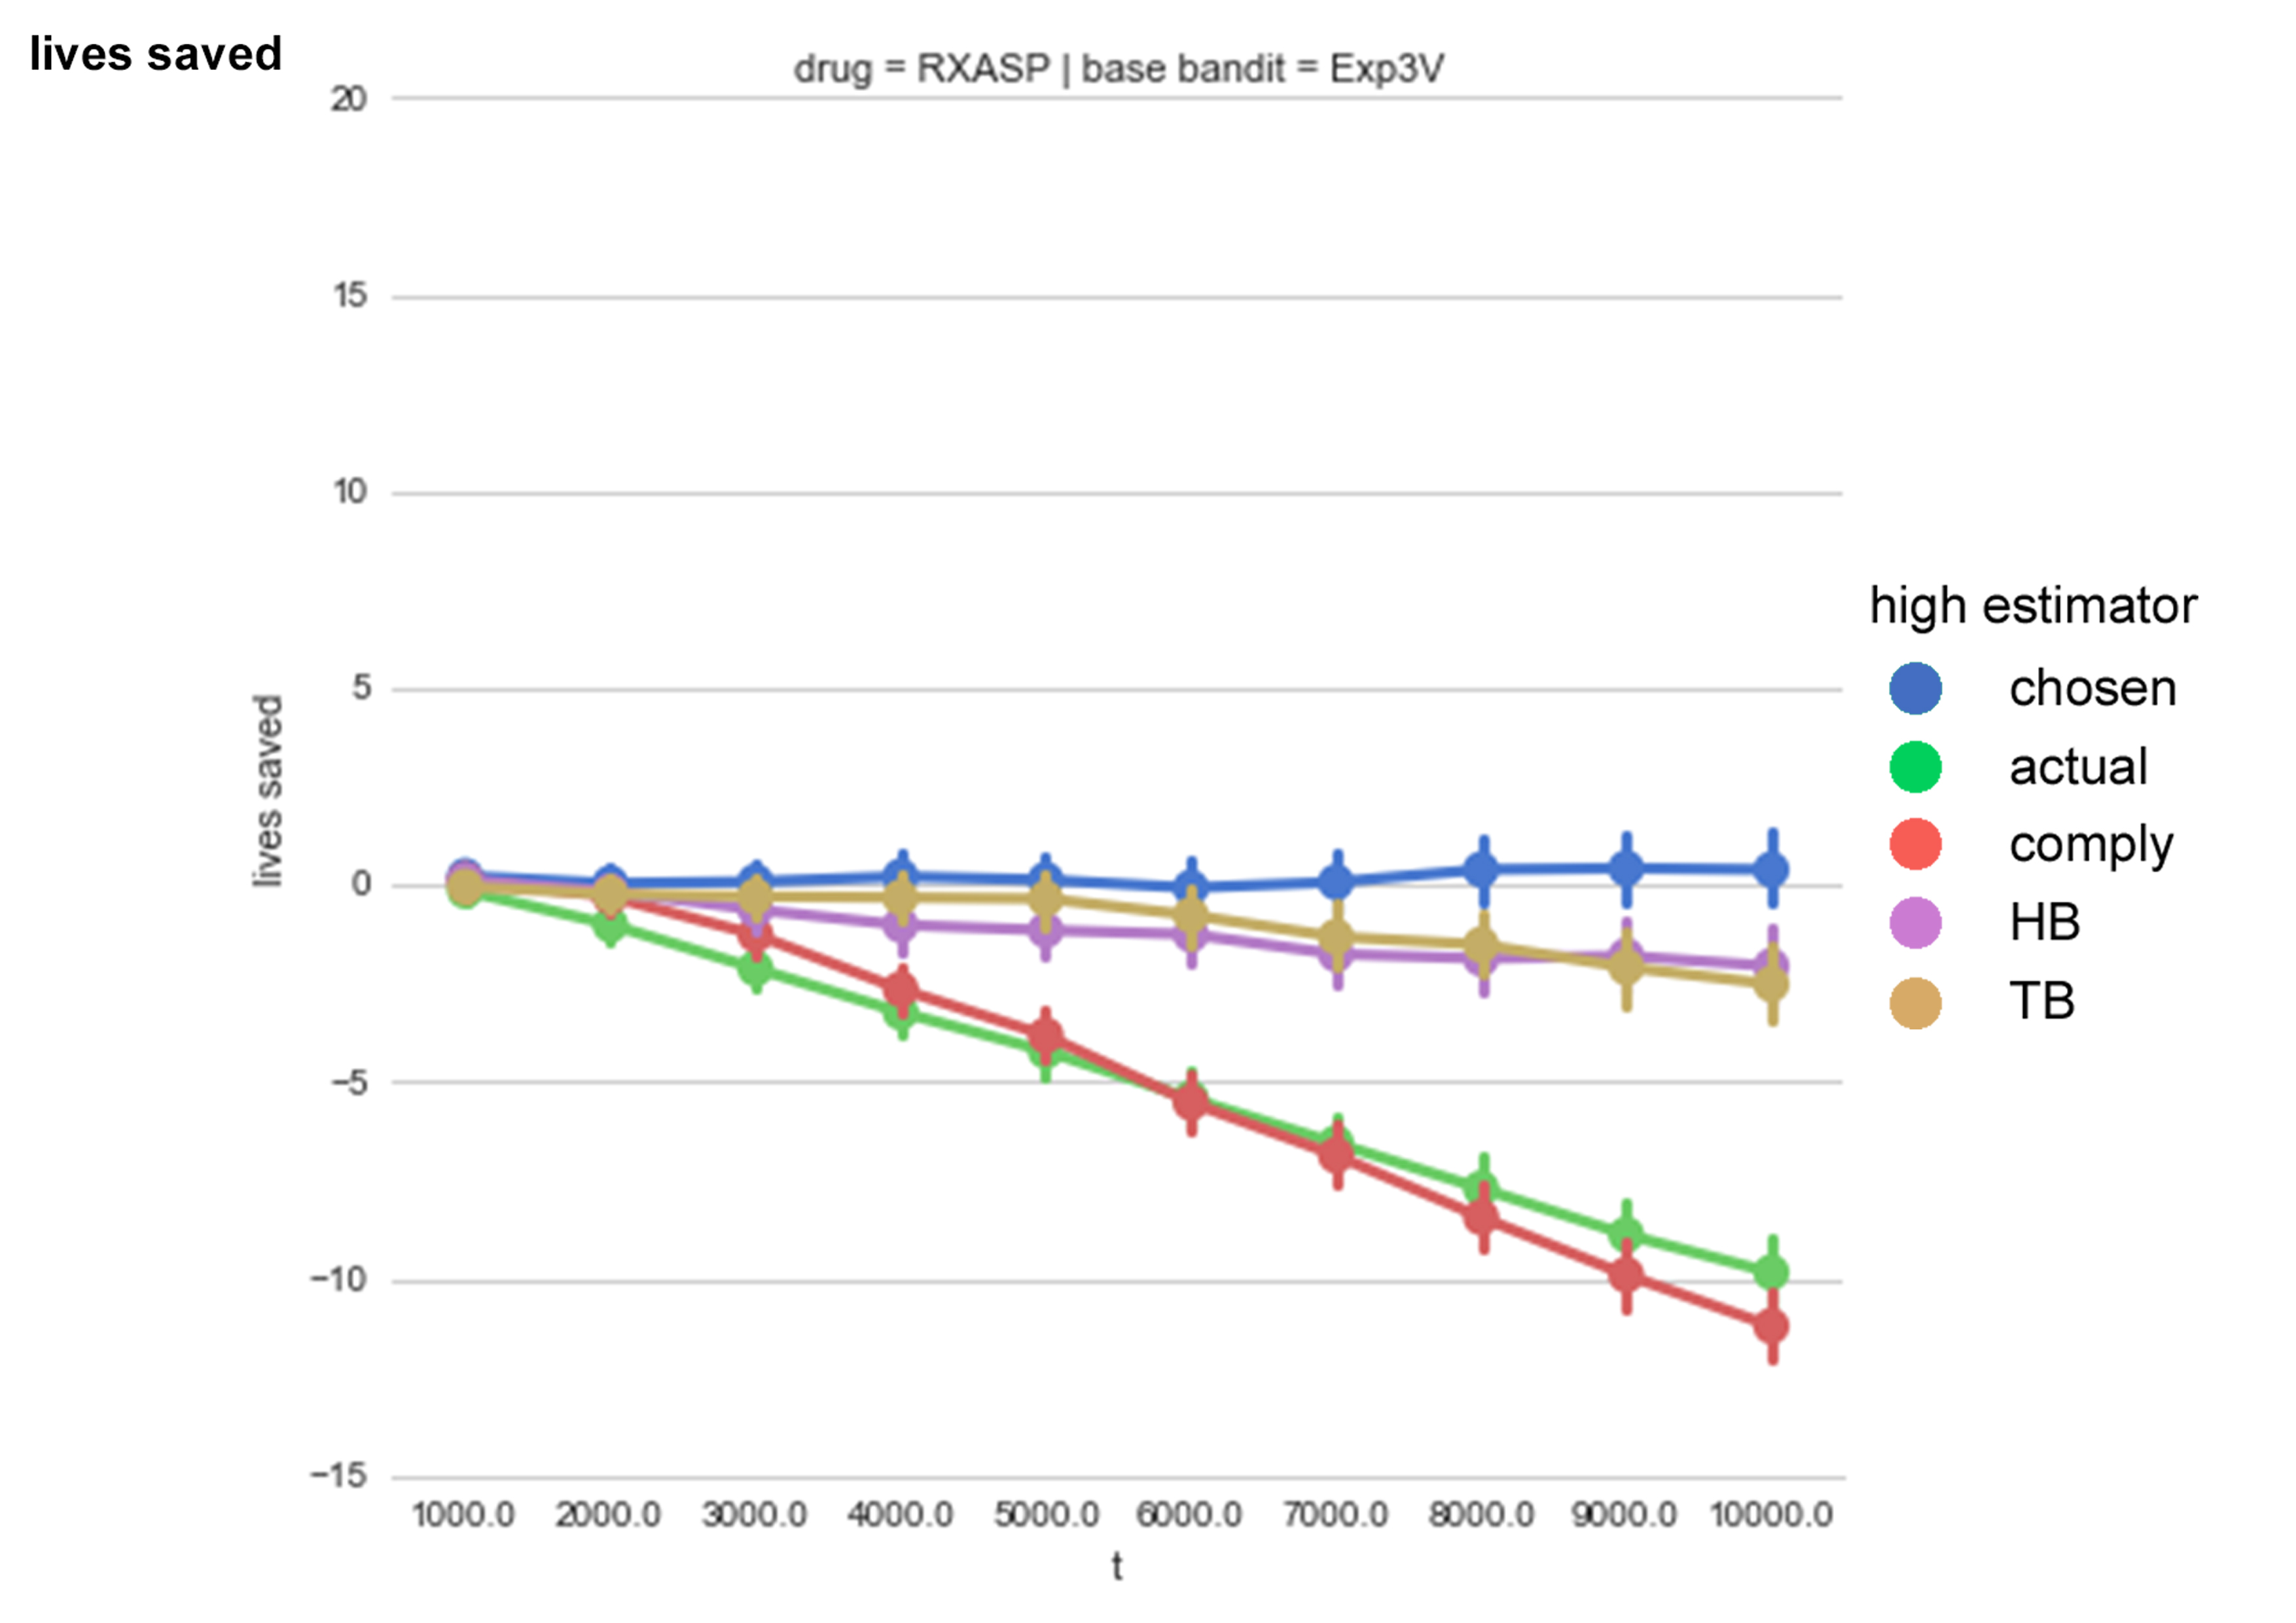
\includegraphics[width=1\columnwidth]{bandit/figs/fig1-1.jpg}
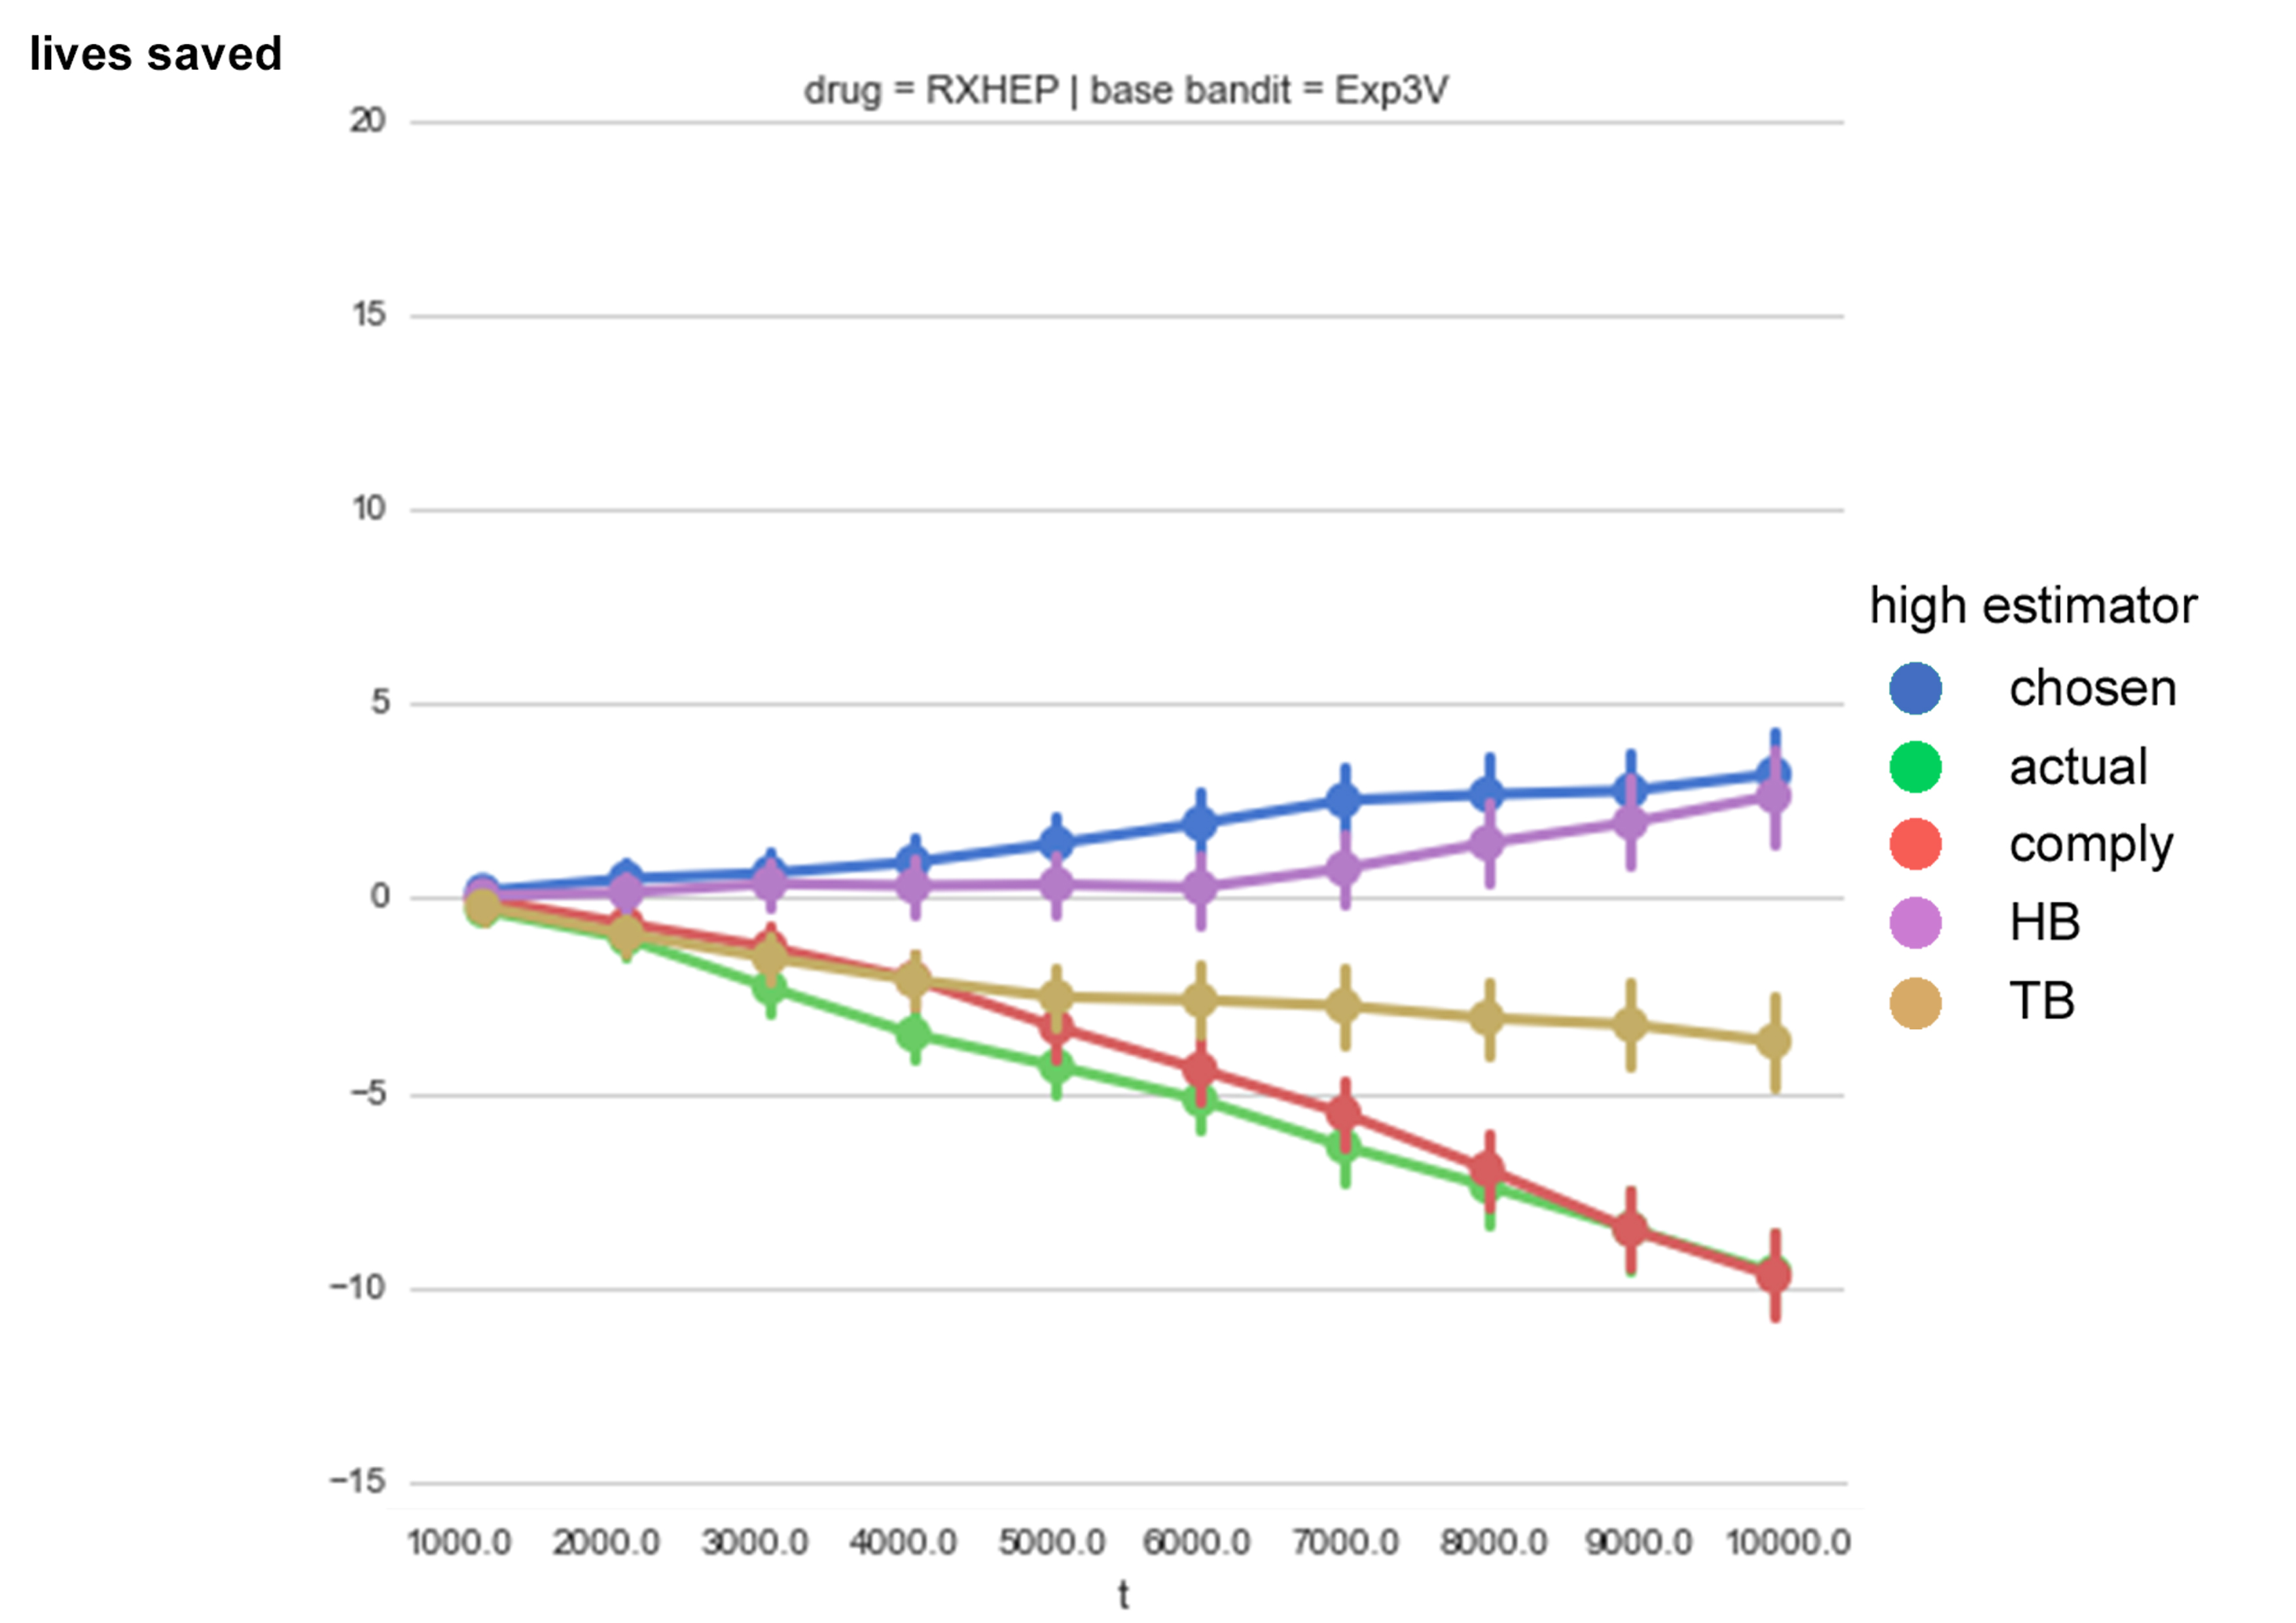
\includegraphics[width=1\columnwidth]{bandit/figs/fig1-2.jpg}
\caption{\textbf{14 Day survivals:} average lives saved over uniform random policy per 10,000 patients in 10,000 simulated trials of Aspirin and Heparin, with Exp3 as the base bandit.}
\end{center}
\end{figure} 
\begin{figure}
\begin{center}
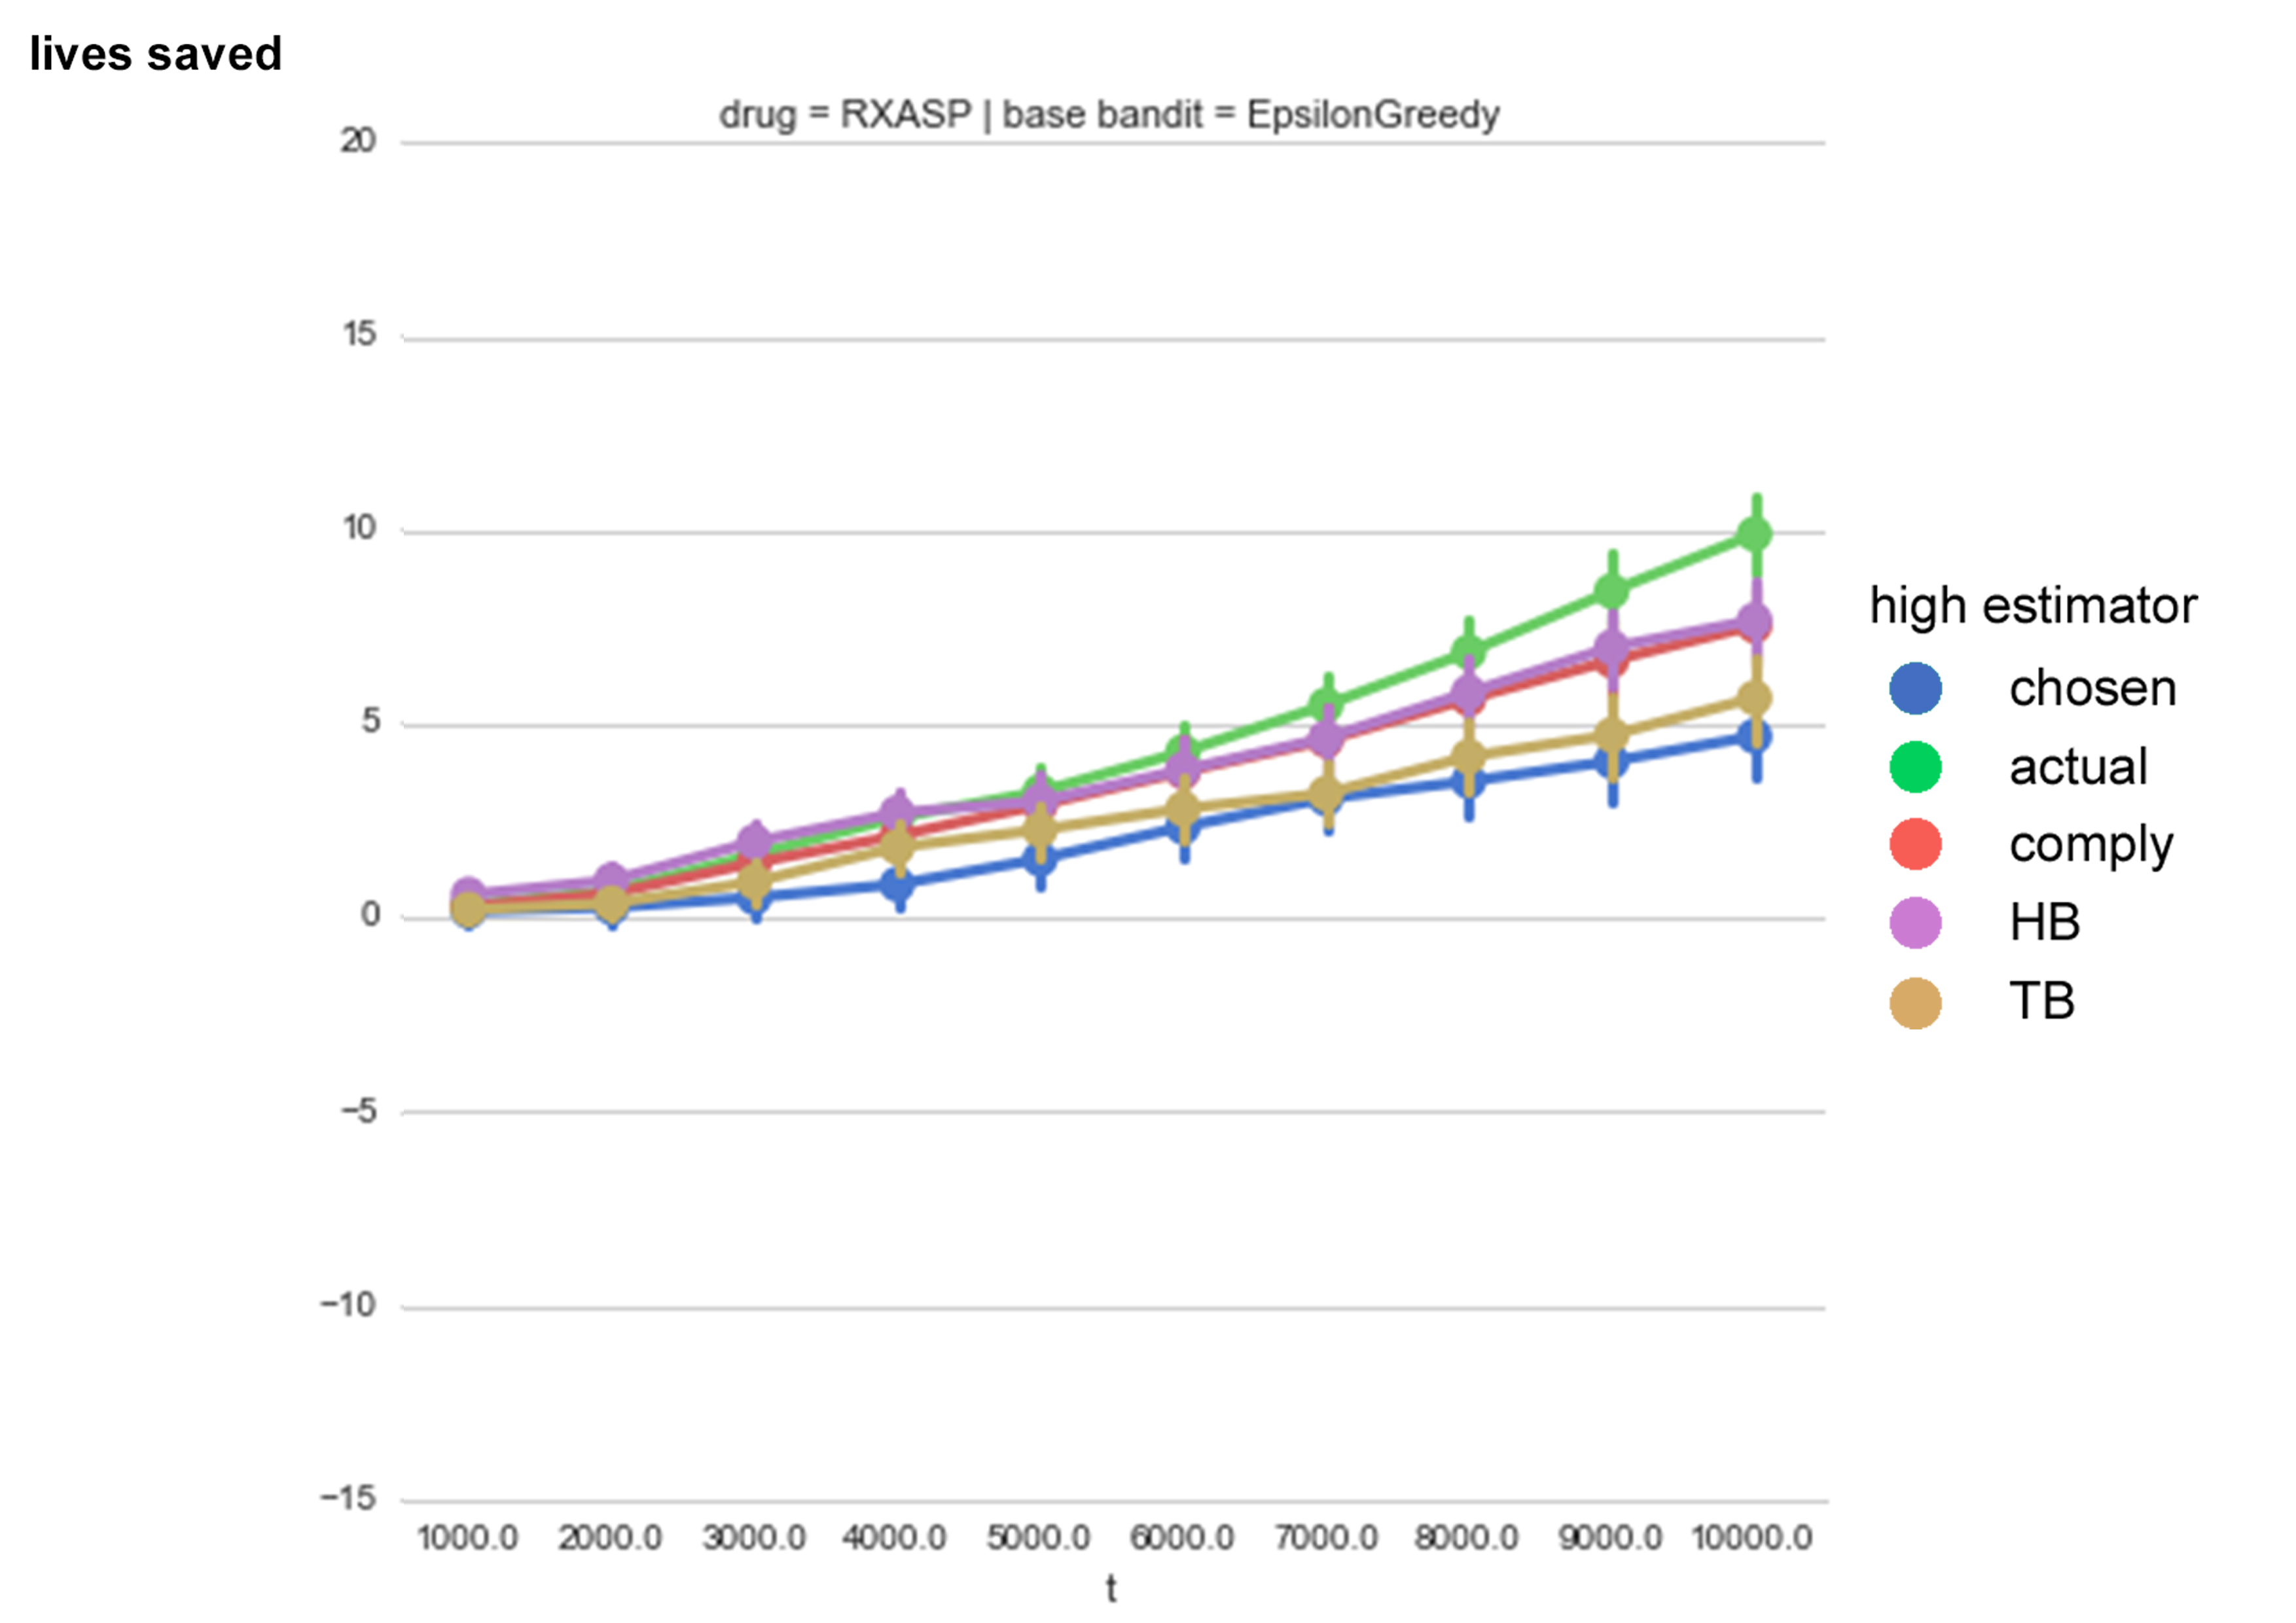
\includegraphics[width=1\columnwidth]{bandit/figs/fig1-3.jpg}
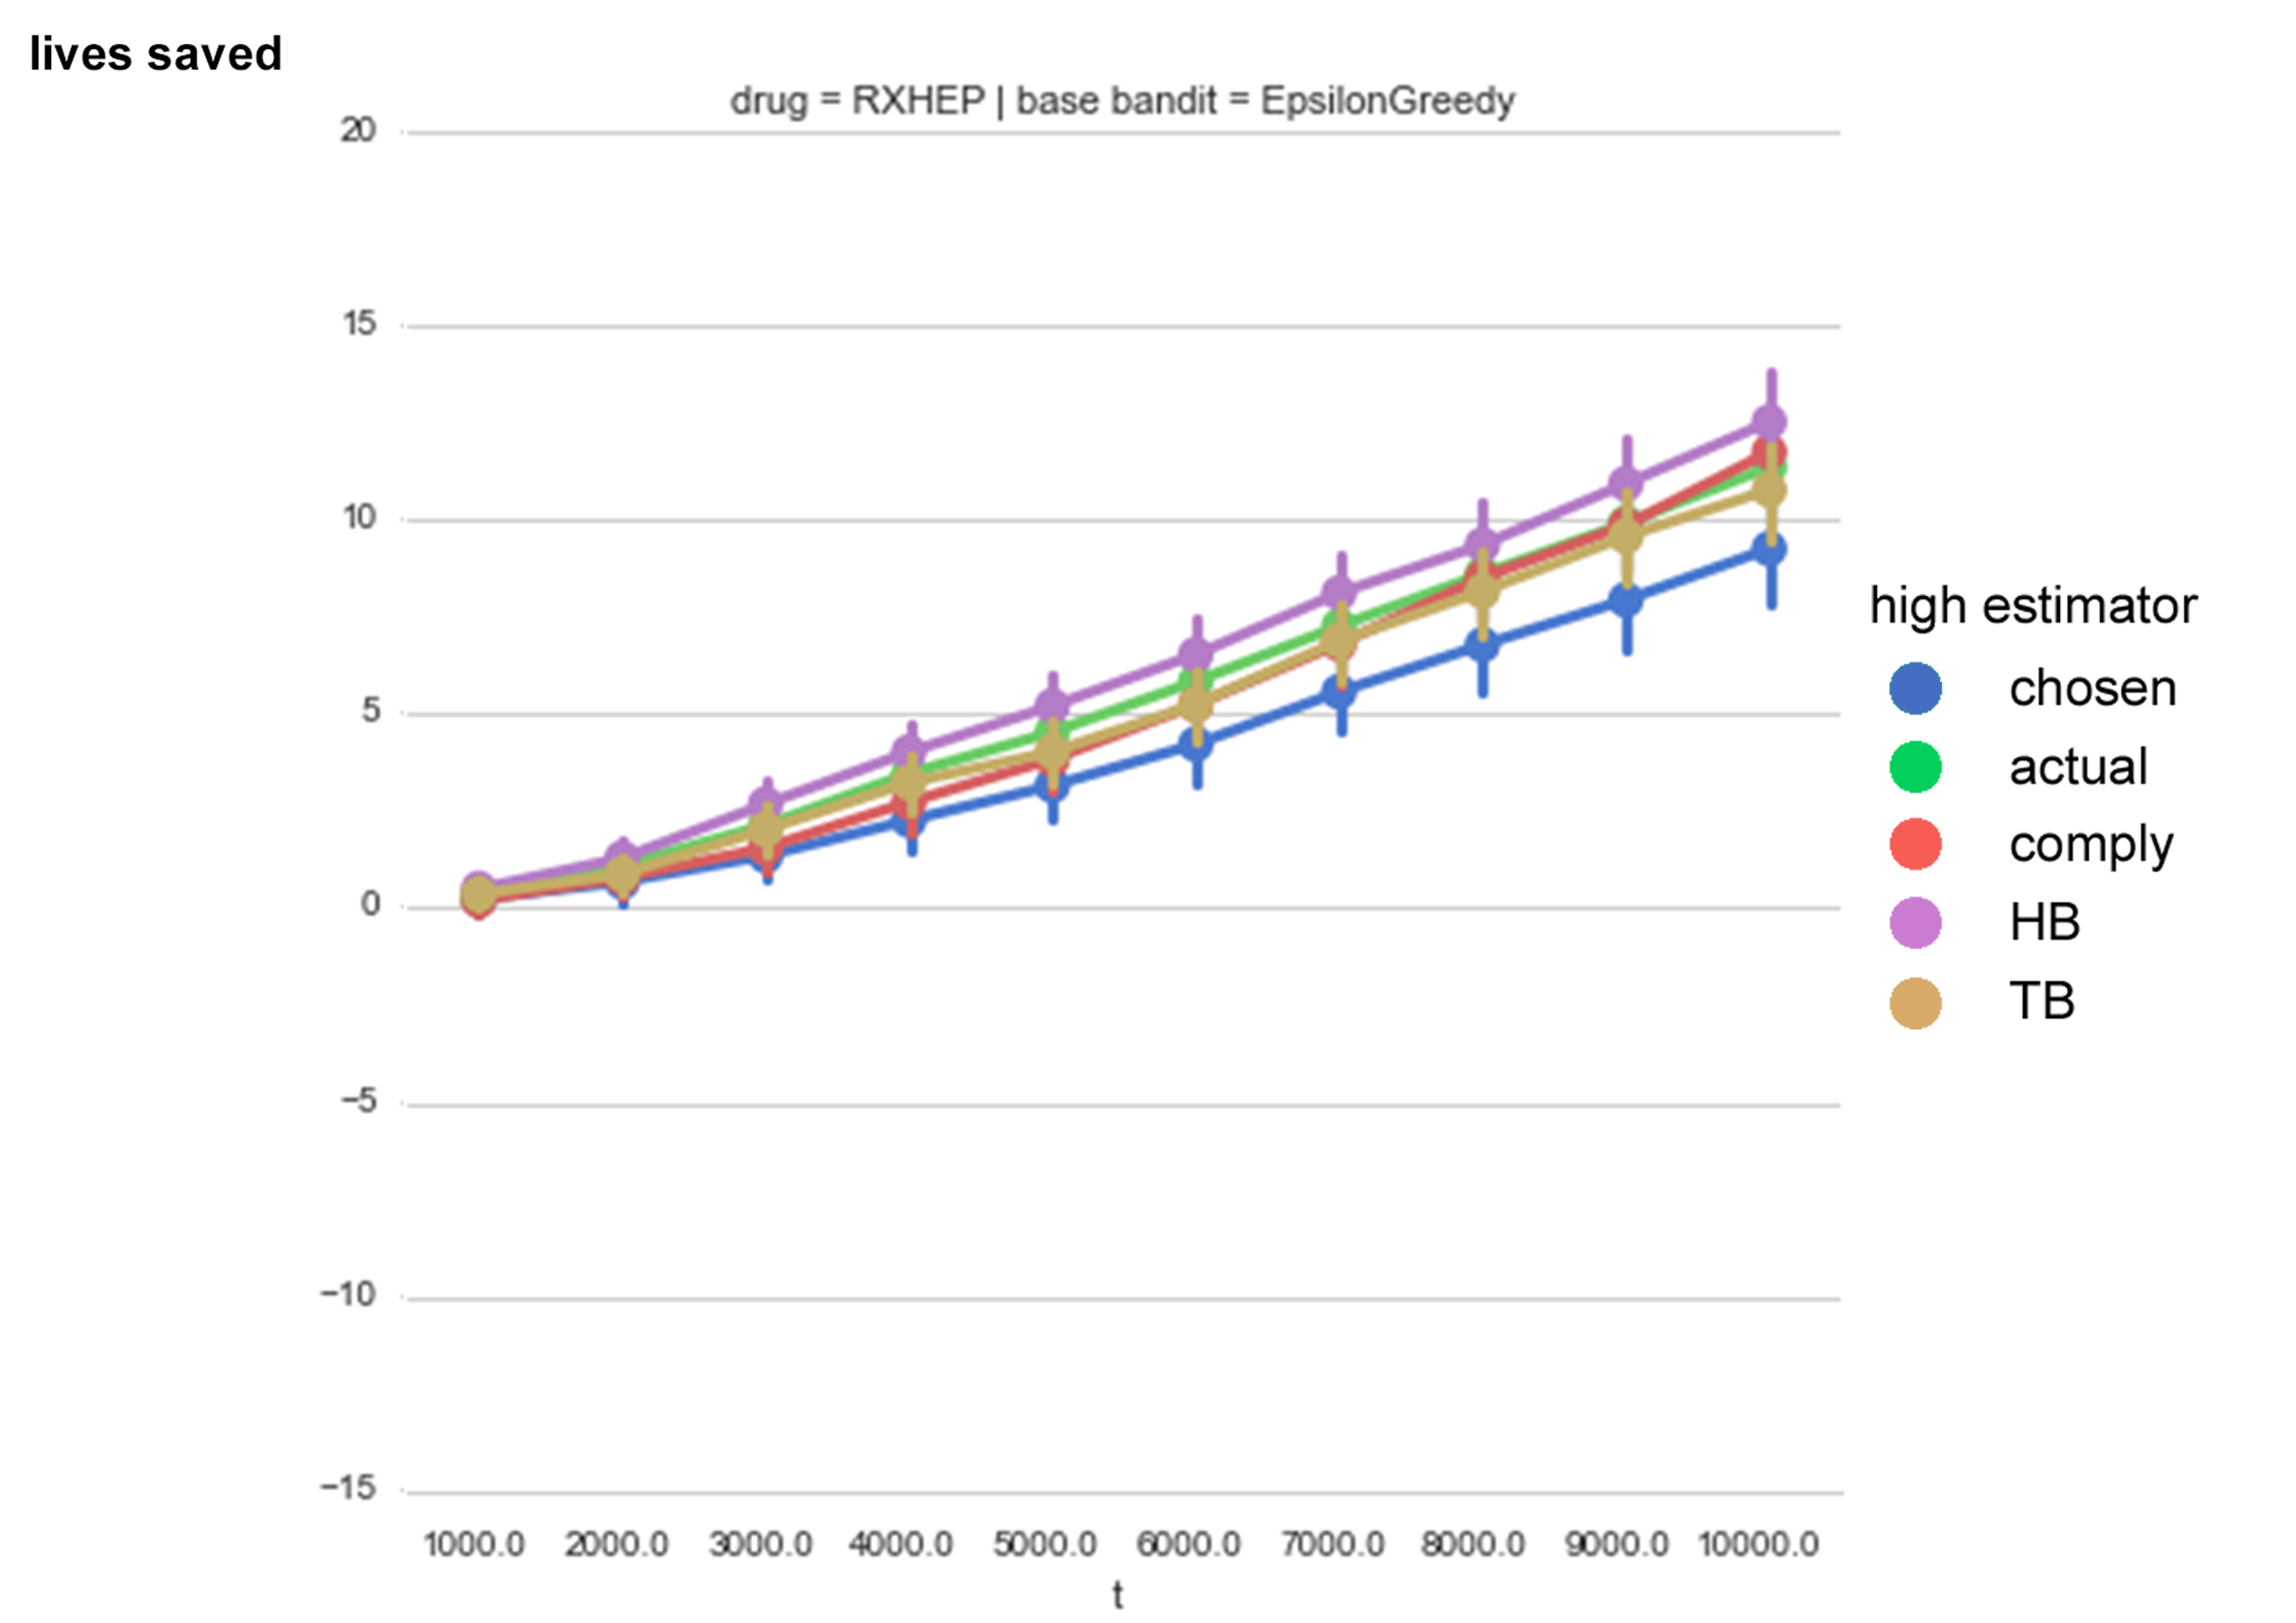
\includegraphics[width=1\columnwidth]{bandit/figs/fig1-4.jpg}
\caption{\textbf{14 Day survivals:} average lives saved over uniform random policy per 10,000 patients in 10,000 simulated trials of Aspirin and Heparin, with Epsilon Greedy as the base bandit.}
\end{center}
\end{figure} 
\begin{figure}
\begin{center}
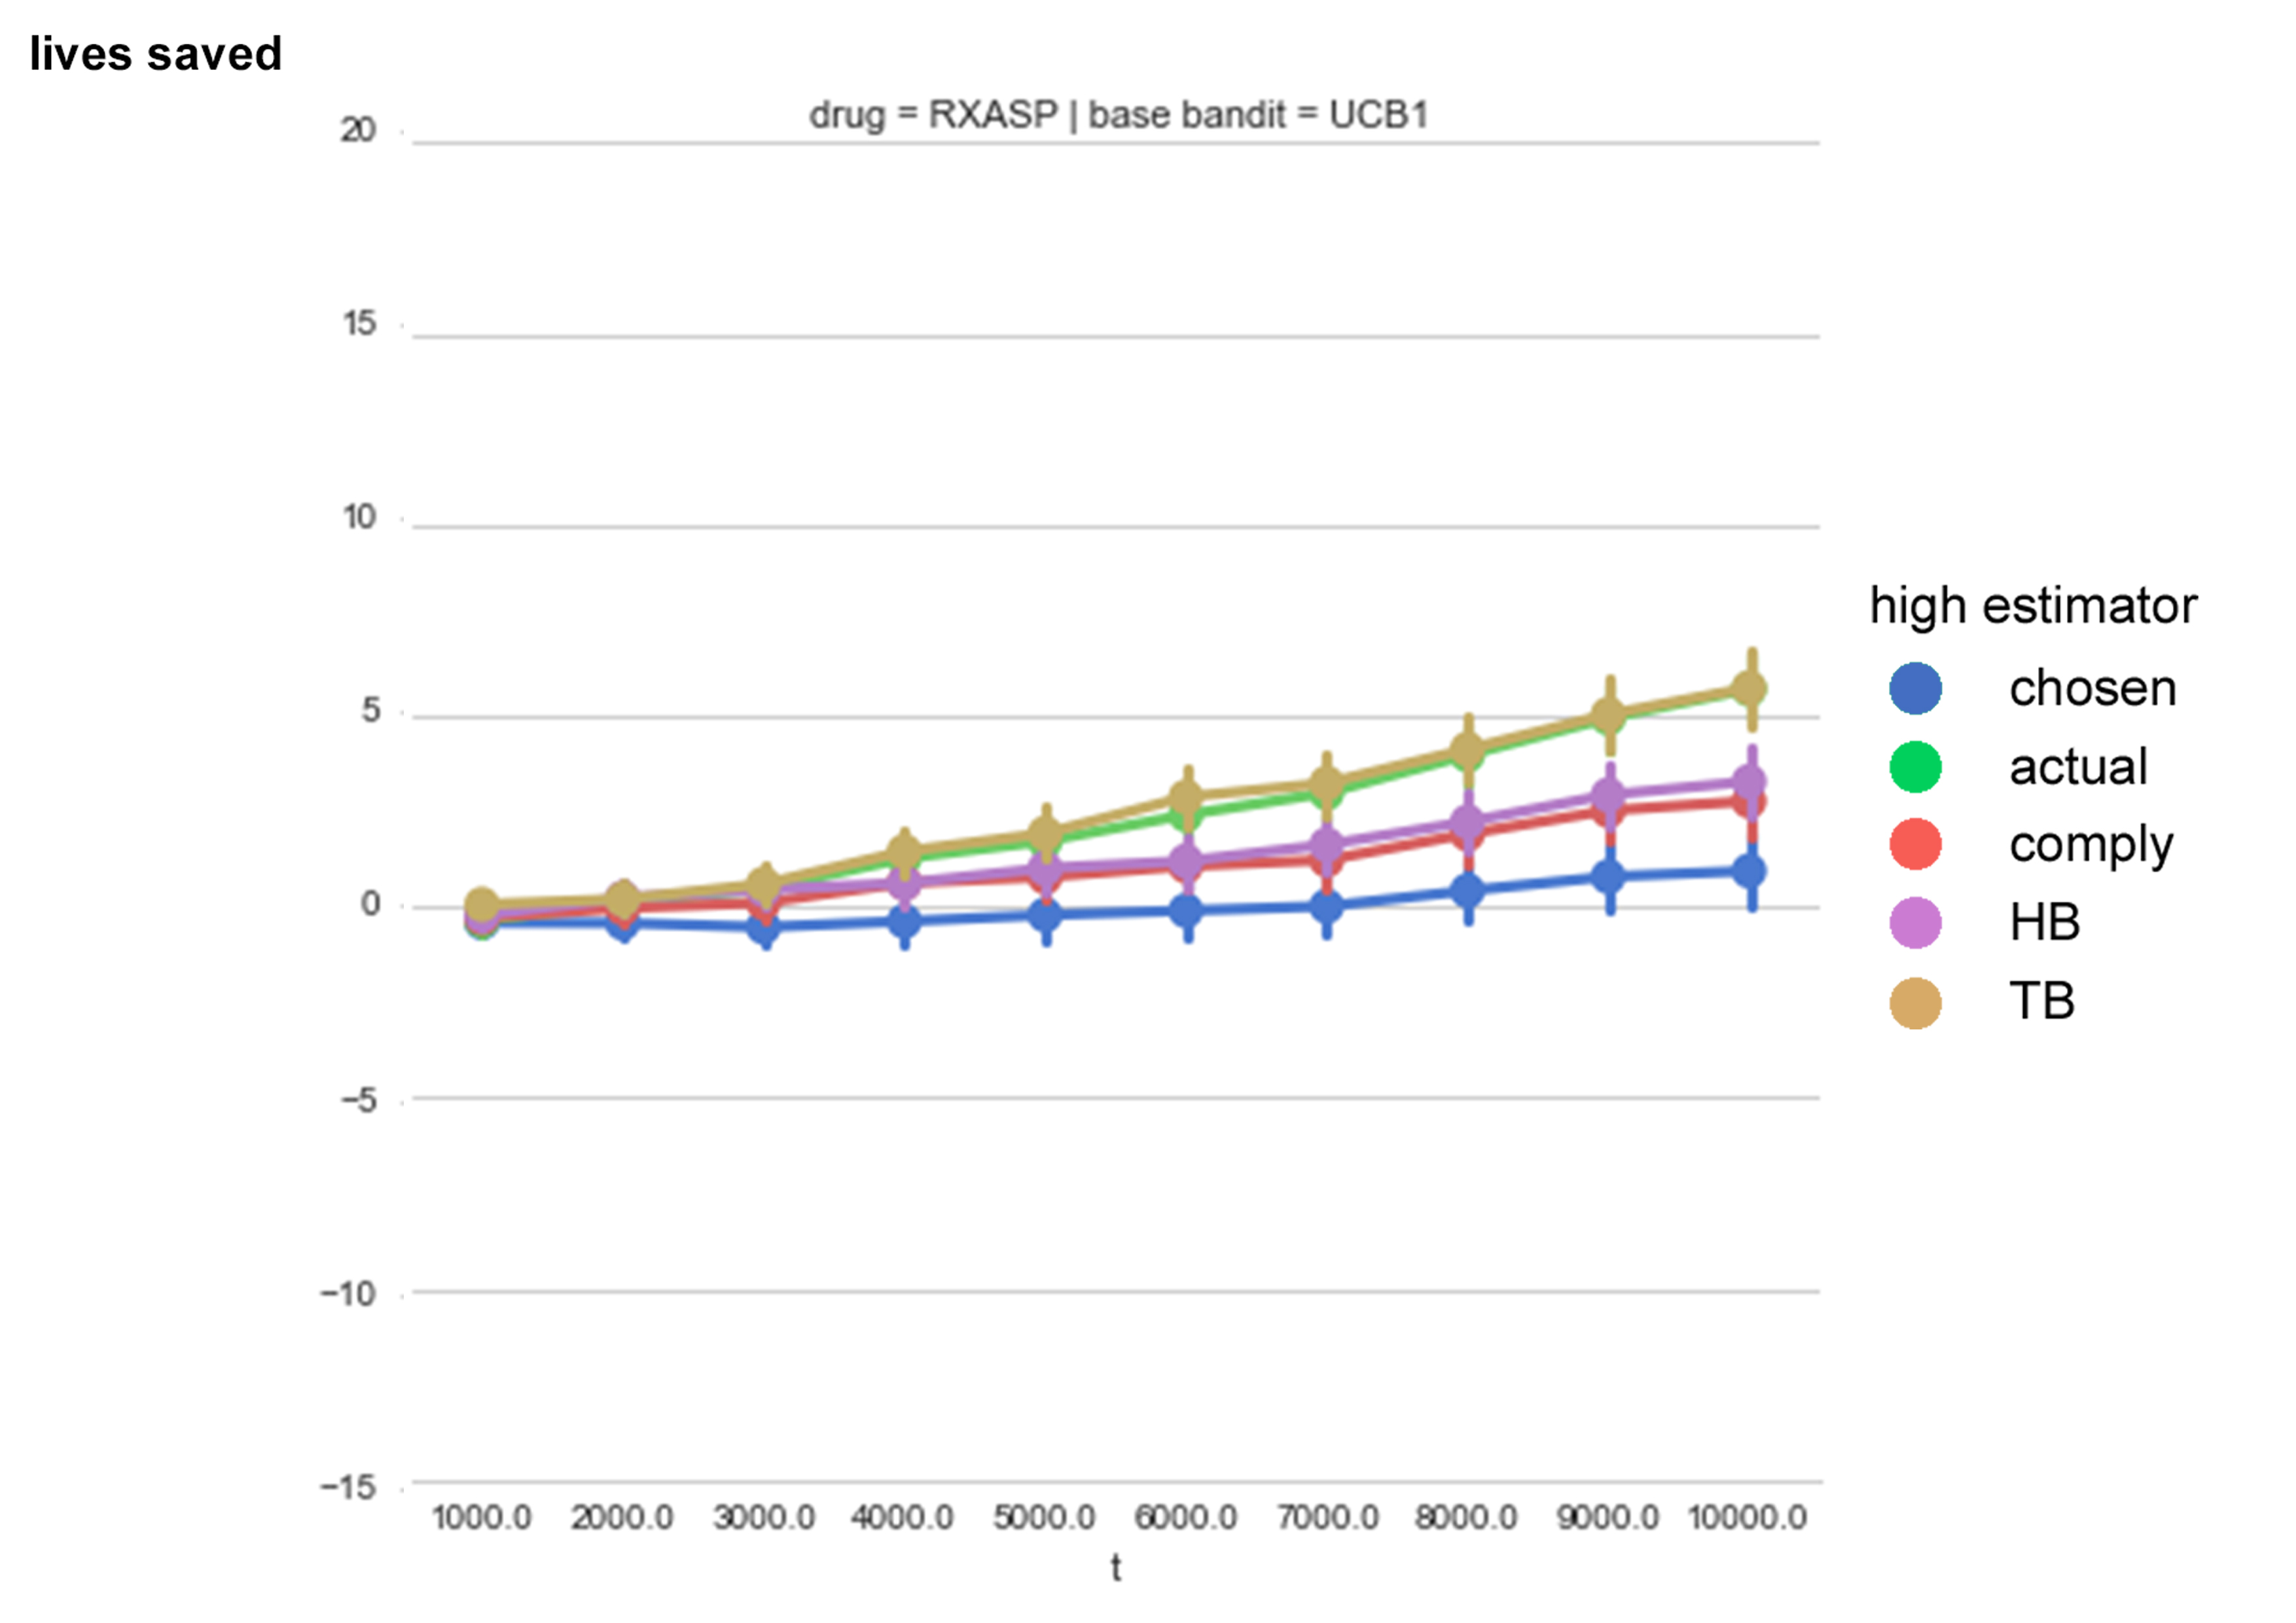
\includegraphics[width=1\columnwidth]{bandit/figs/fig1-5.jpg}
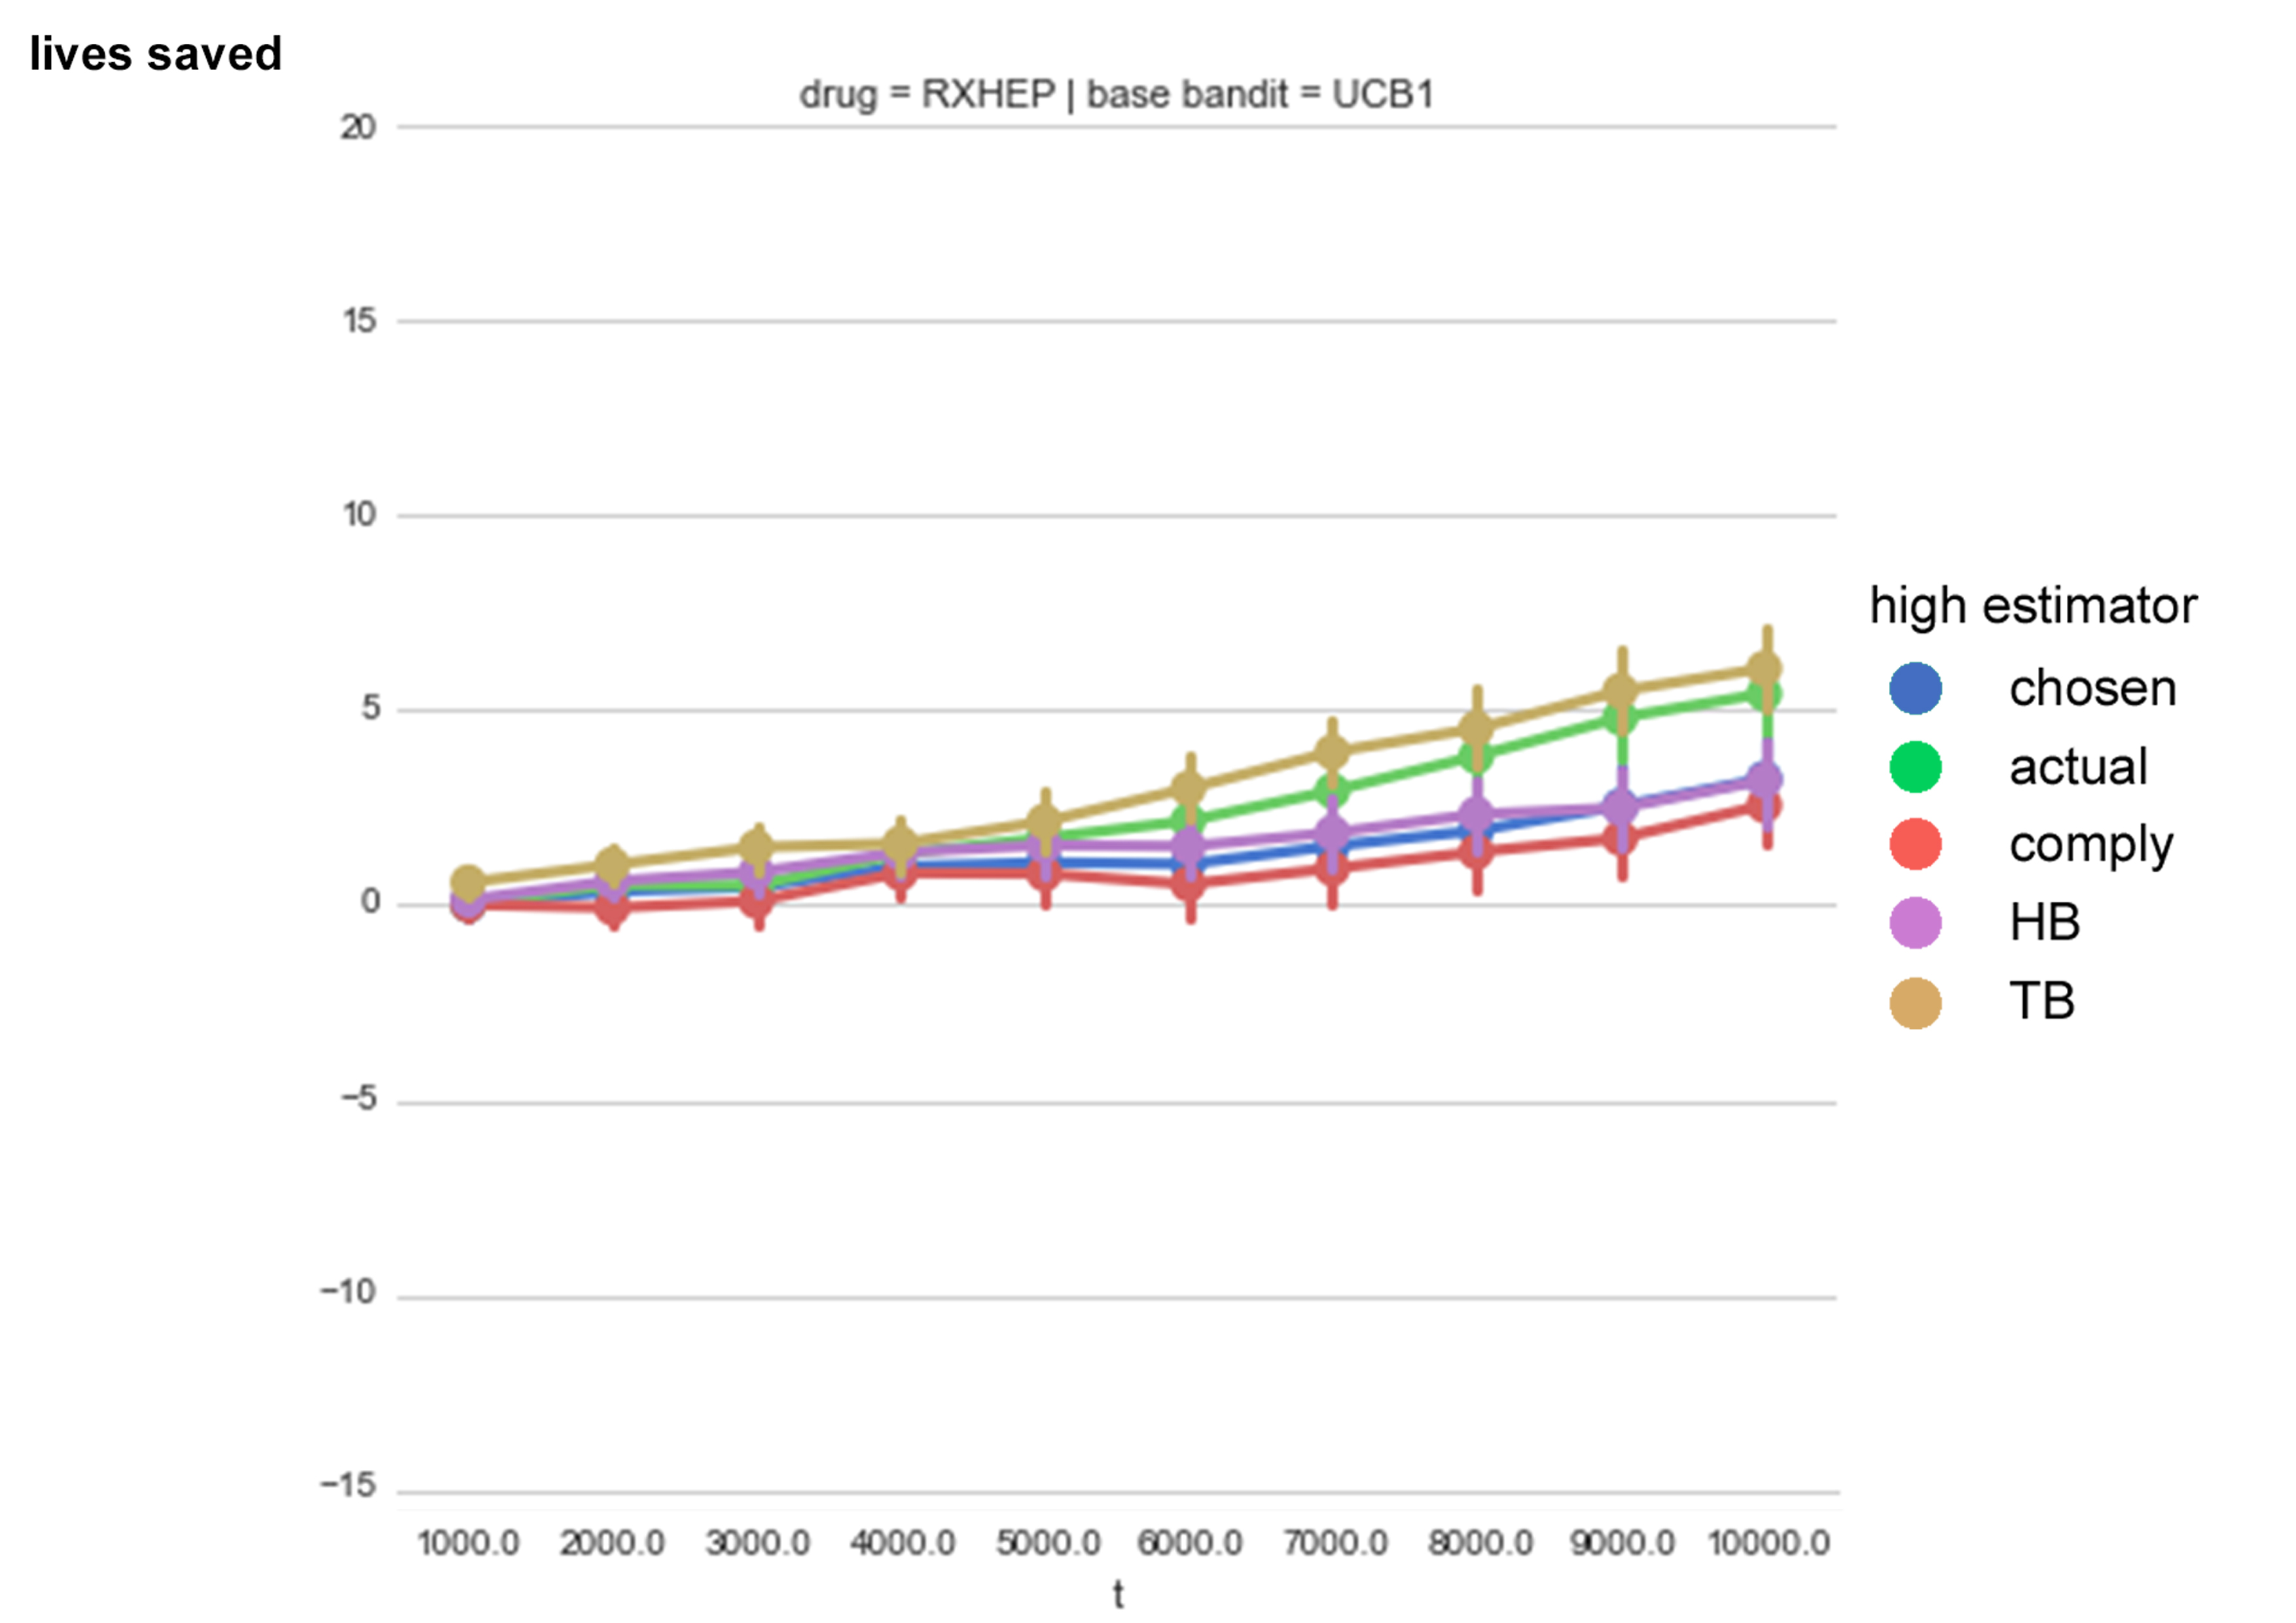
\includegraphics[width=1\columnwidth]{bandit/figs/fig1-6.jpg}
\caption{\textbf{14 Day survivals:} average lives saved over uniform random policy per 10,000 patients in 10,000 simulated trials of Aspirin and Heparin, with UCB1 as the base bandit.}
\end{center}
\end{figure} 
\begin{figure}
\begin{center}
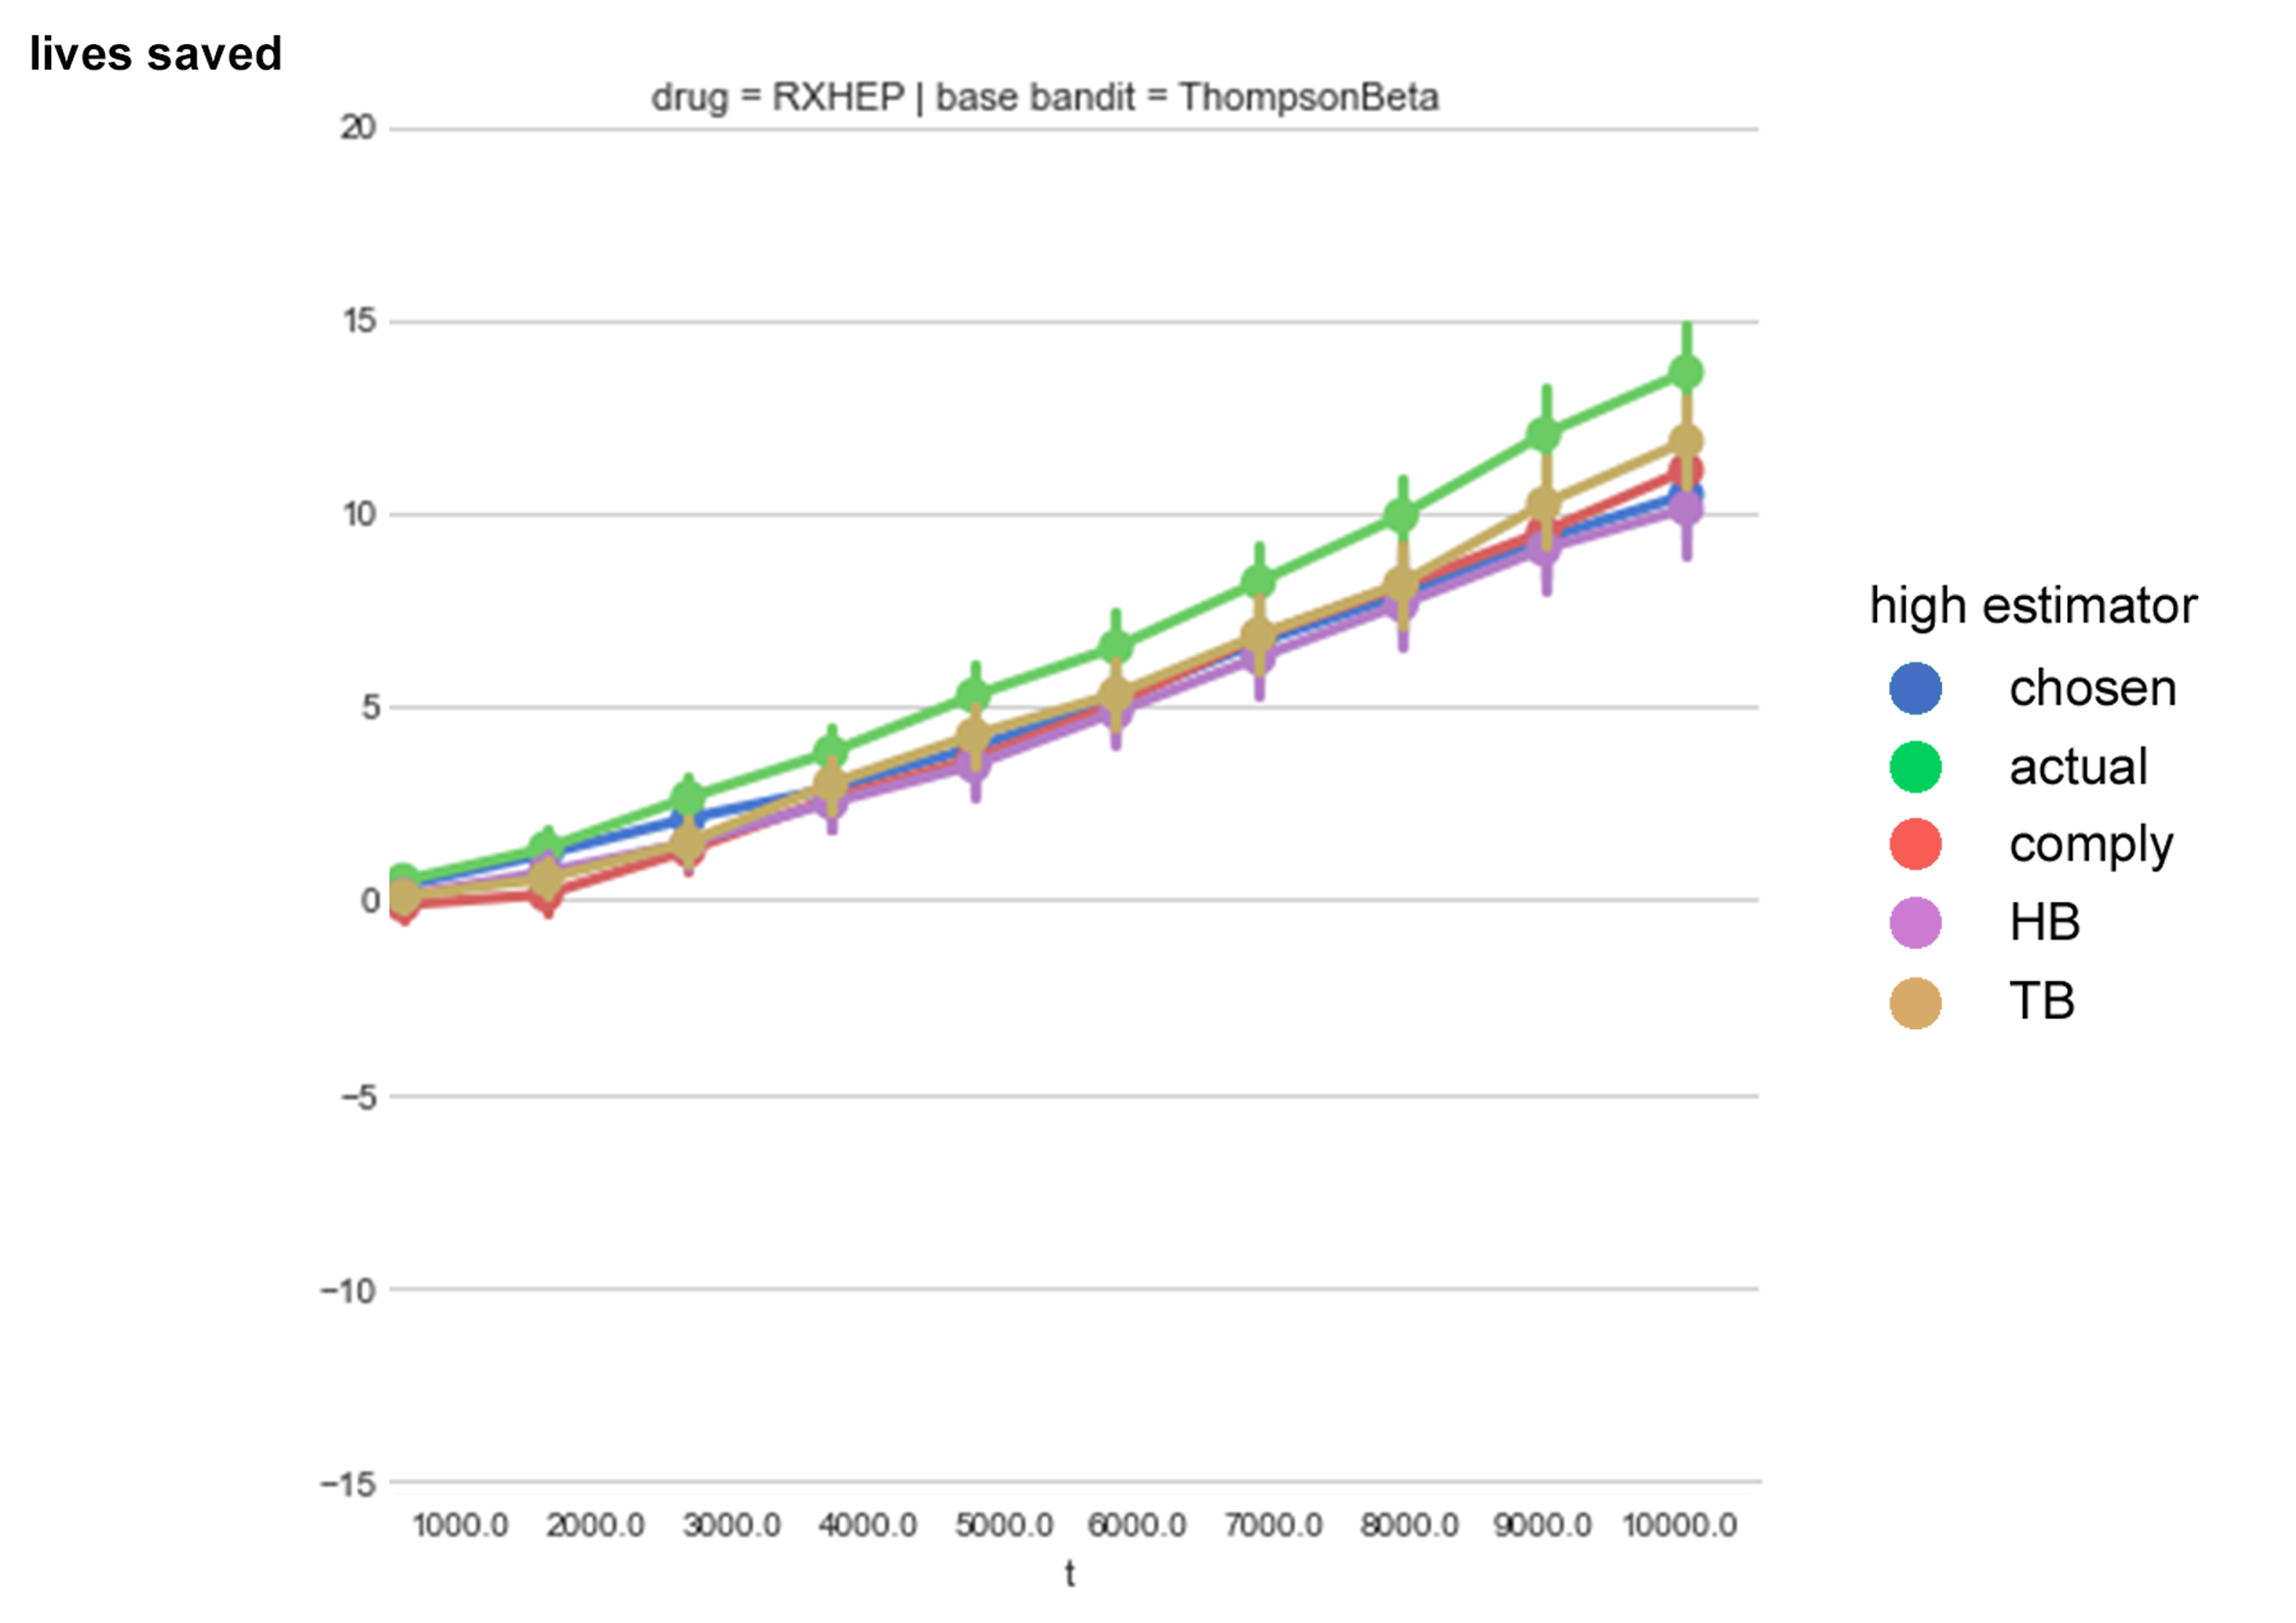
\includegraphics[width=1\columnwidth]{bandit/figs/fig1-7.jpg}
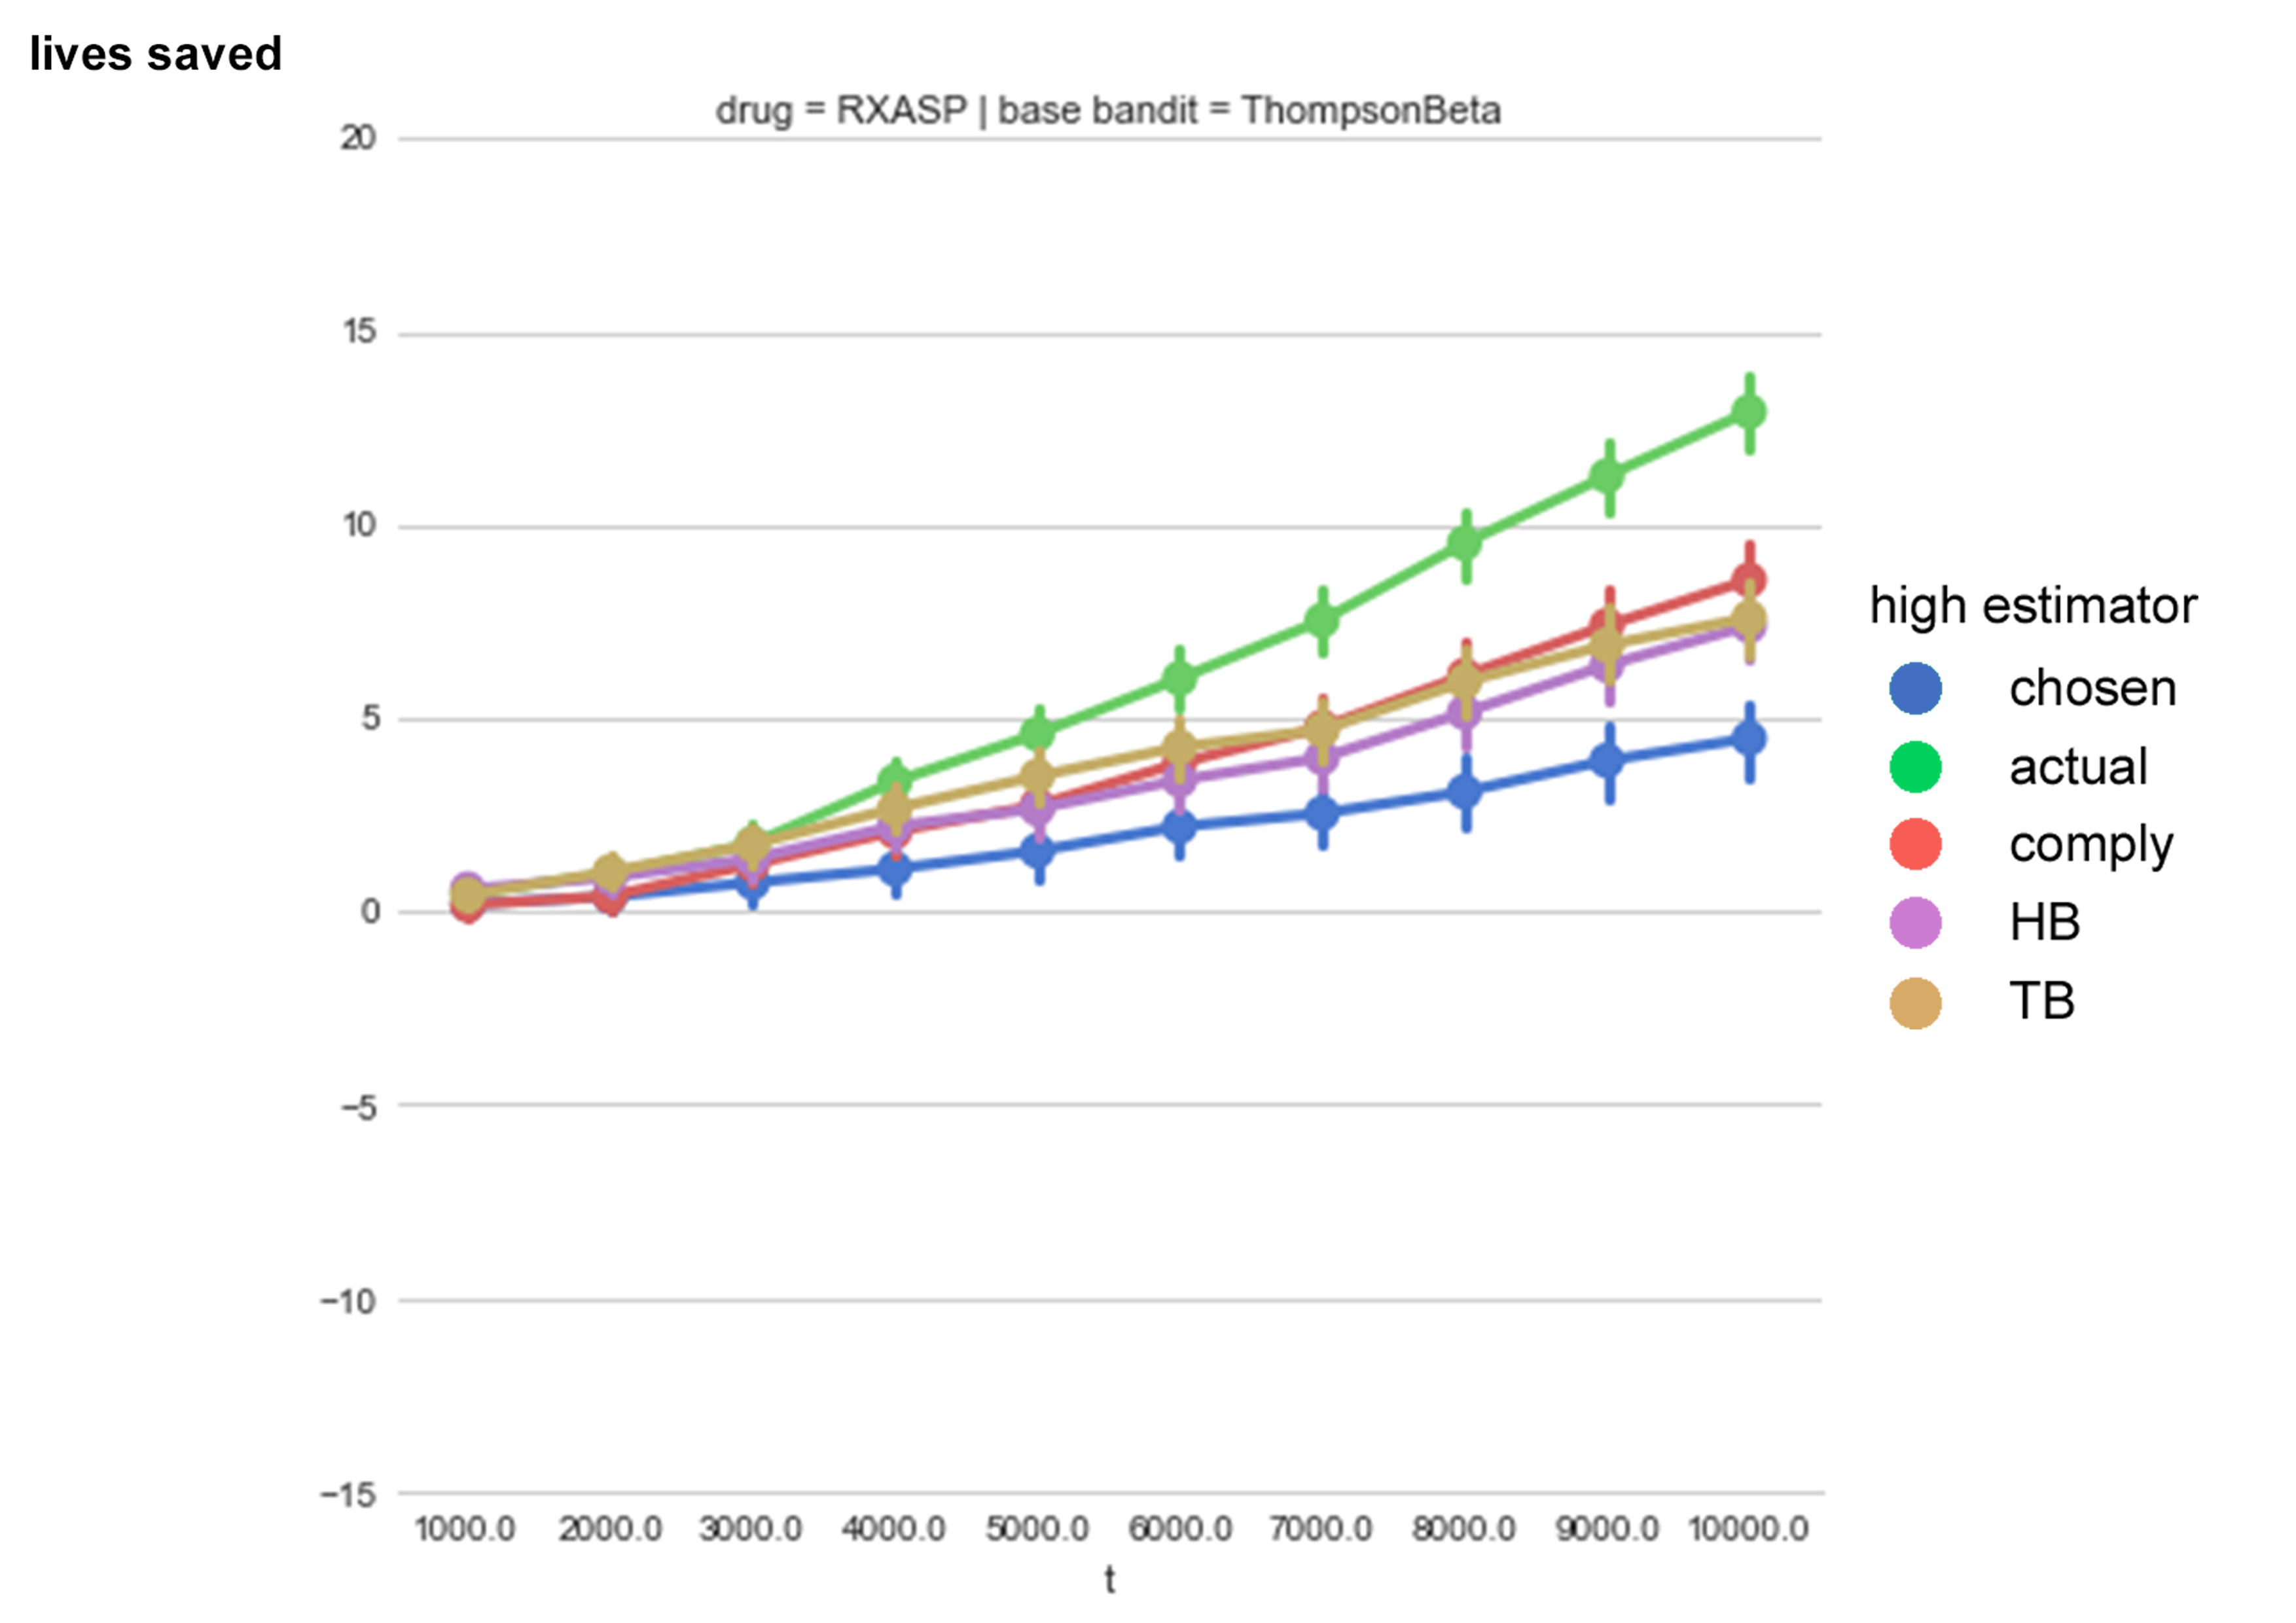
\includegraphics[width=1\columnwidth]{bandit/figs/fig1-8.jpg}
\caption{\textbf{14 Day survivals:} average lives saved over uniform random policy per 10,000 patients in 10,000 simulated trials of Aspirin and Heparin, with Thompson sampling as the base bandit.}
\label{fig1a}
\end{center}
\end{figure} 

%\begin{figure}
%\begin{center}
	%\textwidth, angle=90
%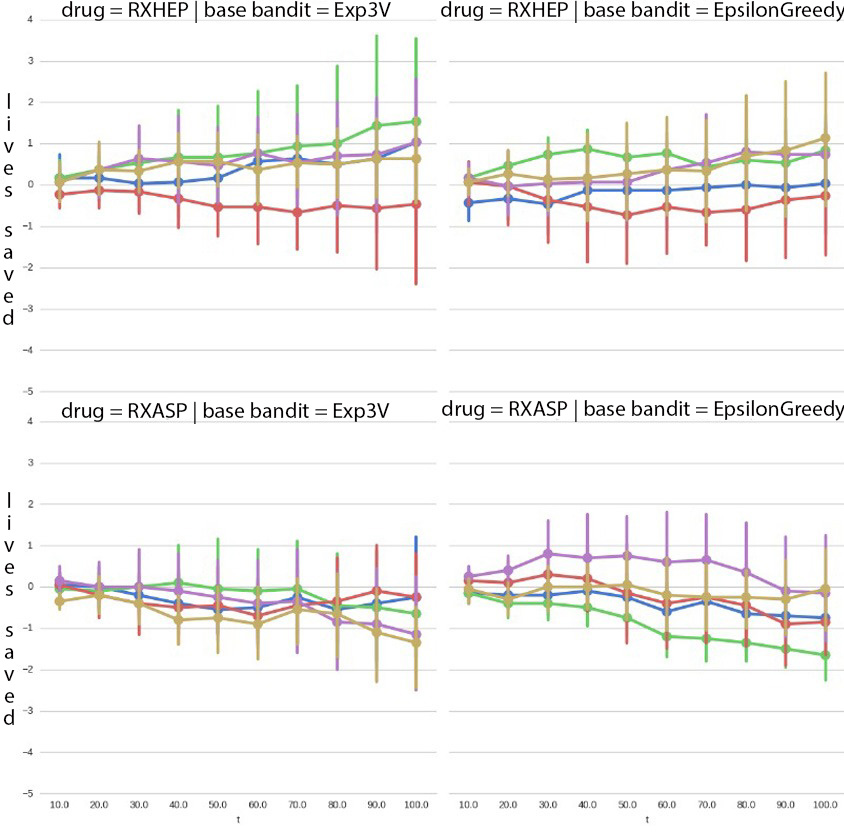
\includegraphics[width=1\columnwidth]{bandit/figs/fig1b.jpg}
%\caption{\textbf{14 Day survivals:} average lives saved over uniform random policy per 10,000 patients in 10,000 simulated trials of Aspirin and Heparin individually.}
%\label{fig1b}
%\end{center}
%\end{figure} 


We simulated 10,000 patients per run, which allowed us to not oversample the data in any single simulation. A total of 2000 runs were performed, all algorithms were tested against the same draw of the run to minimize unnecessary sampling variation. 

The \texttt{EXP3} gamma parameter was set ahead of time to 0.085, a choice determined by the regret-bounds for $T=10000$ and $K=2$ or $K=3$. Epsilon-Greedy used a standard annealing schedule. No data dependent parameter tuning was used.
The simulation was carried out by creating a ``counter-factual patient'': one patient was sampled i.i.d. from each treatment and control groups in the clinical trial. If the algorithm selected the treatment, it received the reward and observed the action taken by the subject sampled form the treatment group, and vice versa for the control.


Empirically, \texttt{TB} achieved a surplus of 8.9 extra survivals (that is, human lives) with 95\% confidence interval $[8.1,9.7]$, relative to the randomized baseline.
\texttt{HB} with \texttt{Epsilon Greedy} as the base algorithm achieved a surplus of 9.2 (CI: $[8.3,10.0]$)
In contrast, the best performing strategy that was not compliance aware was Thompson sampling, which yielded 7.9 extra survivals (CI: $[7.2,8.7]$). 
%TODO bob wants you to interpret results: Tell the reader what one can conclude (and perhaps what one can not conclude) from the experimental results.
% The data in the IST is for a large worldwide trial for a widely available moderate effect intervention ( ) 

The gains were largely concentrated in the Aspirin trial, which is consistent with the lack of benefits or severe ill effects found in the original study \cite{ist:97} for heparin, and with the small but beneficial effect found for aspirin. 
If the underlying treatment has no positive or negative effect, side-information after the fact alone cannot be helpful.
Note that \actual, and to a lesser extent \comply, performed better than either \chosen\, or the hybrid algorithms. However, these are problematic to use directly since no guarantees apply to their worst case performance. The performance of the hybrids benefits from the information encoded in \actual\, and \comply\, whilst keeping the guarantees of \chosen. 


A striking secondary empirical observation from the experiments is the strong interaction between the base learning algorithm and the nature of the feedback used. In particular, our naive implementation of \texttt{EXP3} performed extremely badly under both \actual\, and \comply, in both the aspirin and heparin simulations. In contrast, \texttt{EXP3} performs well when used as a top-level algorithm in \texttt{HB} in both trials, and other algorithms on the same data with the same protocol are able to learn better than \chosen, while \texttt{EXP3} does worse than random (note the \texttt{EXP3} guarantees are only for the \chosen\, protocol, so they do not apply here).
%TODO this is not a sentence i think...



\section{Synthetic Data}


To better understand the behavior of the algorithms in a more varied range of settings, we present results of simulations with synthetic data.



\subsection{Selection of treatment on unobservables}
%illustrates Example~\eqref{eg:rich}
The first simulation has two equally sized subpopulations of rich, healthy patients who always take the treatment, and poor, less healthy patients who only take the treatment if prescribed. Suppose the treatment reduces the probability for survival by 0.25. Assume that the rich patients would all do well (receive reward of 1) if they didn't take the treatment, but they all take it and so face only a 0.75 chance of survival. Poor patients who face a baseline survival of 0.75 only take the treatment if instructed, which brings their survival probability down to 0.5.

For comparison, $T$ was kept at 10,000, and we simulated the binary outcome case. We assigned half the patients to rich and half to poor randomly. Fig.~\eqref{fig:ex2} shows that the performance of \actual\, and \comply\, is much worse than \chosen\, and the hybrid algorithms. Results are for 100 samples.
%TODO discuss results
%\input{tables/ex2}

 A lack of useful information about underlying treatments in the compliance behaviour, their misleading nature, drives high regret in naive strategies for using compliance information. 
%\input{figs/ex2}


\begin{figure}
	\label{fig:ex2}
	\centering	
	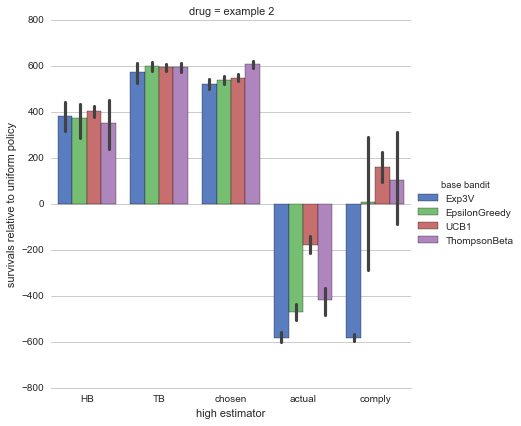
\includegraphics[width=1\columnwidth]{bandit/figs/ex2.png}\hspace{1cm}
		\caption{The naive ways of incorporating compliance, actual and comply based policies, perform poorly in this example, due to the non-compliance being in the opposing direction to the better choice.}
\end{figure}

%\begin{figure}
%	\centering	
	
%	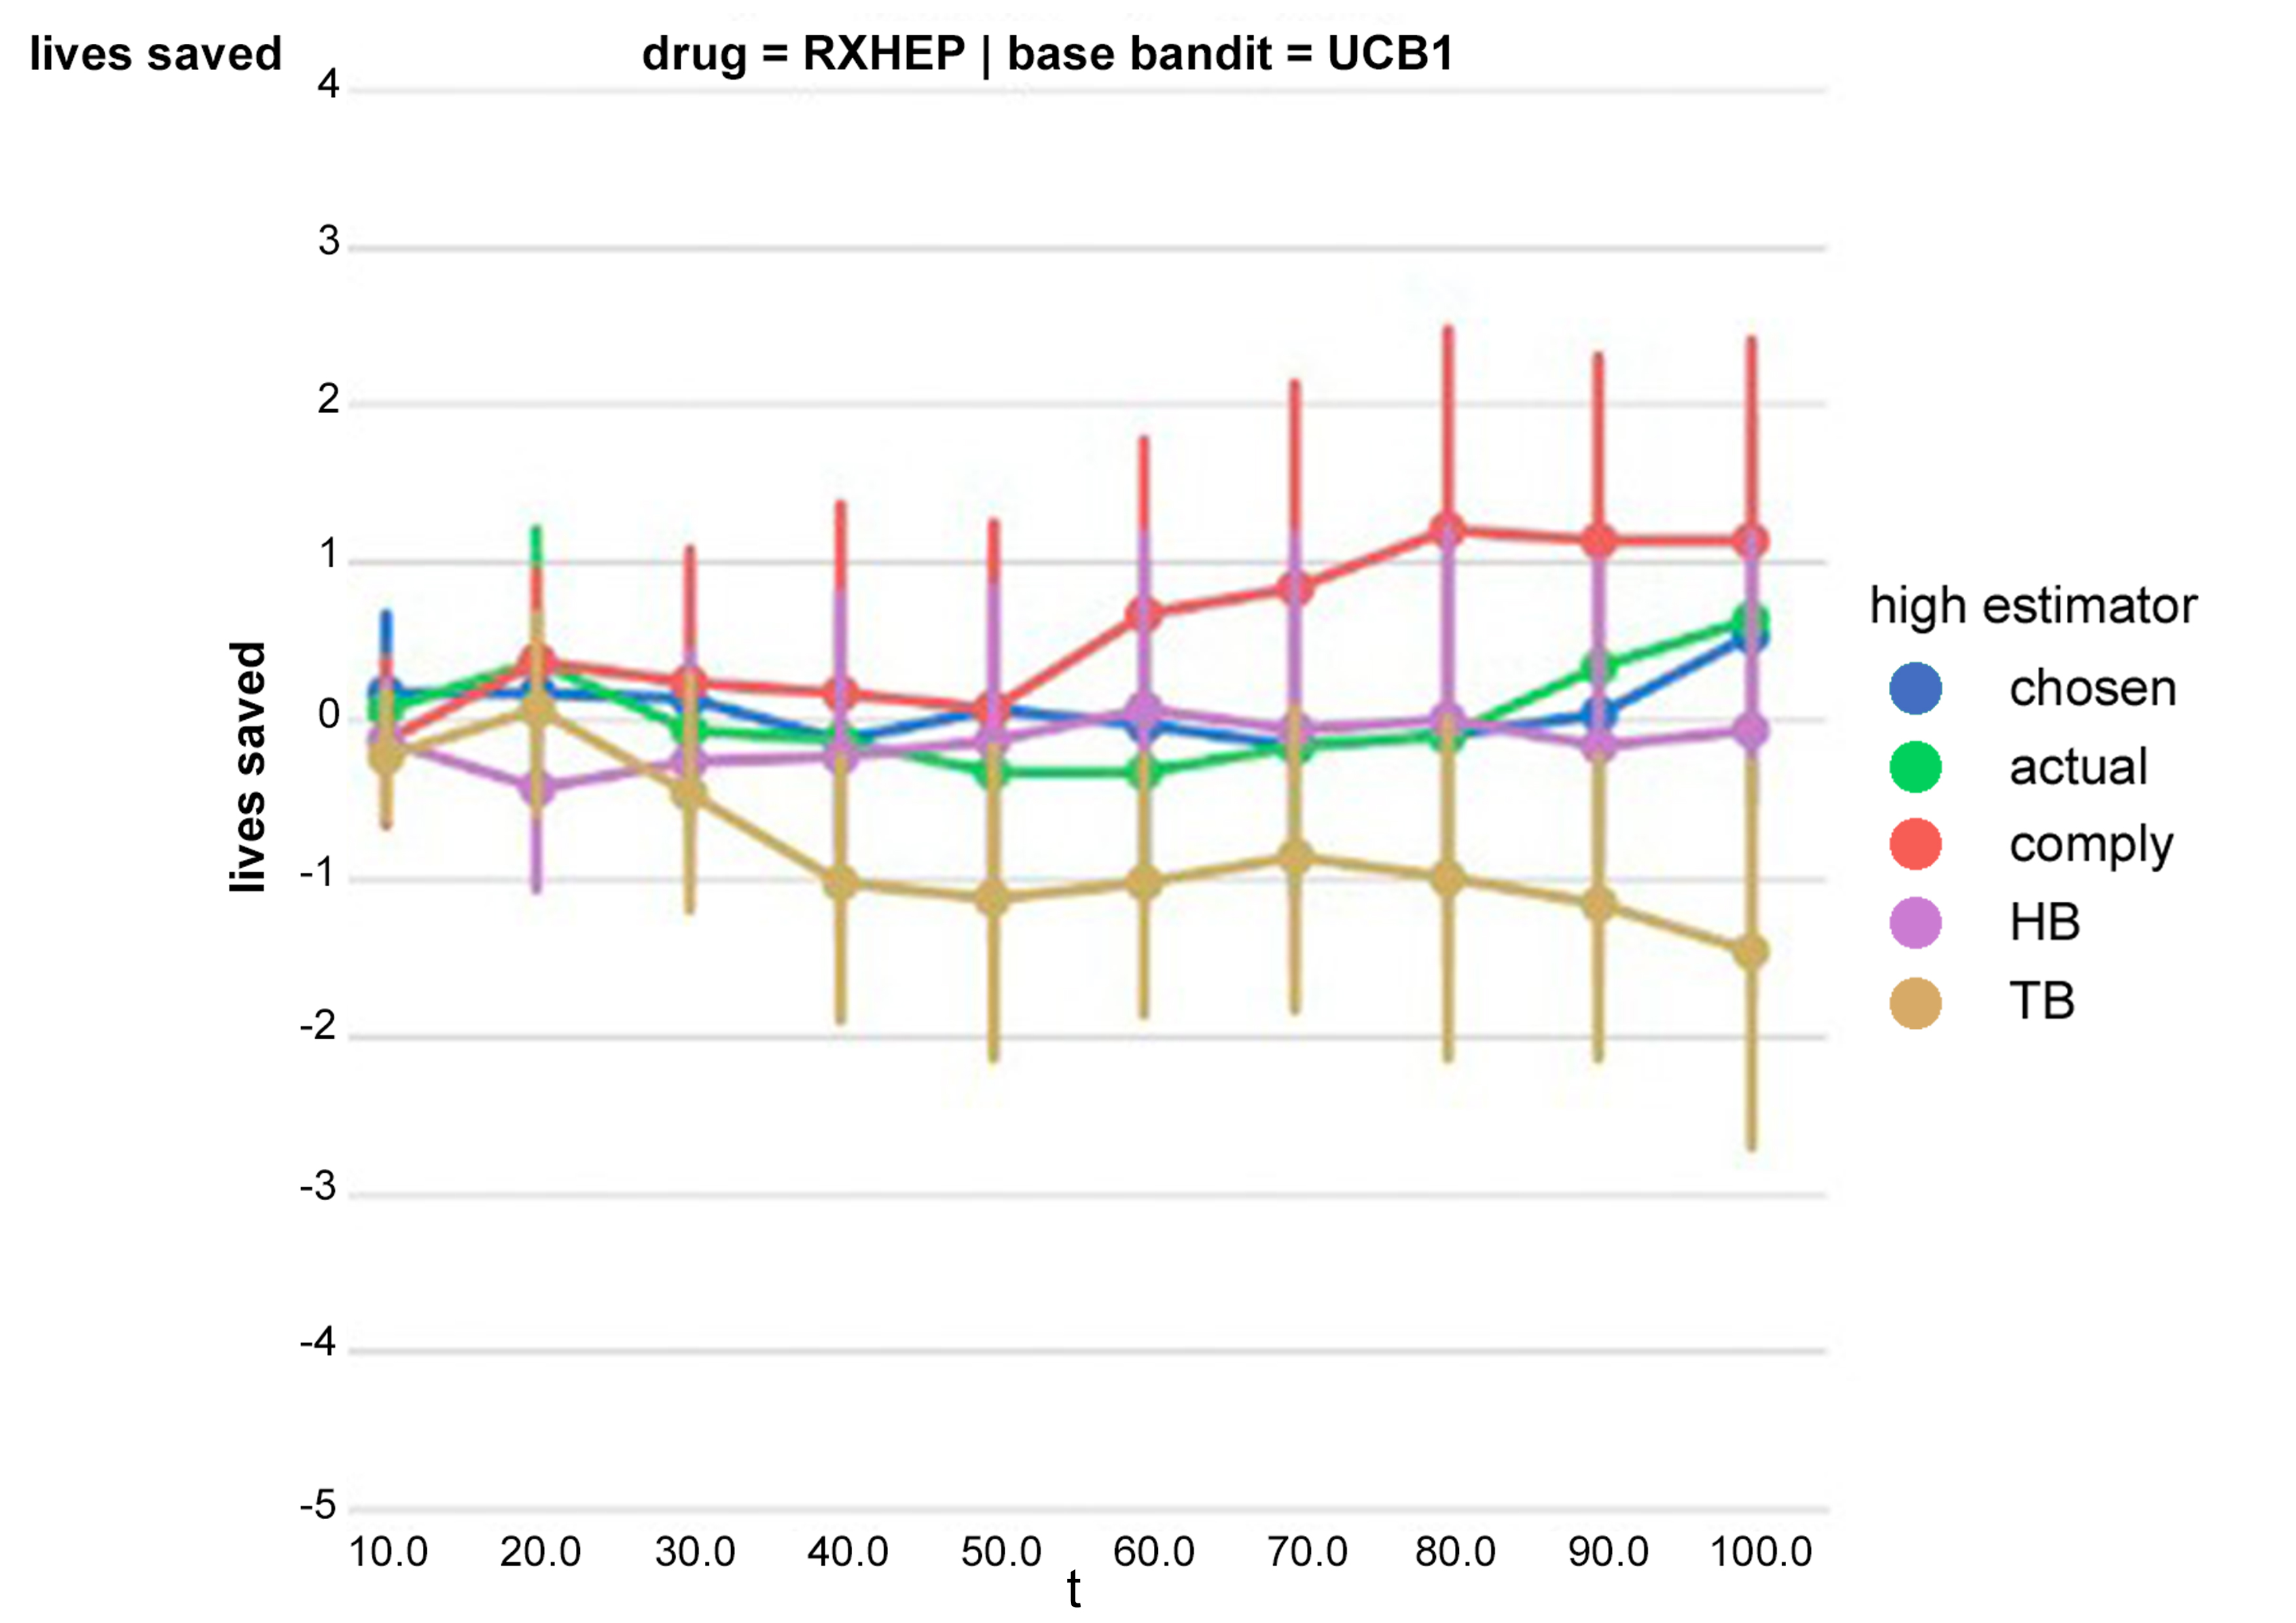
\includegraphics[width=1\columnwidth]{bandit/figs/ex2-3.jpg}\hspace{1cm}
%	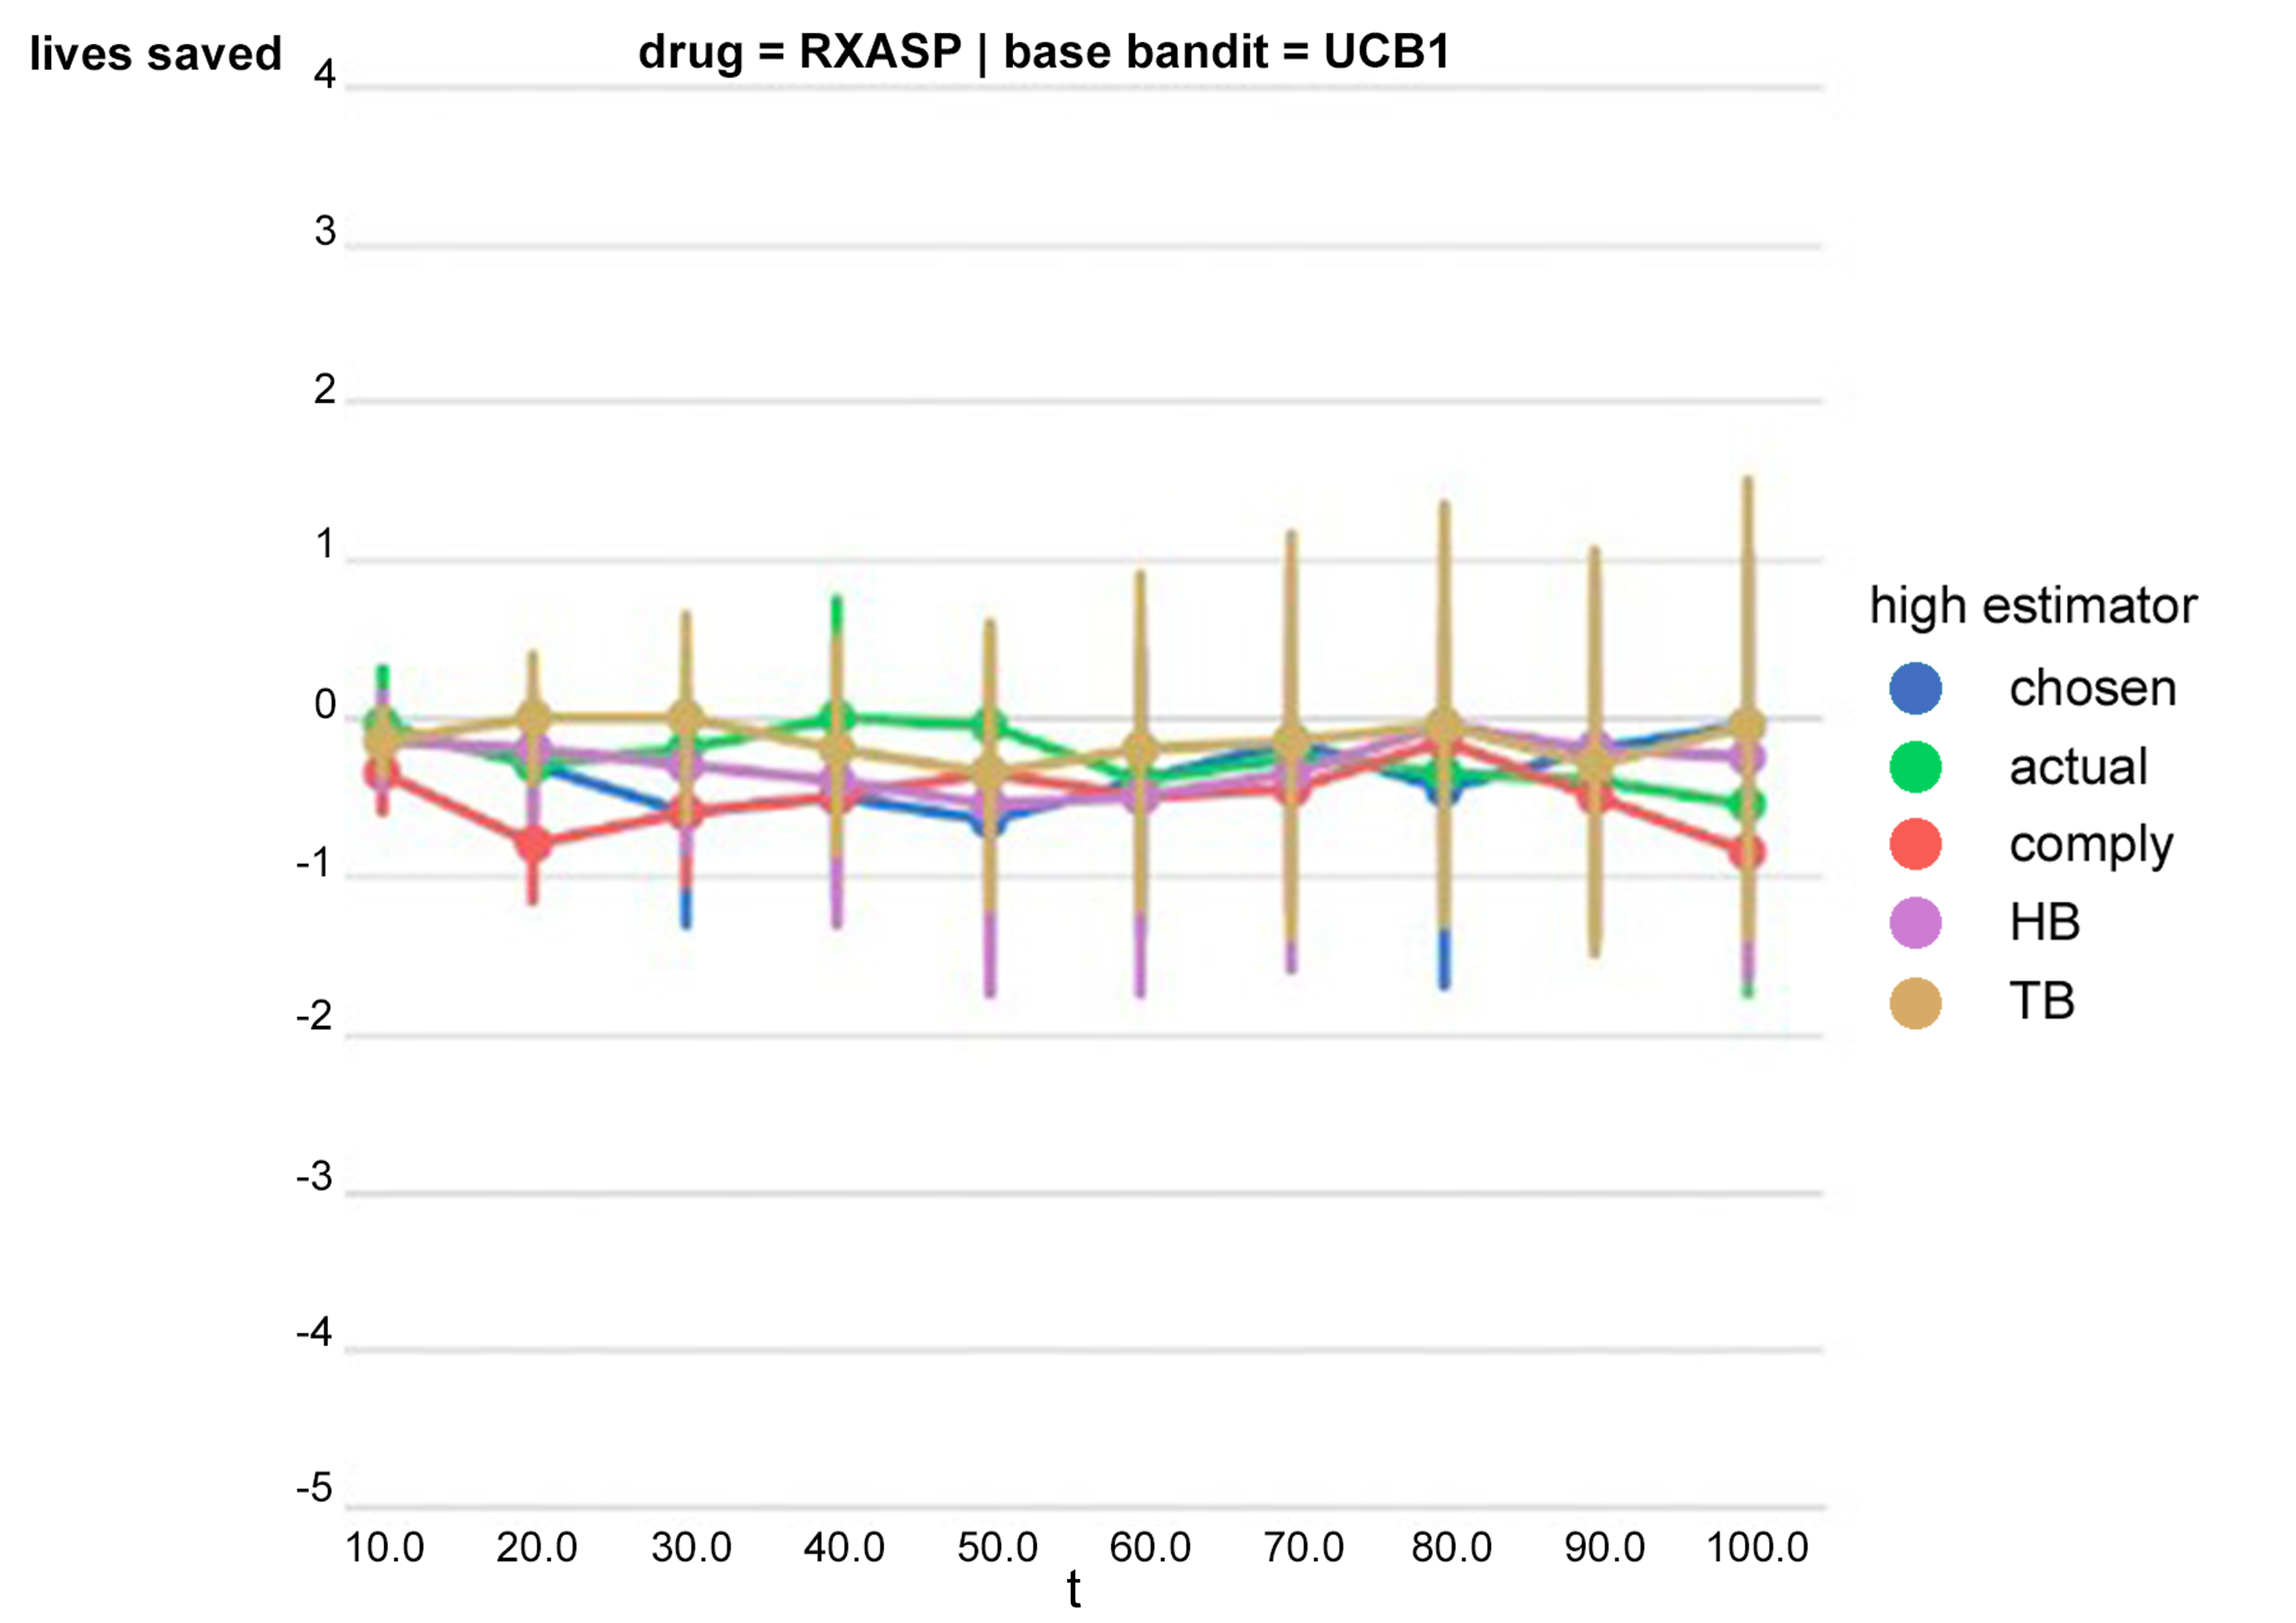
\includegraphics[width=1\columnwidth]{bandit/figs/ex2-4.jpg}\hspace{1cm}
%
%	\caption{Worse than random regret across estimators with naive uses of compliance awareness with simulated data from 100 simulations sampled from a model of a harmful treatment that is profound by selection into treatment.}
%\end{figure}



\subsection{Short time periods}

The second simulation concerns small $T$. A motivation for very small $T$ adaptive clinical trials is provided by rare diseases. The overall size of the patient population is very restricted in this setting.
The priors for the mechanisms of action are also often poorly understood, so potential alternative treatments can have radically different probabilities of success. 
We simulated a $T=12$ adaptive trial, a not uncommon size of clinical trials in rare diseases or neonatal populations. We used binary outcomes, with two treatments and expected rewards drawn uniformly from the unit interval, and compliance drawn uniformly at random. We sampled 1,000 such simulations; results can be seen in Fig.~\eqref{fig:ex3}.
While our bounds are vacuous in this setting, it is interesting that there is, on average, an improvement when taking the noncompliance information into account.


\begin{figure}[t]
	\centering	
	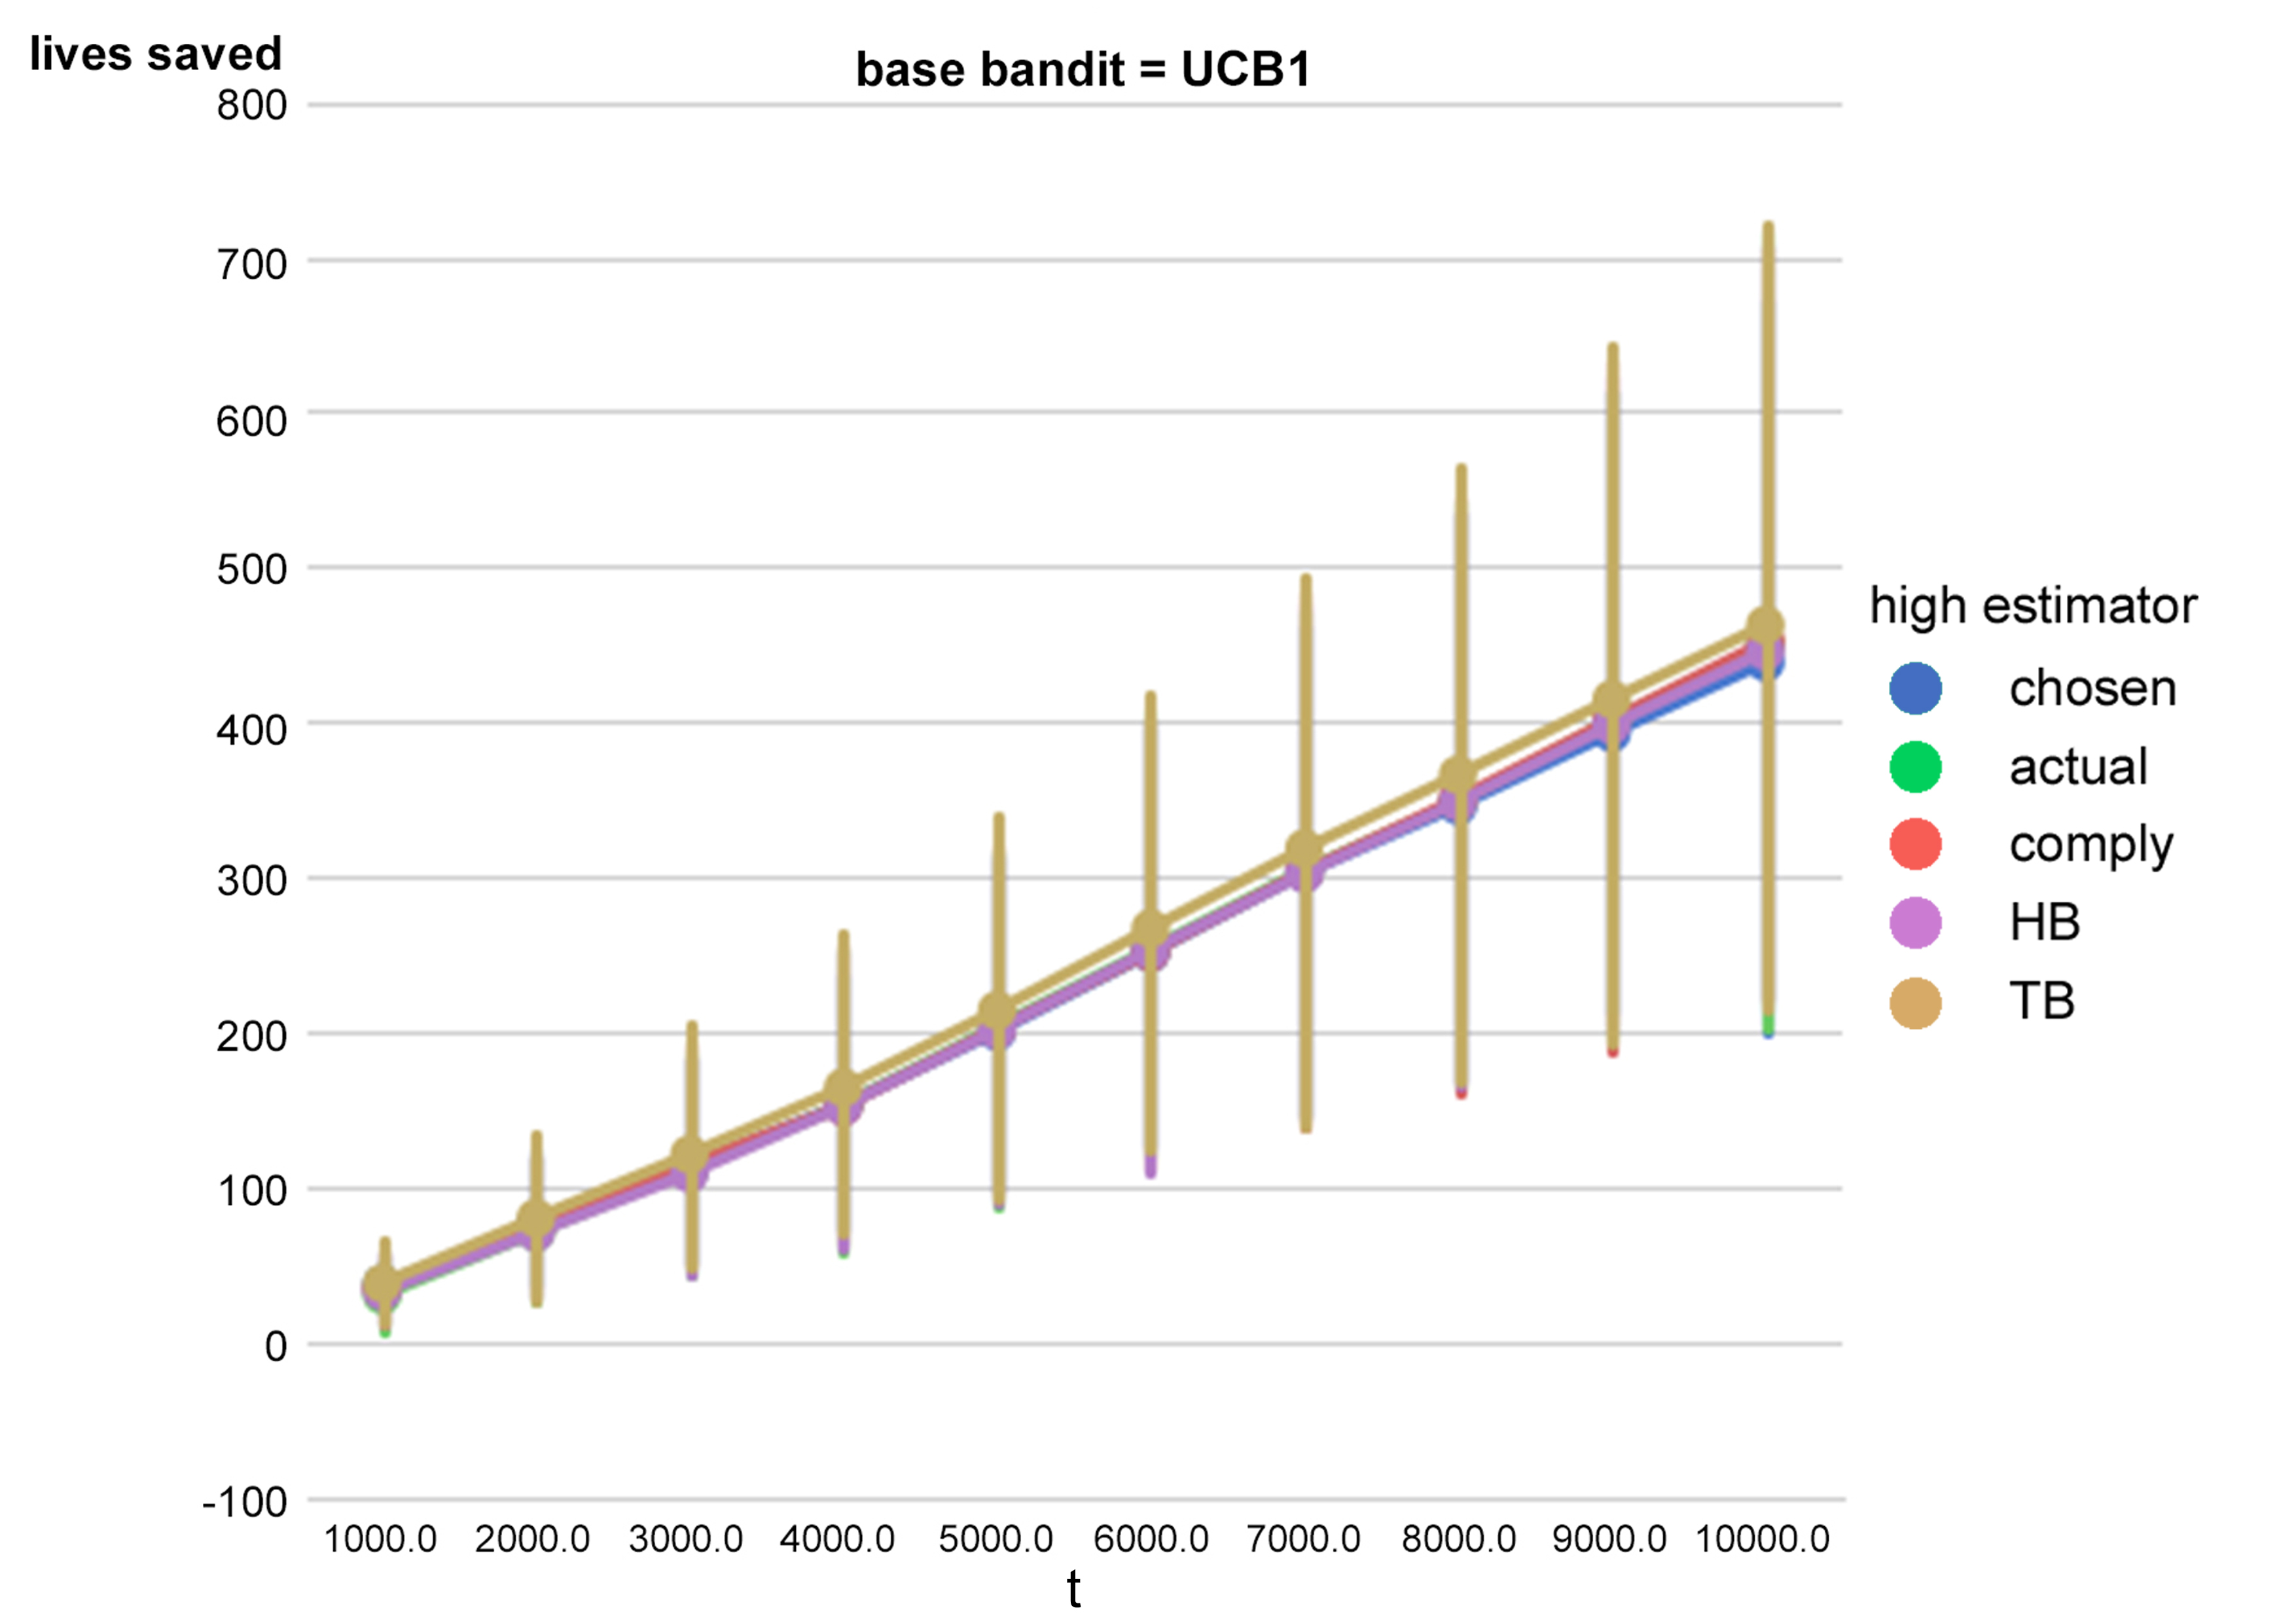
\includegraphics[width=0.9\textwidth]{bandit/figs/ex3-1.jpg}\hspace{1cm}
	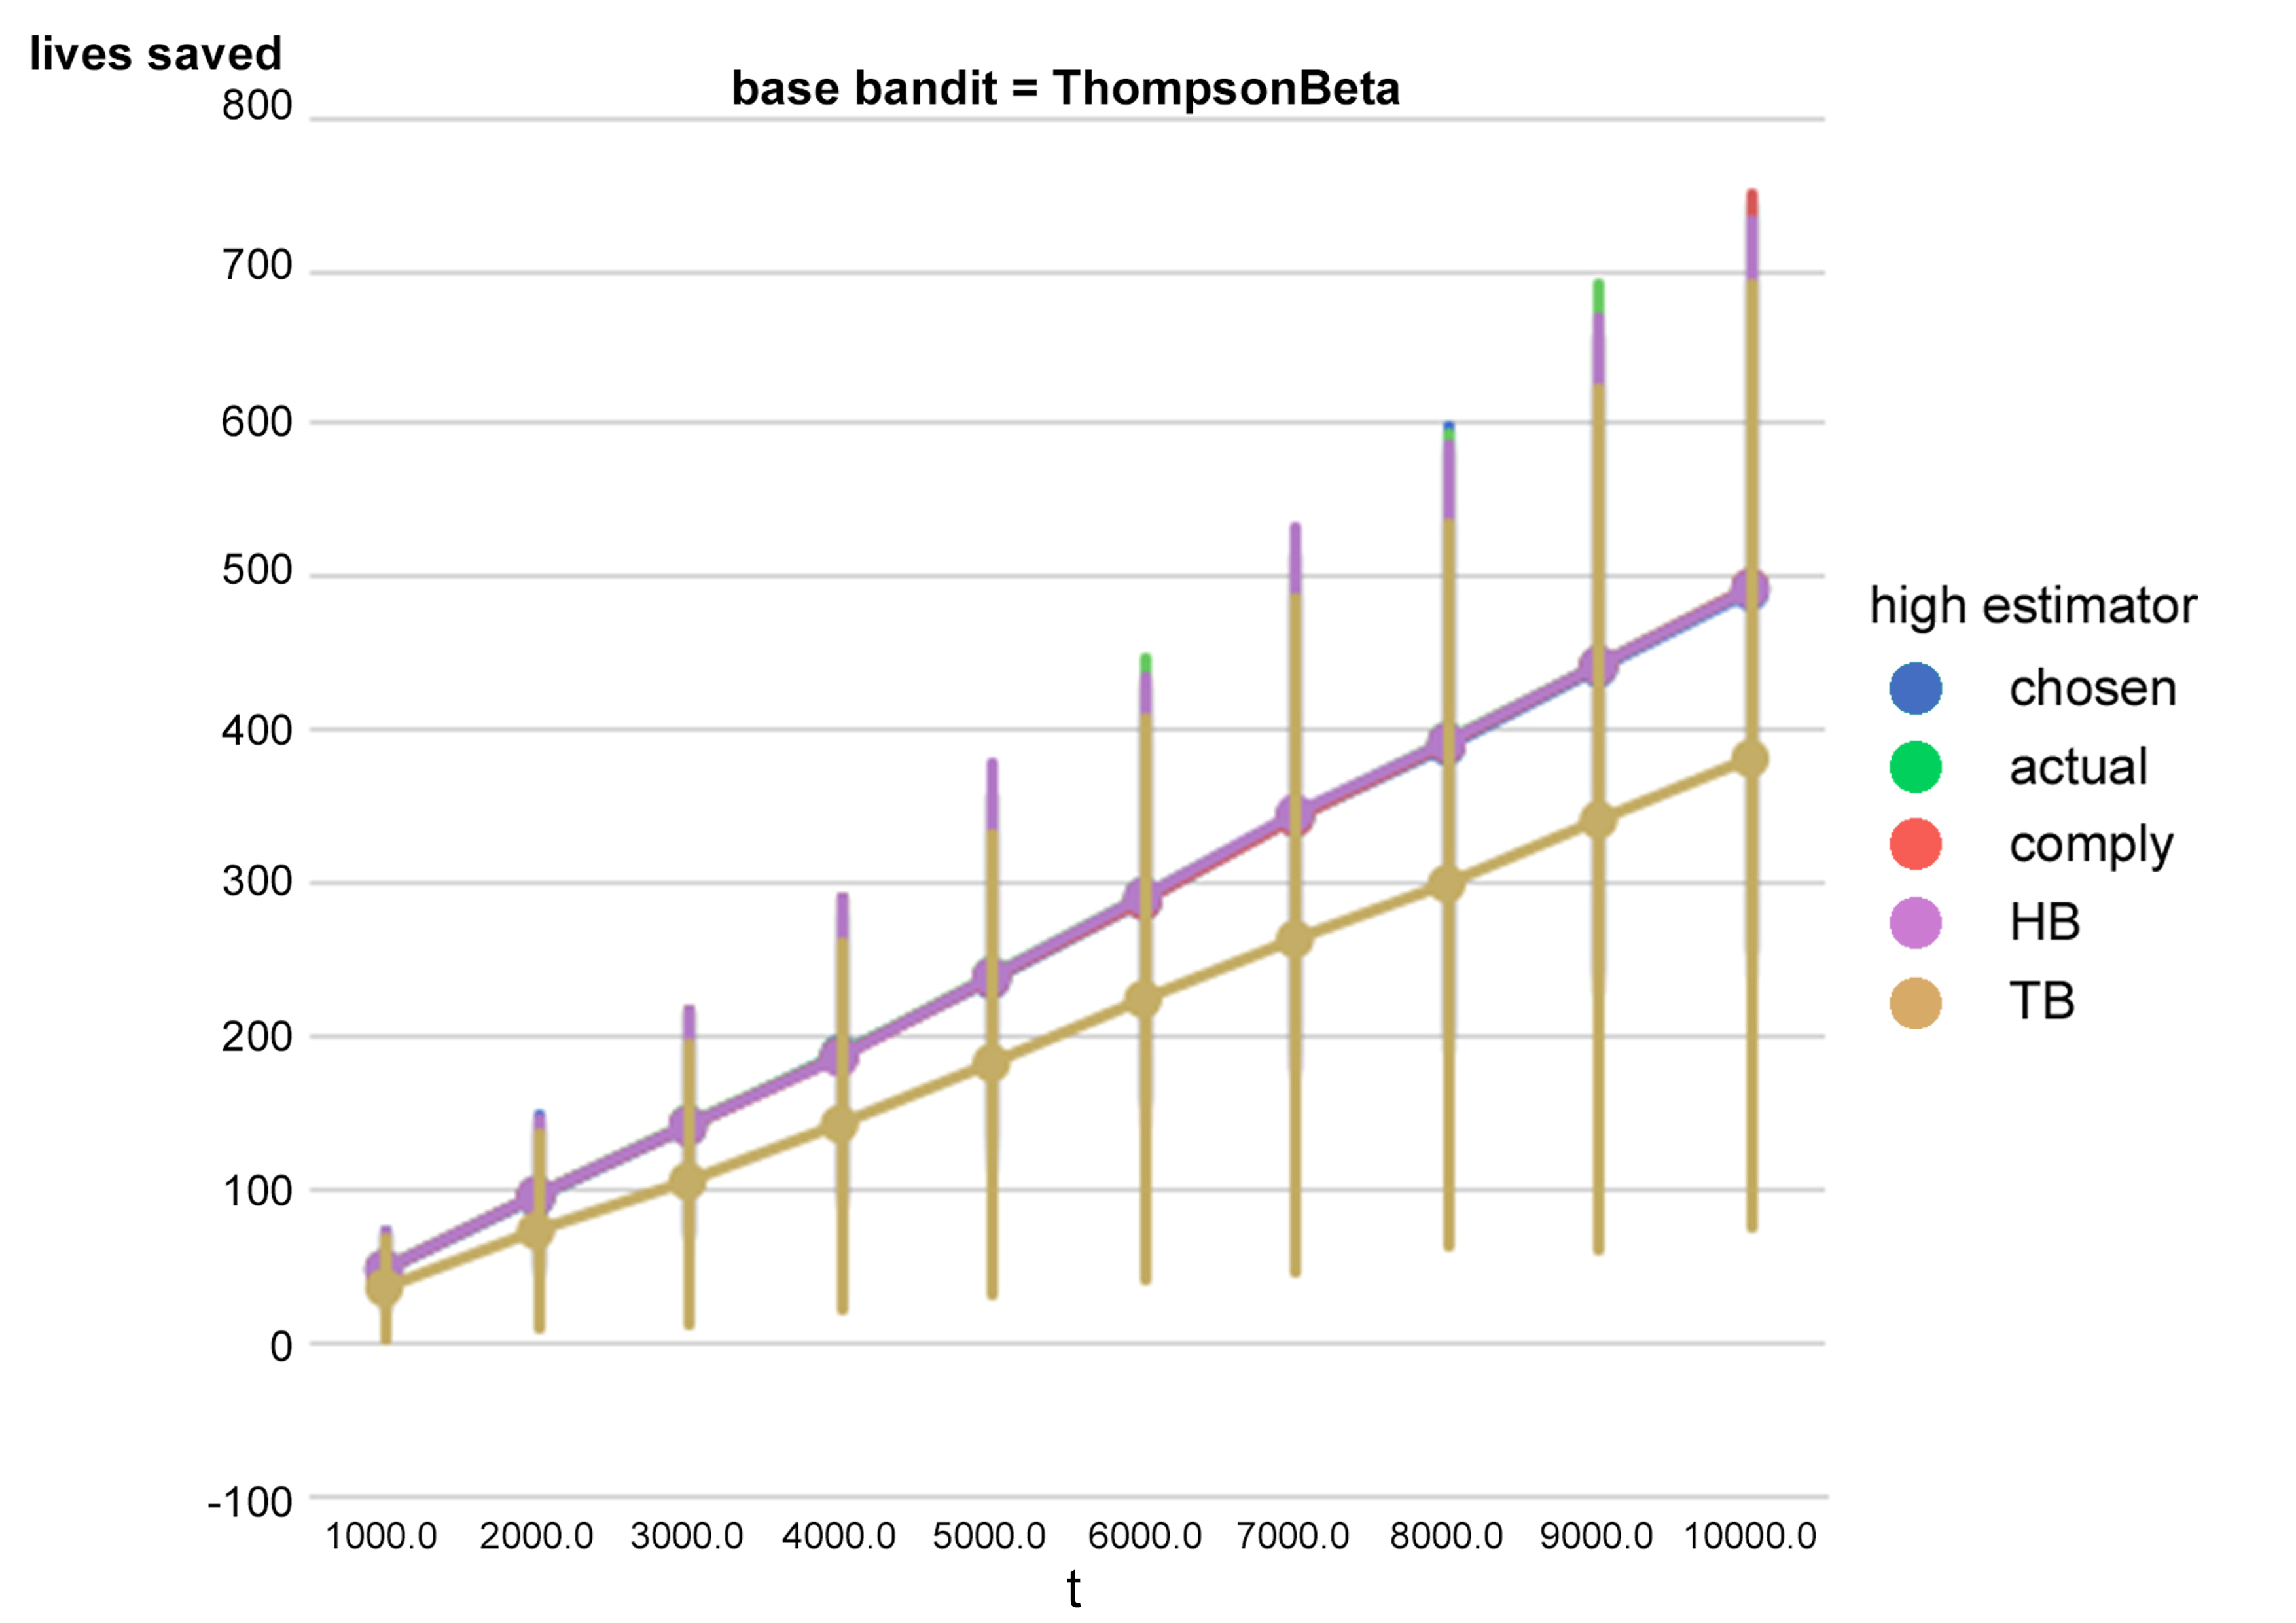
\includegraphics[width=0.9\textwidth]{bandit/figs/ex3-2.jpg}\hspace{1cm}
	\caption{Results from 1000 simulations with $T=12$ and synthetic data:with two treatments and expected rewards drawn uniformly from the unit interval, and compliance uniformly at random.}	
	\end{figure}
\begin{figure}[t]

	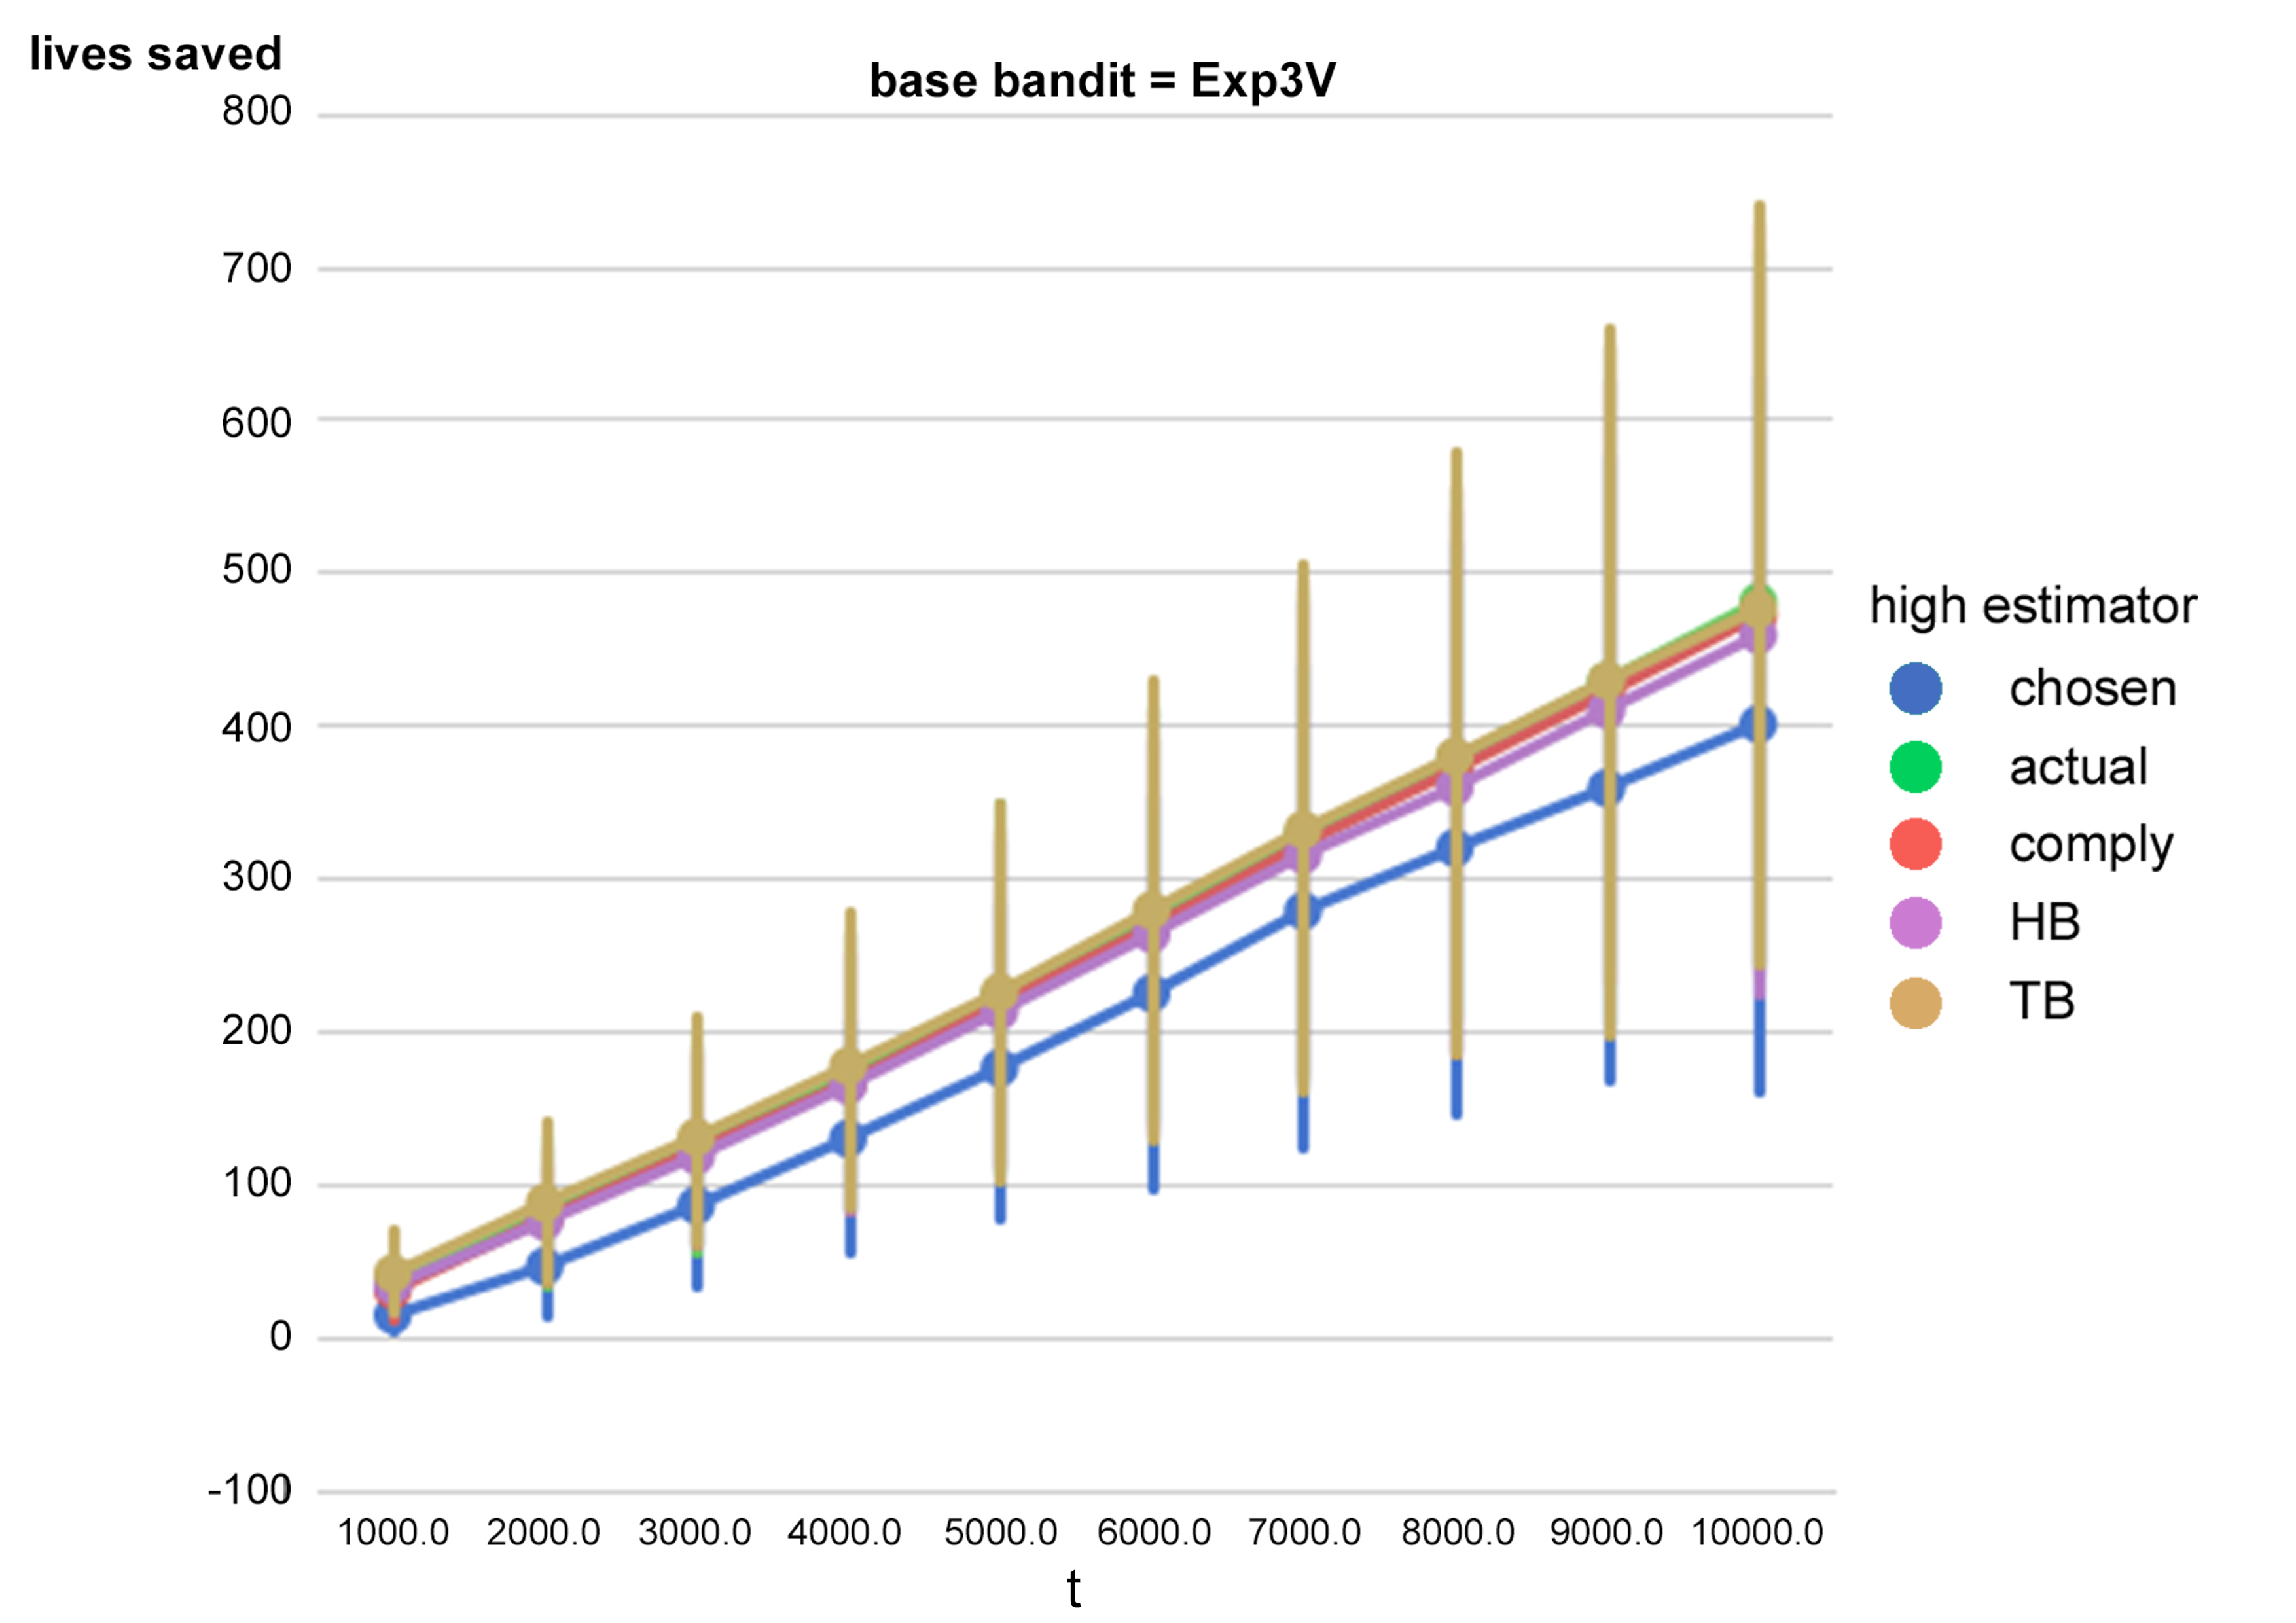
\includegraphics[width=0.9\textwidth]{bandit/figs/ex3-3.jpg}\hspace{1cm}
	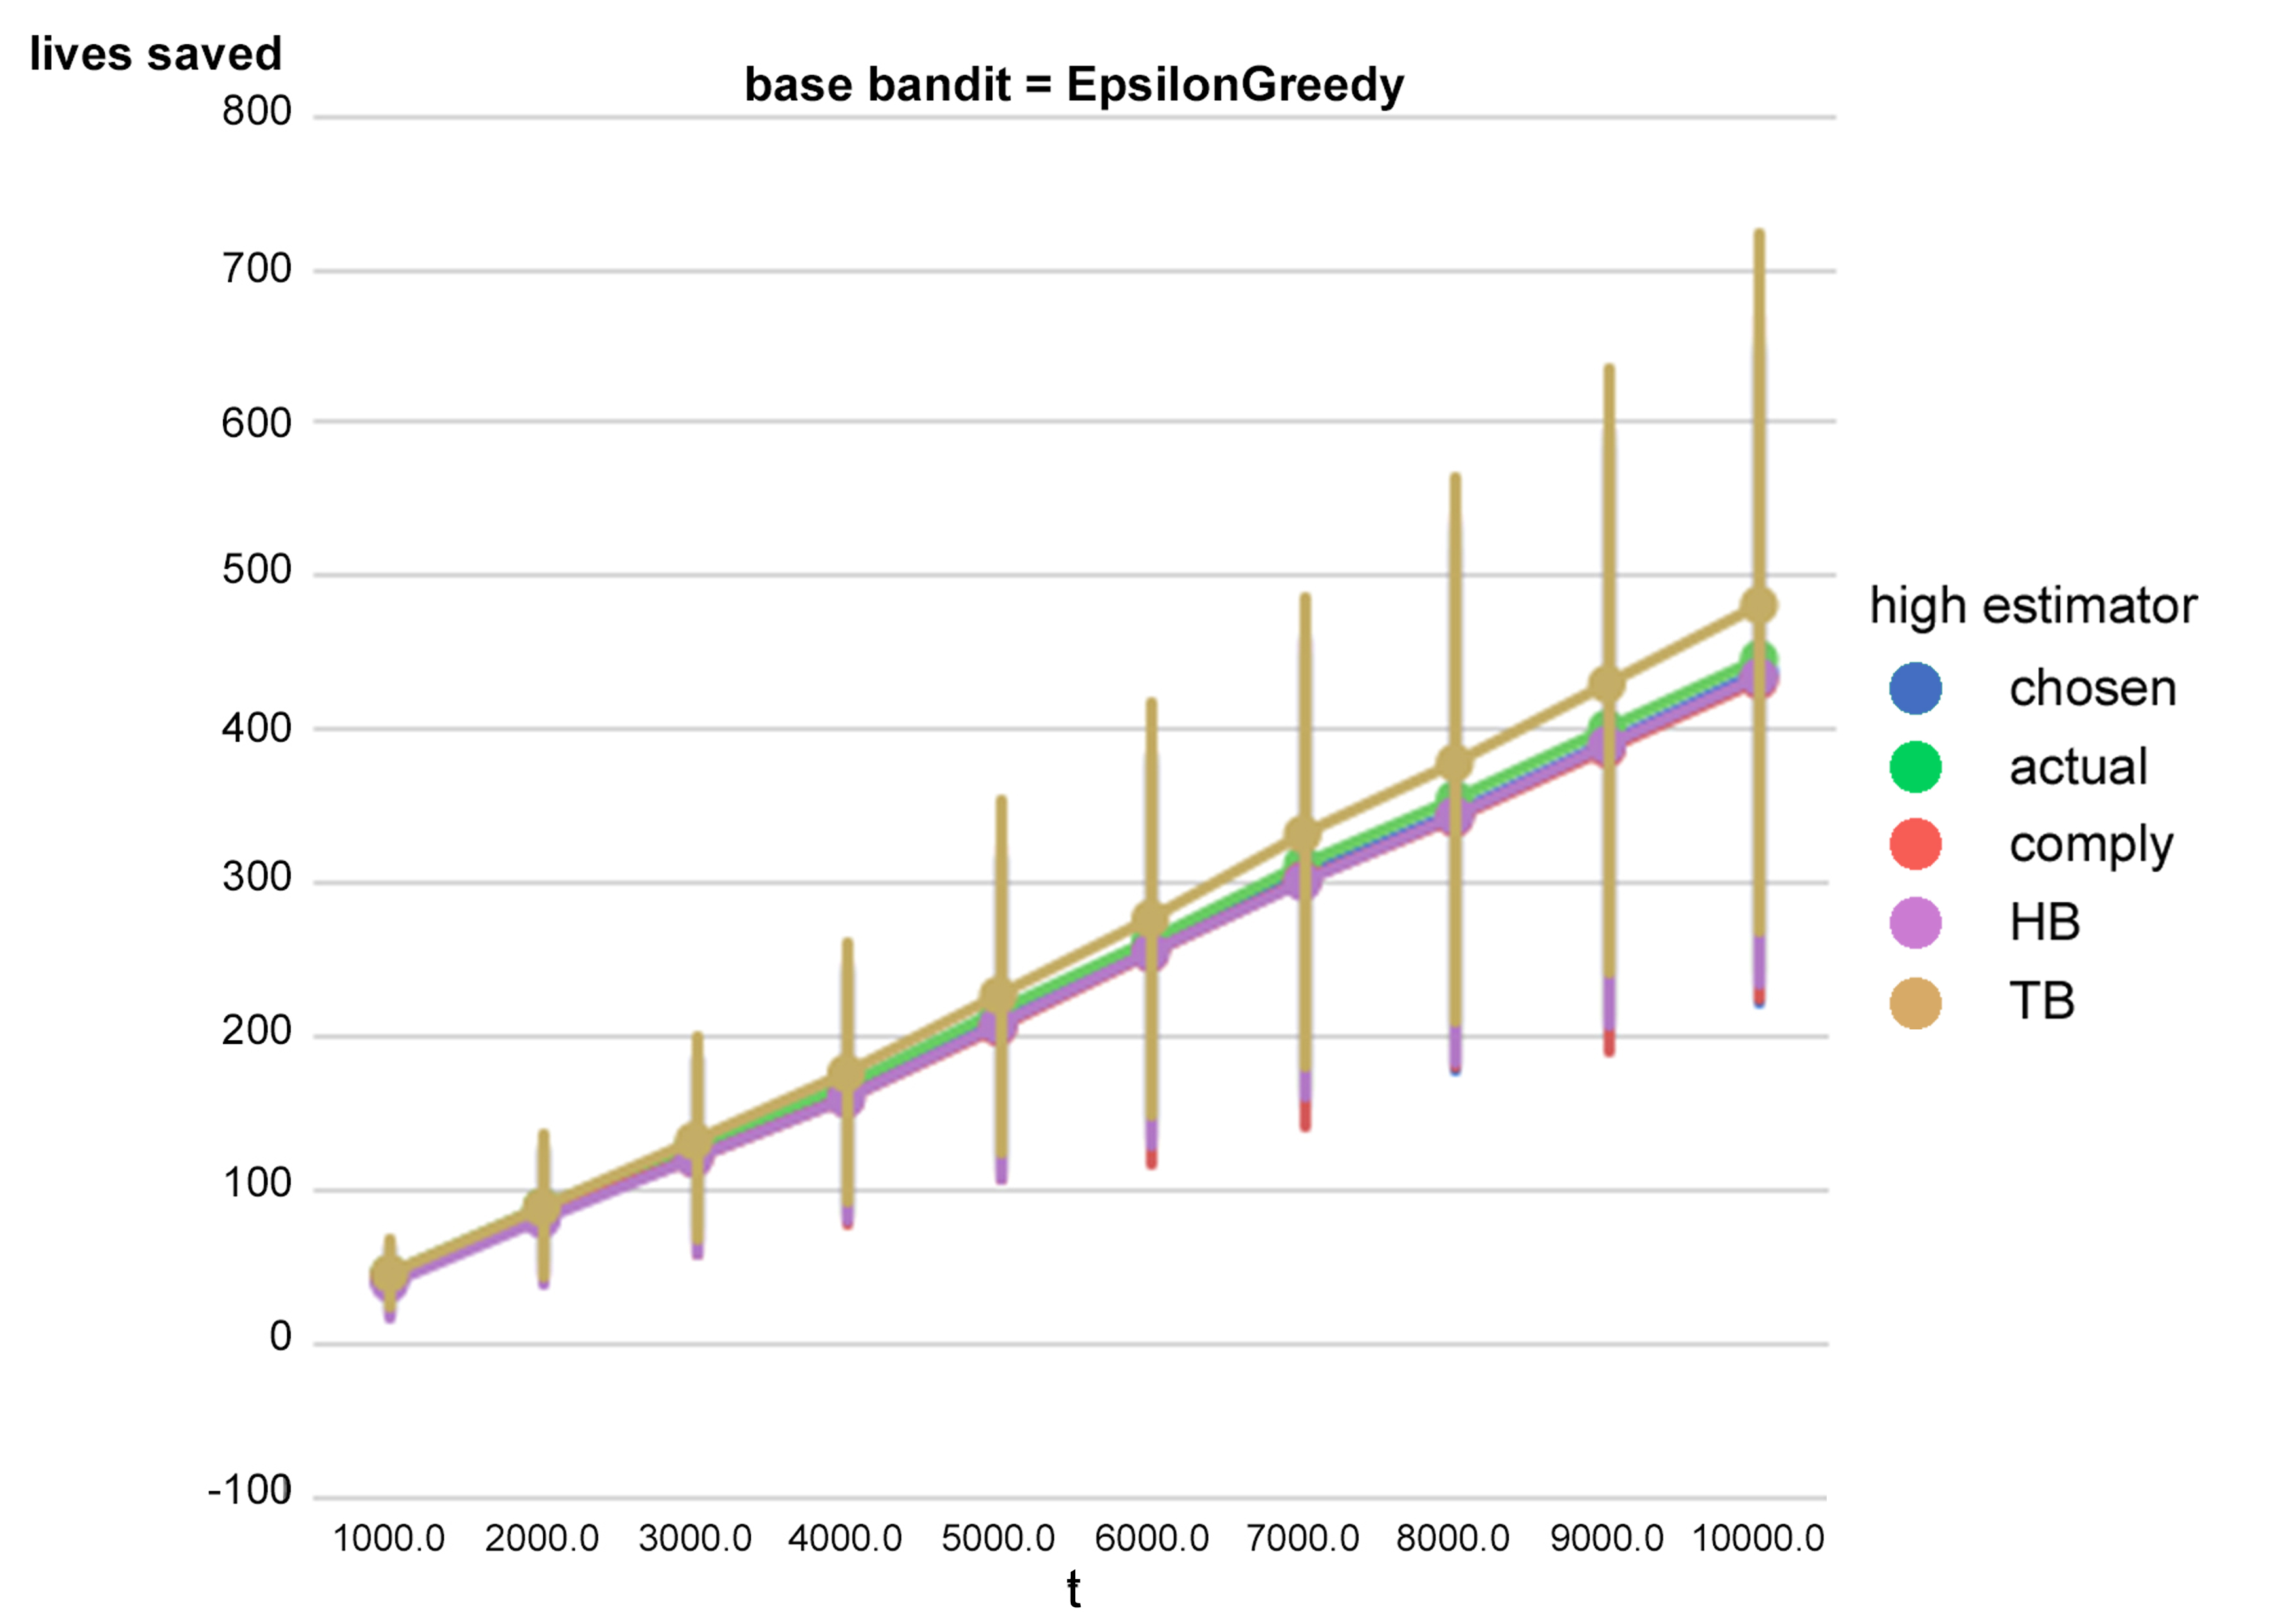
\includegraphics[width=0.9\textwidth]{bandit/figs/ex3-4.jpg}\hspace{1cm}
	
	\label{fig:ex3}
	\caption{Results from 1000 simulations with $T=12$ and synthetic data:with two treatments and expected rewards drawn uniformly from the unit interval, and compliance uniformly at random.}
\end{figure}





\subsection{Noncompliance for Best Arm}


A natural scenario for noncompliance, and one that offers substantial potential, is when the subject is better informed than the algorithm and realizes they know a better alternative. 
This provides potentially huge practical advantages, especially in situations with very large numbers of a priori low expectation but high variance actions. 
They allow later subjects to benefit from the information that previous subjects bring to the mechanism, while current compliance unaware algorithms not only waste this information but hurt later subjects by unnecessarily raising the apparent variance of the rewards in the arms (since the chosen arm may indeed be very bad relative to the actual arm).
%TODO but what exactly did you do for this simulation???



\begin{figure}[t]
	\centering	
	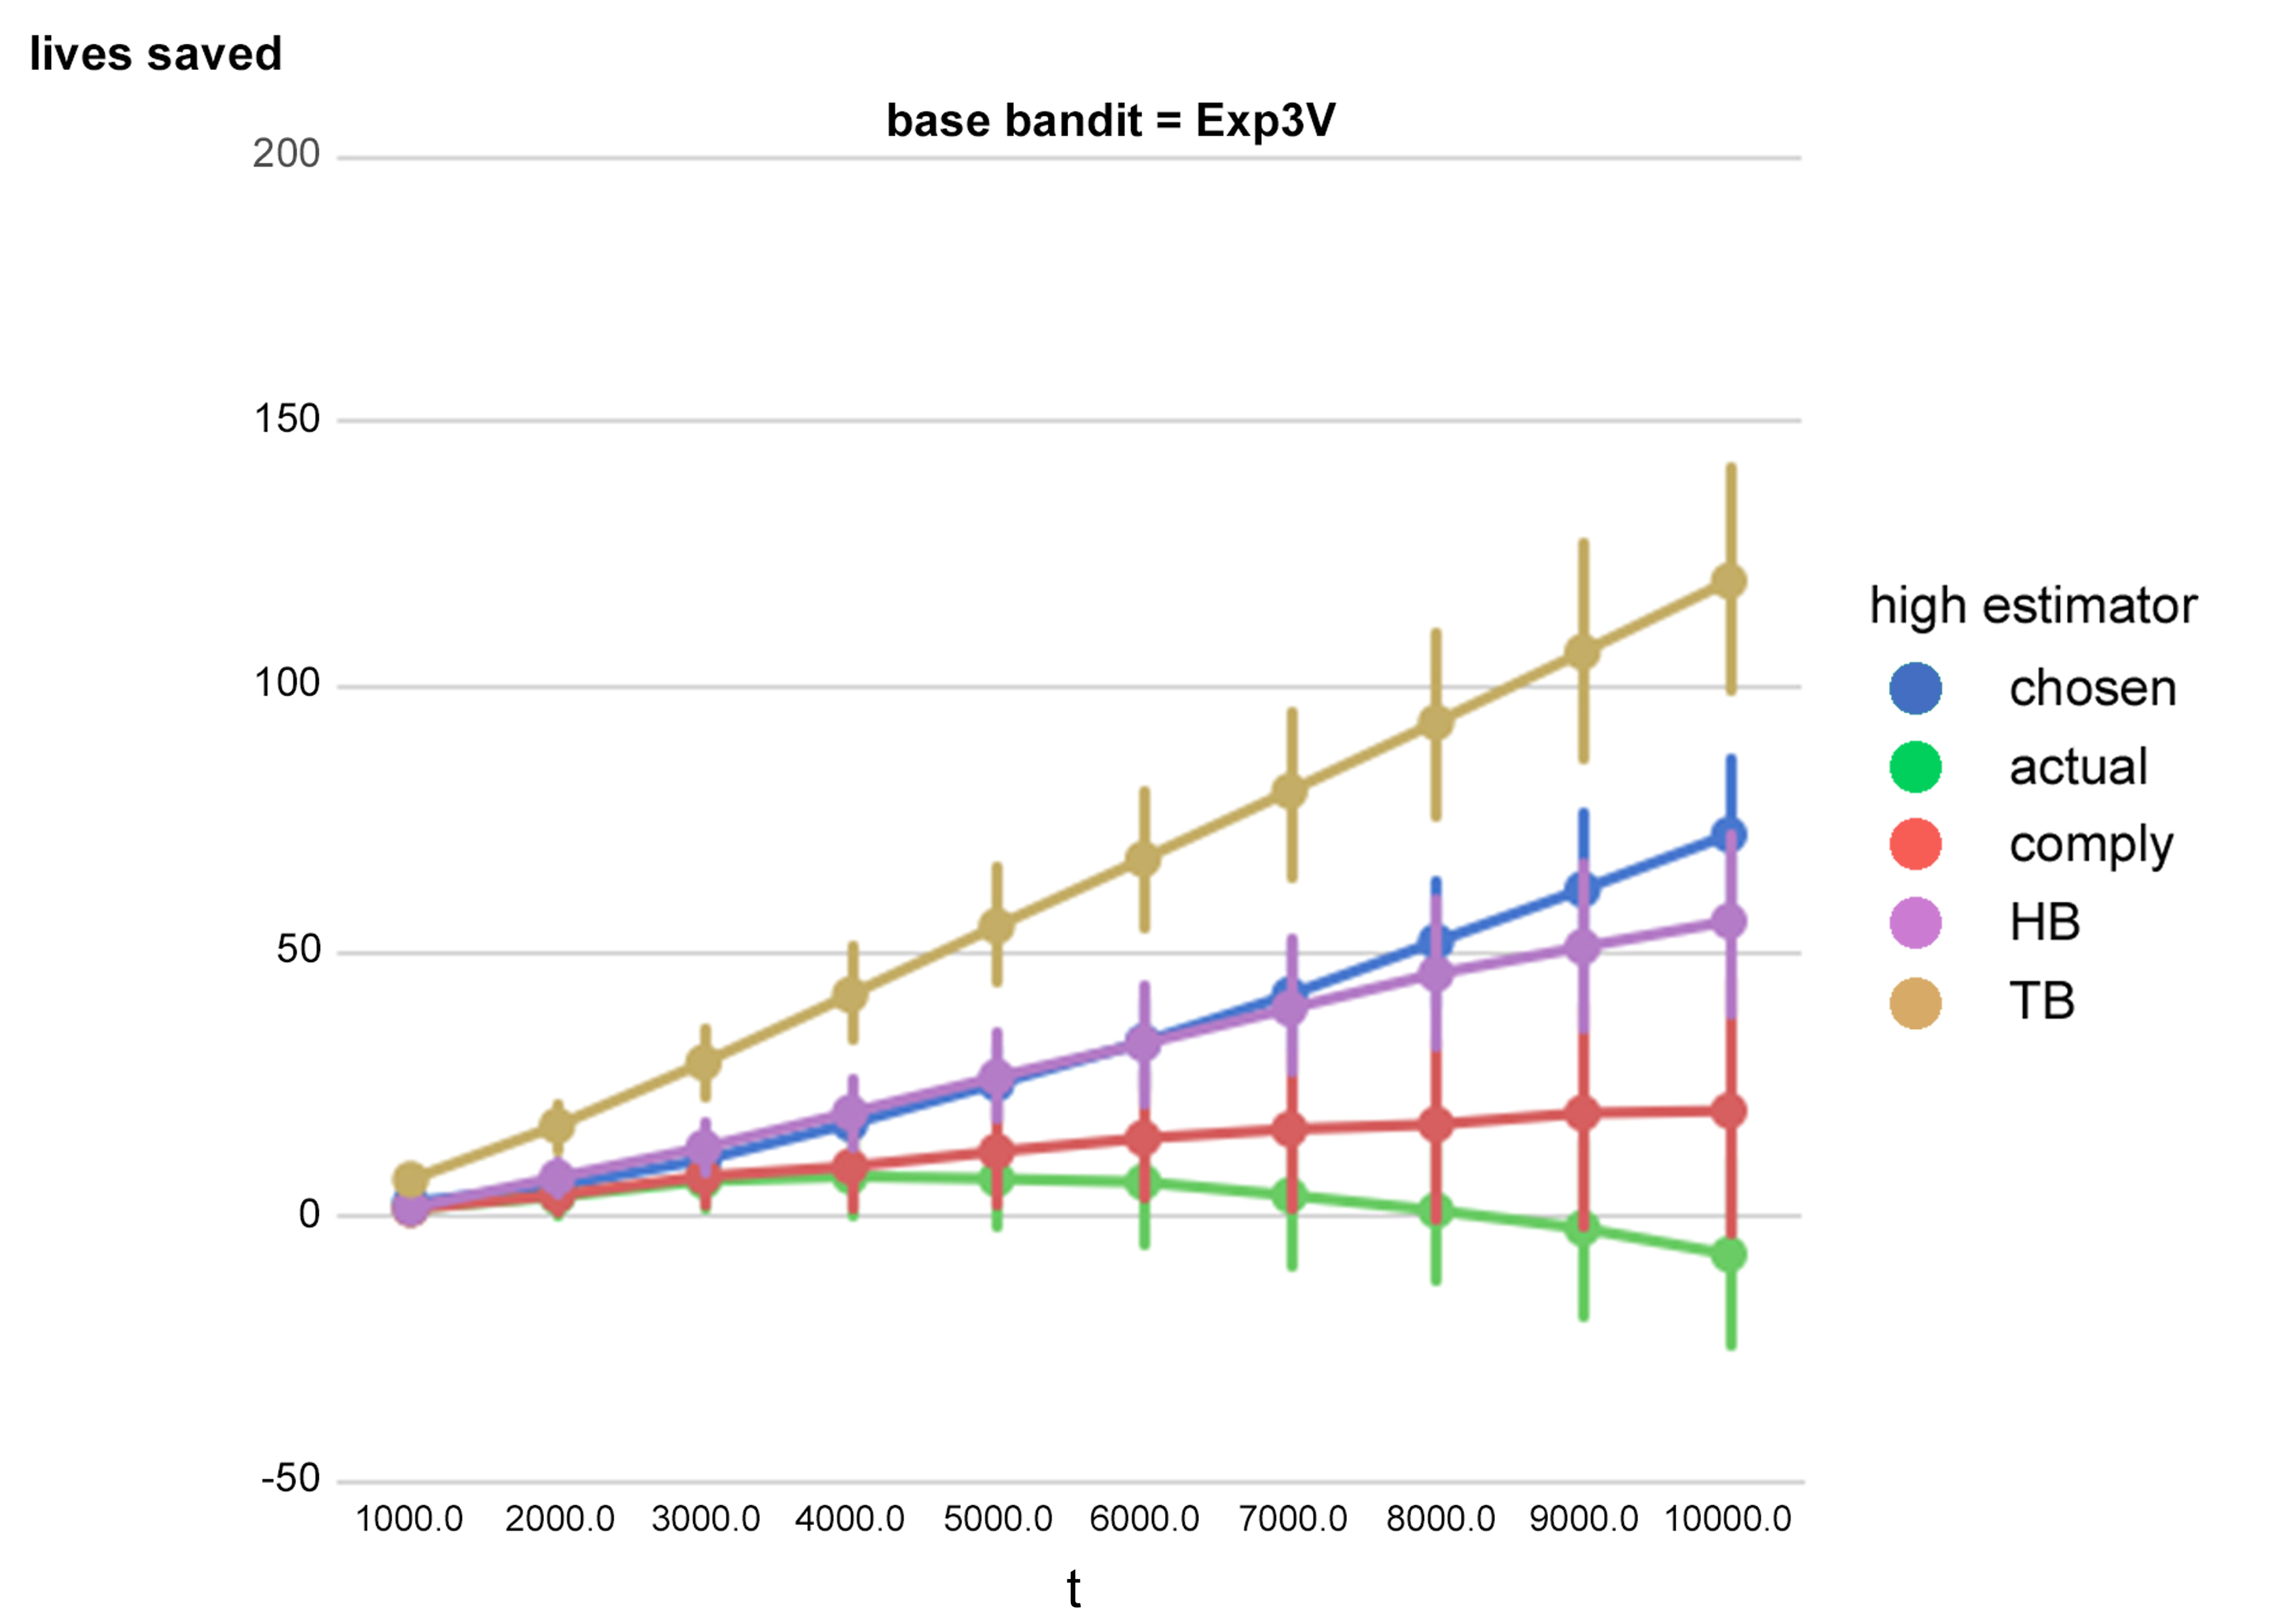
\includegraphics[width=0.9\textwidth]{bandit/figs/ex4-1.jpg}\hspace{1cm}	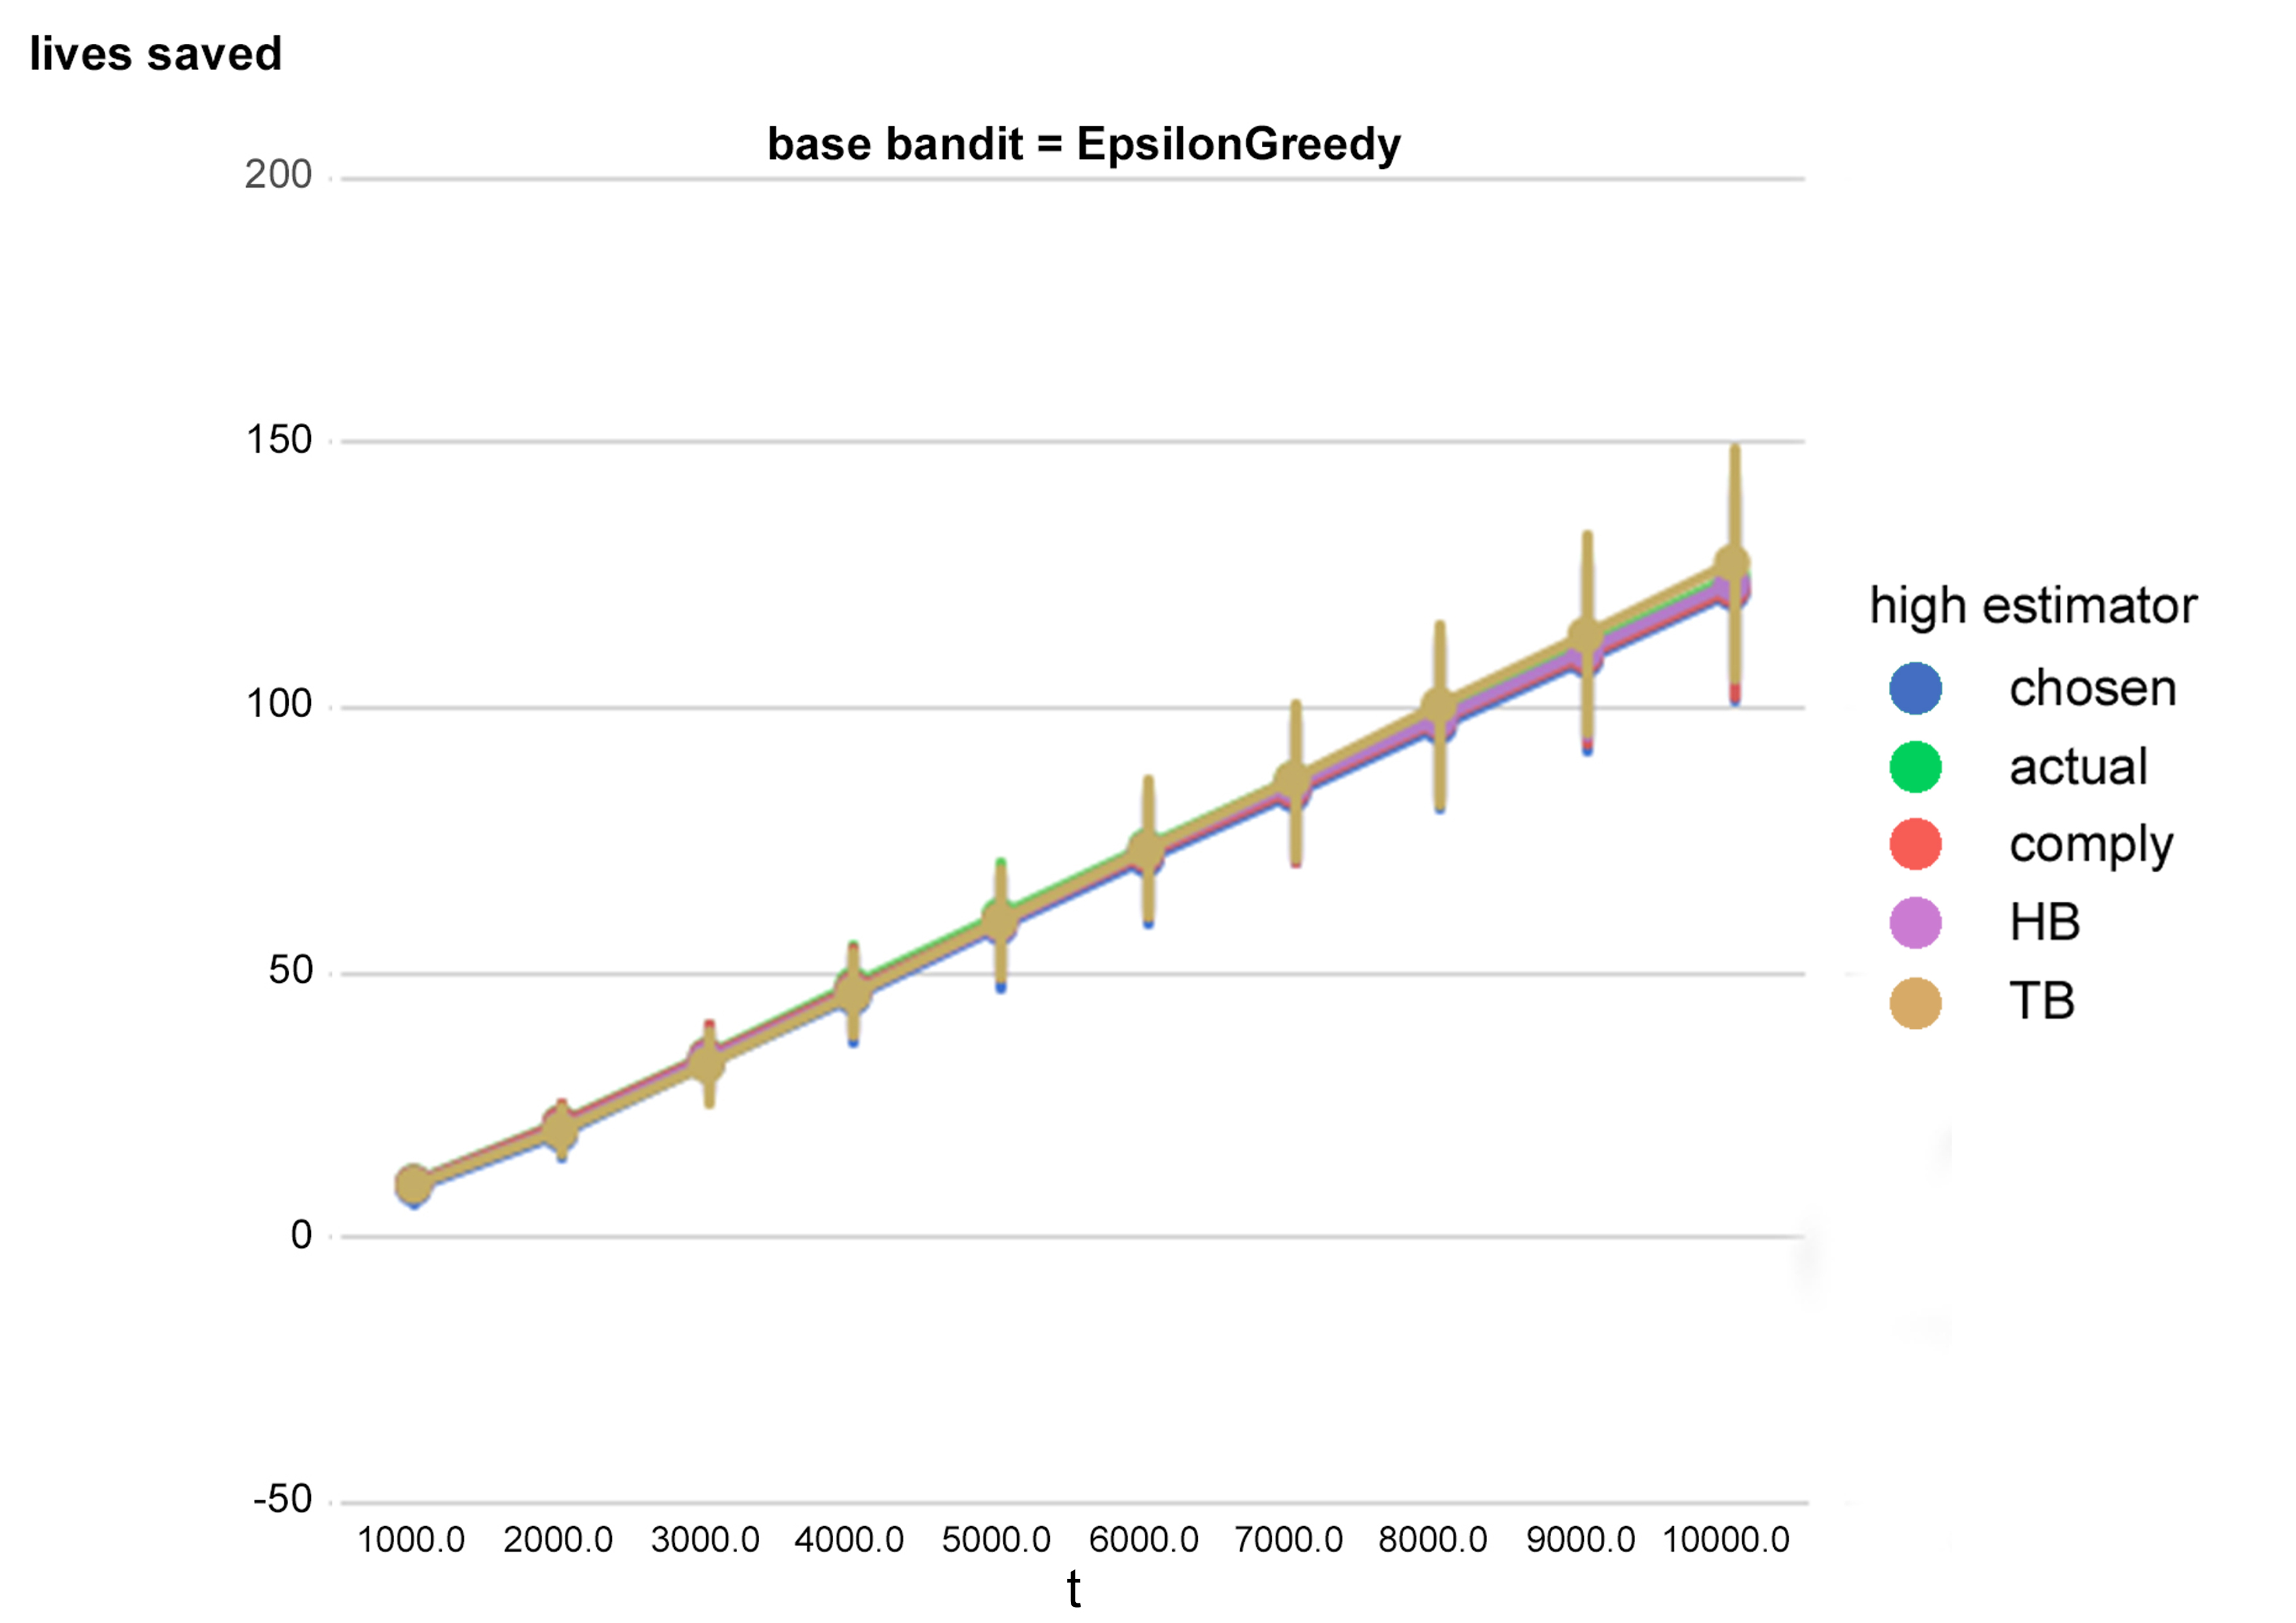
\includegraphics[width=0.9\textwidth]{bandit/figs/ex4-2.jpg}\hspace{1cm}
	\caption{Noncompliance for best arm: 100 simulations from synthetic data of $T=10,000$ with noncompliance proportional to how much better the best arm is than the algorithm selection.}
\end{figure}	
\begin{figure}[t]
	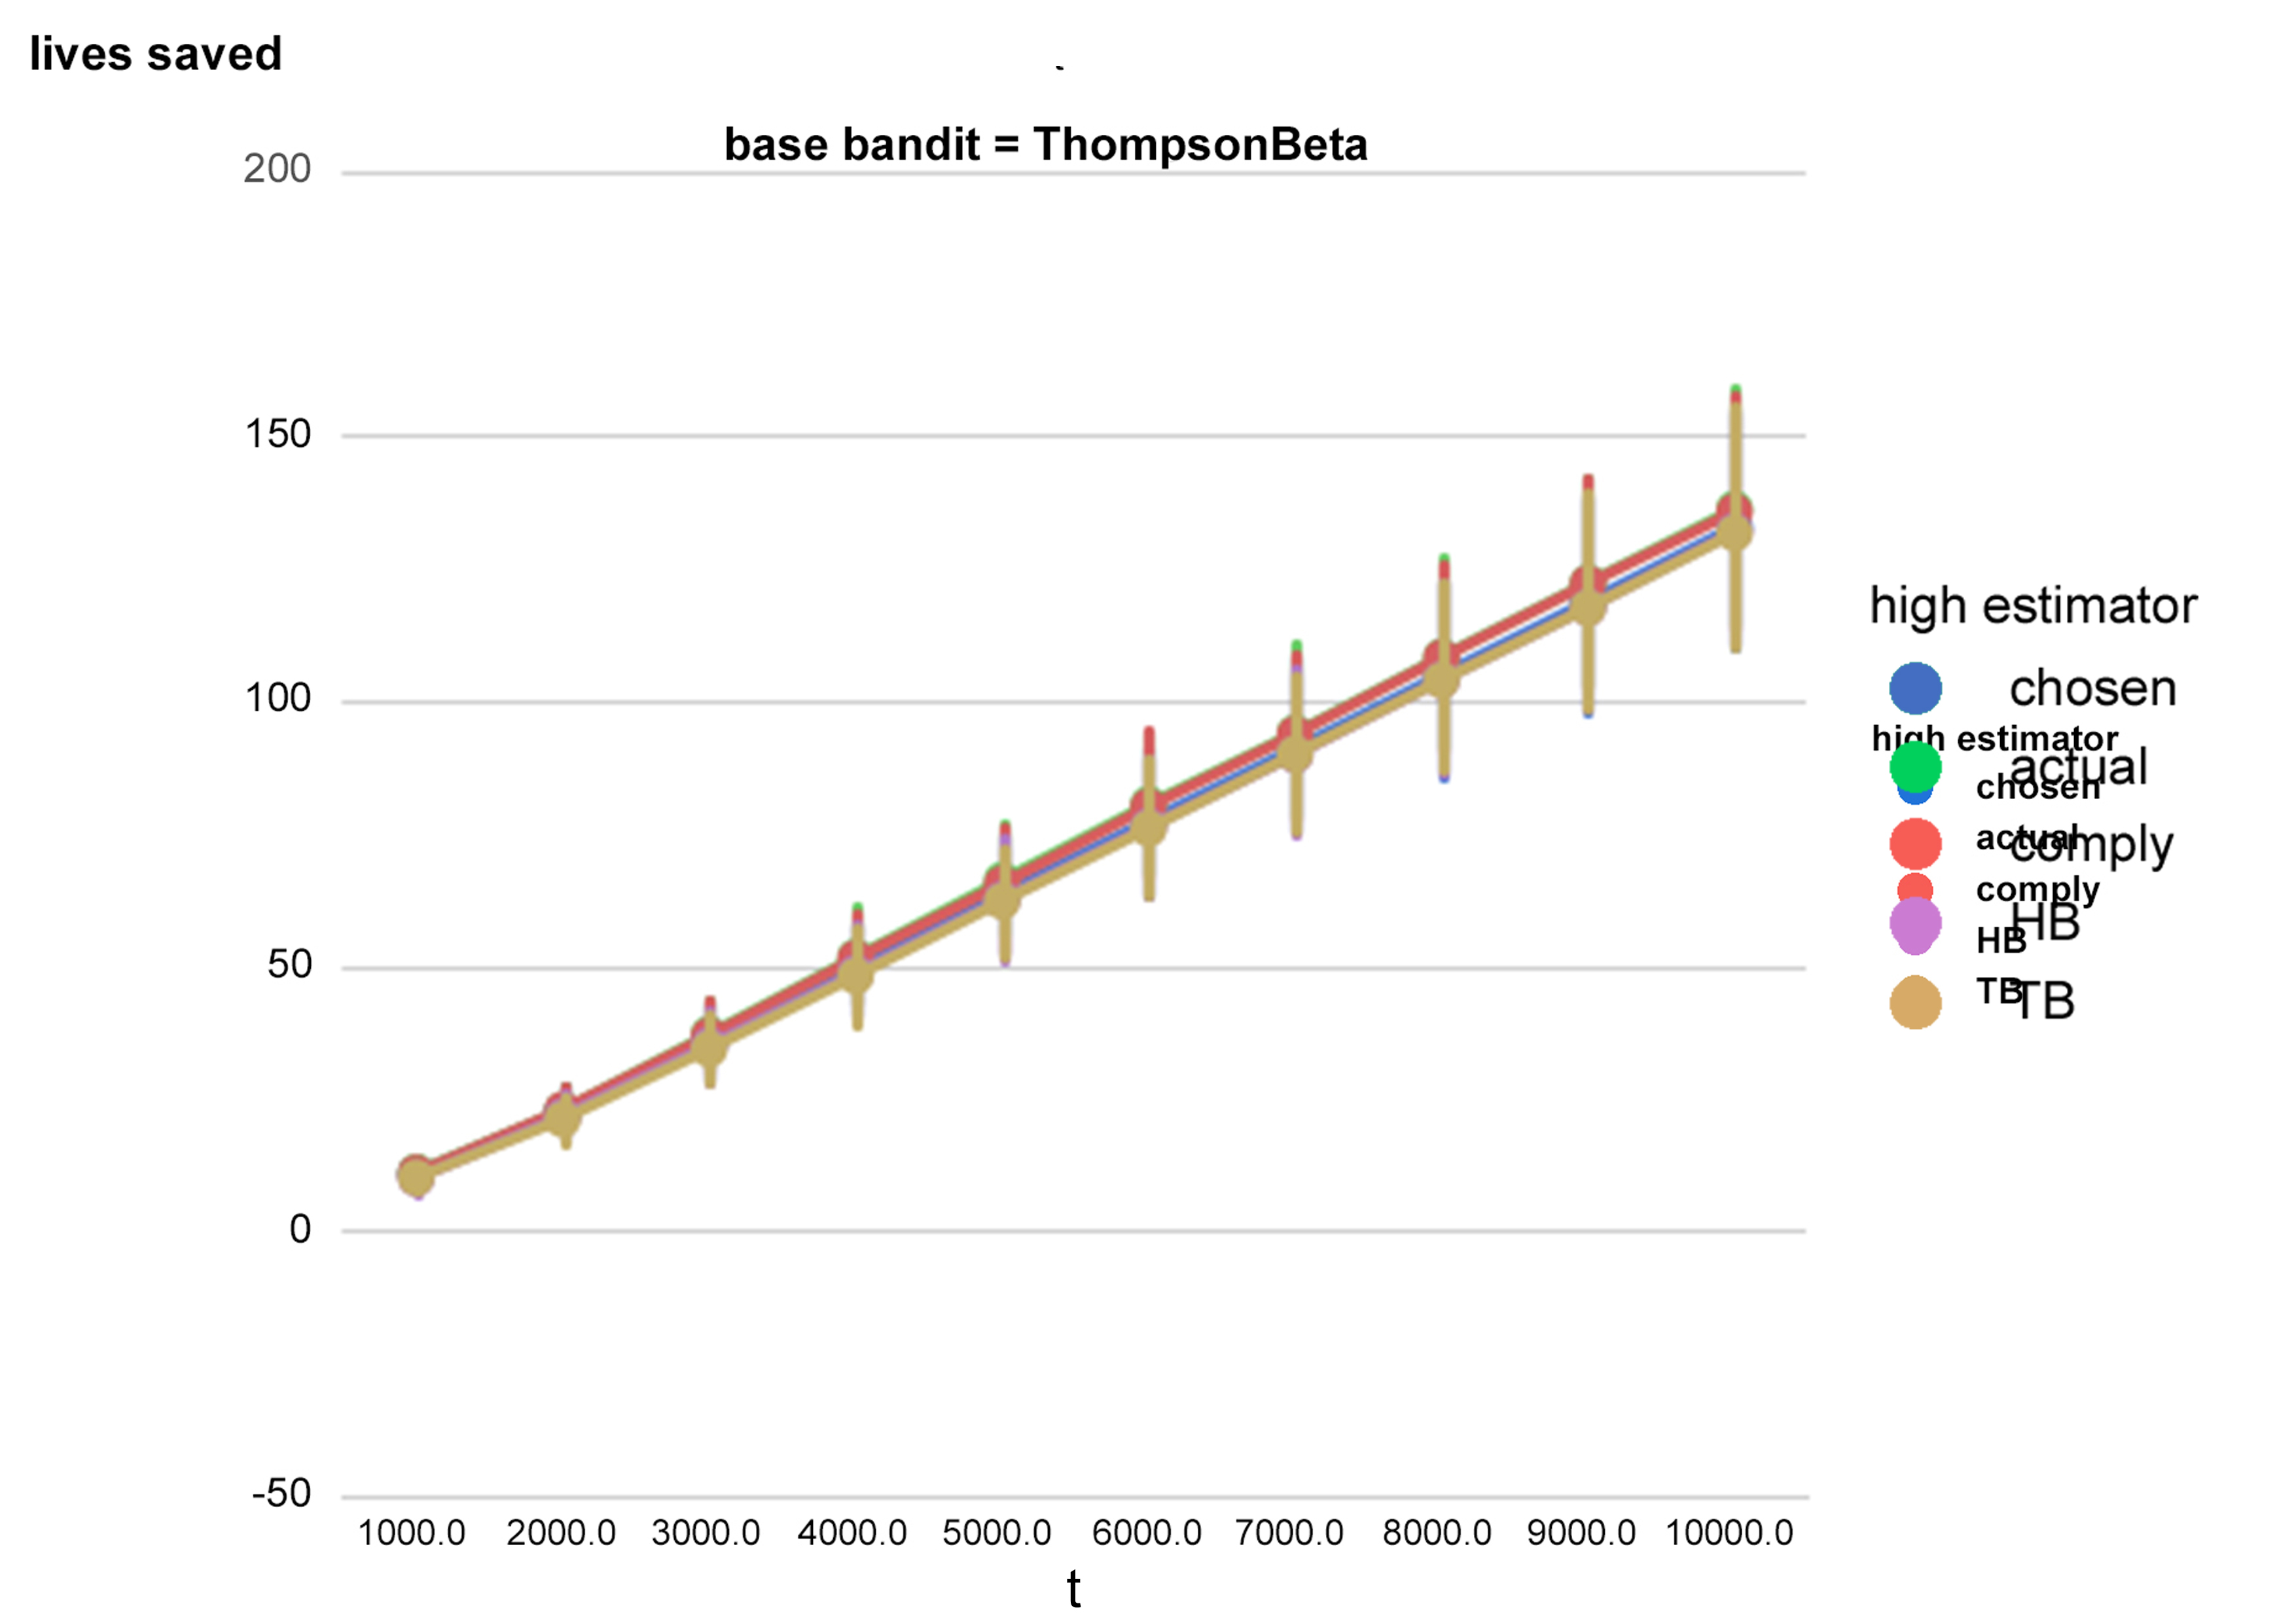
\includegraphics[width=0.9\textwidth]{bandit/figs/ex4-3.jpg}\hspace{1cm}
	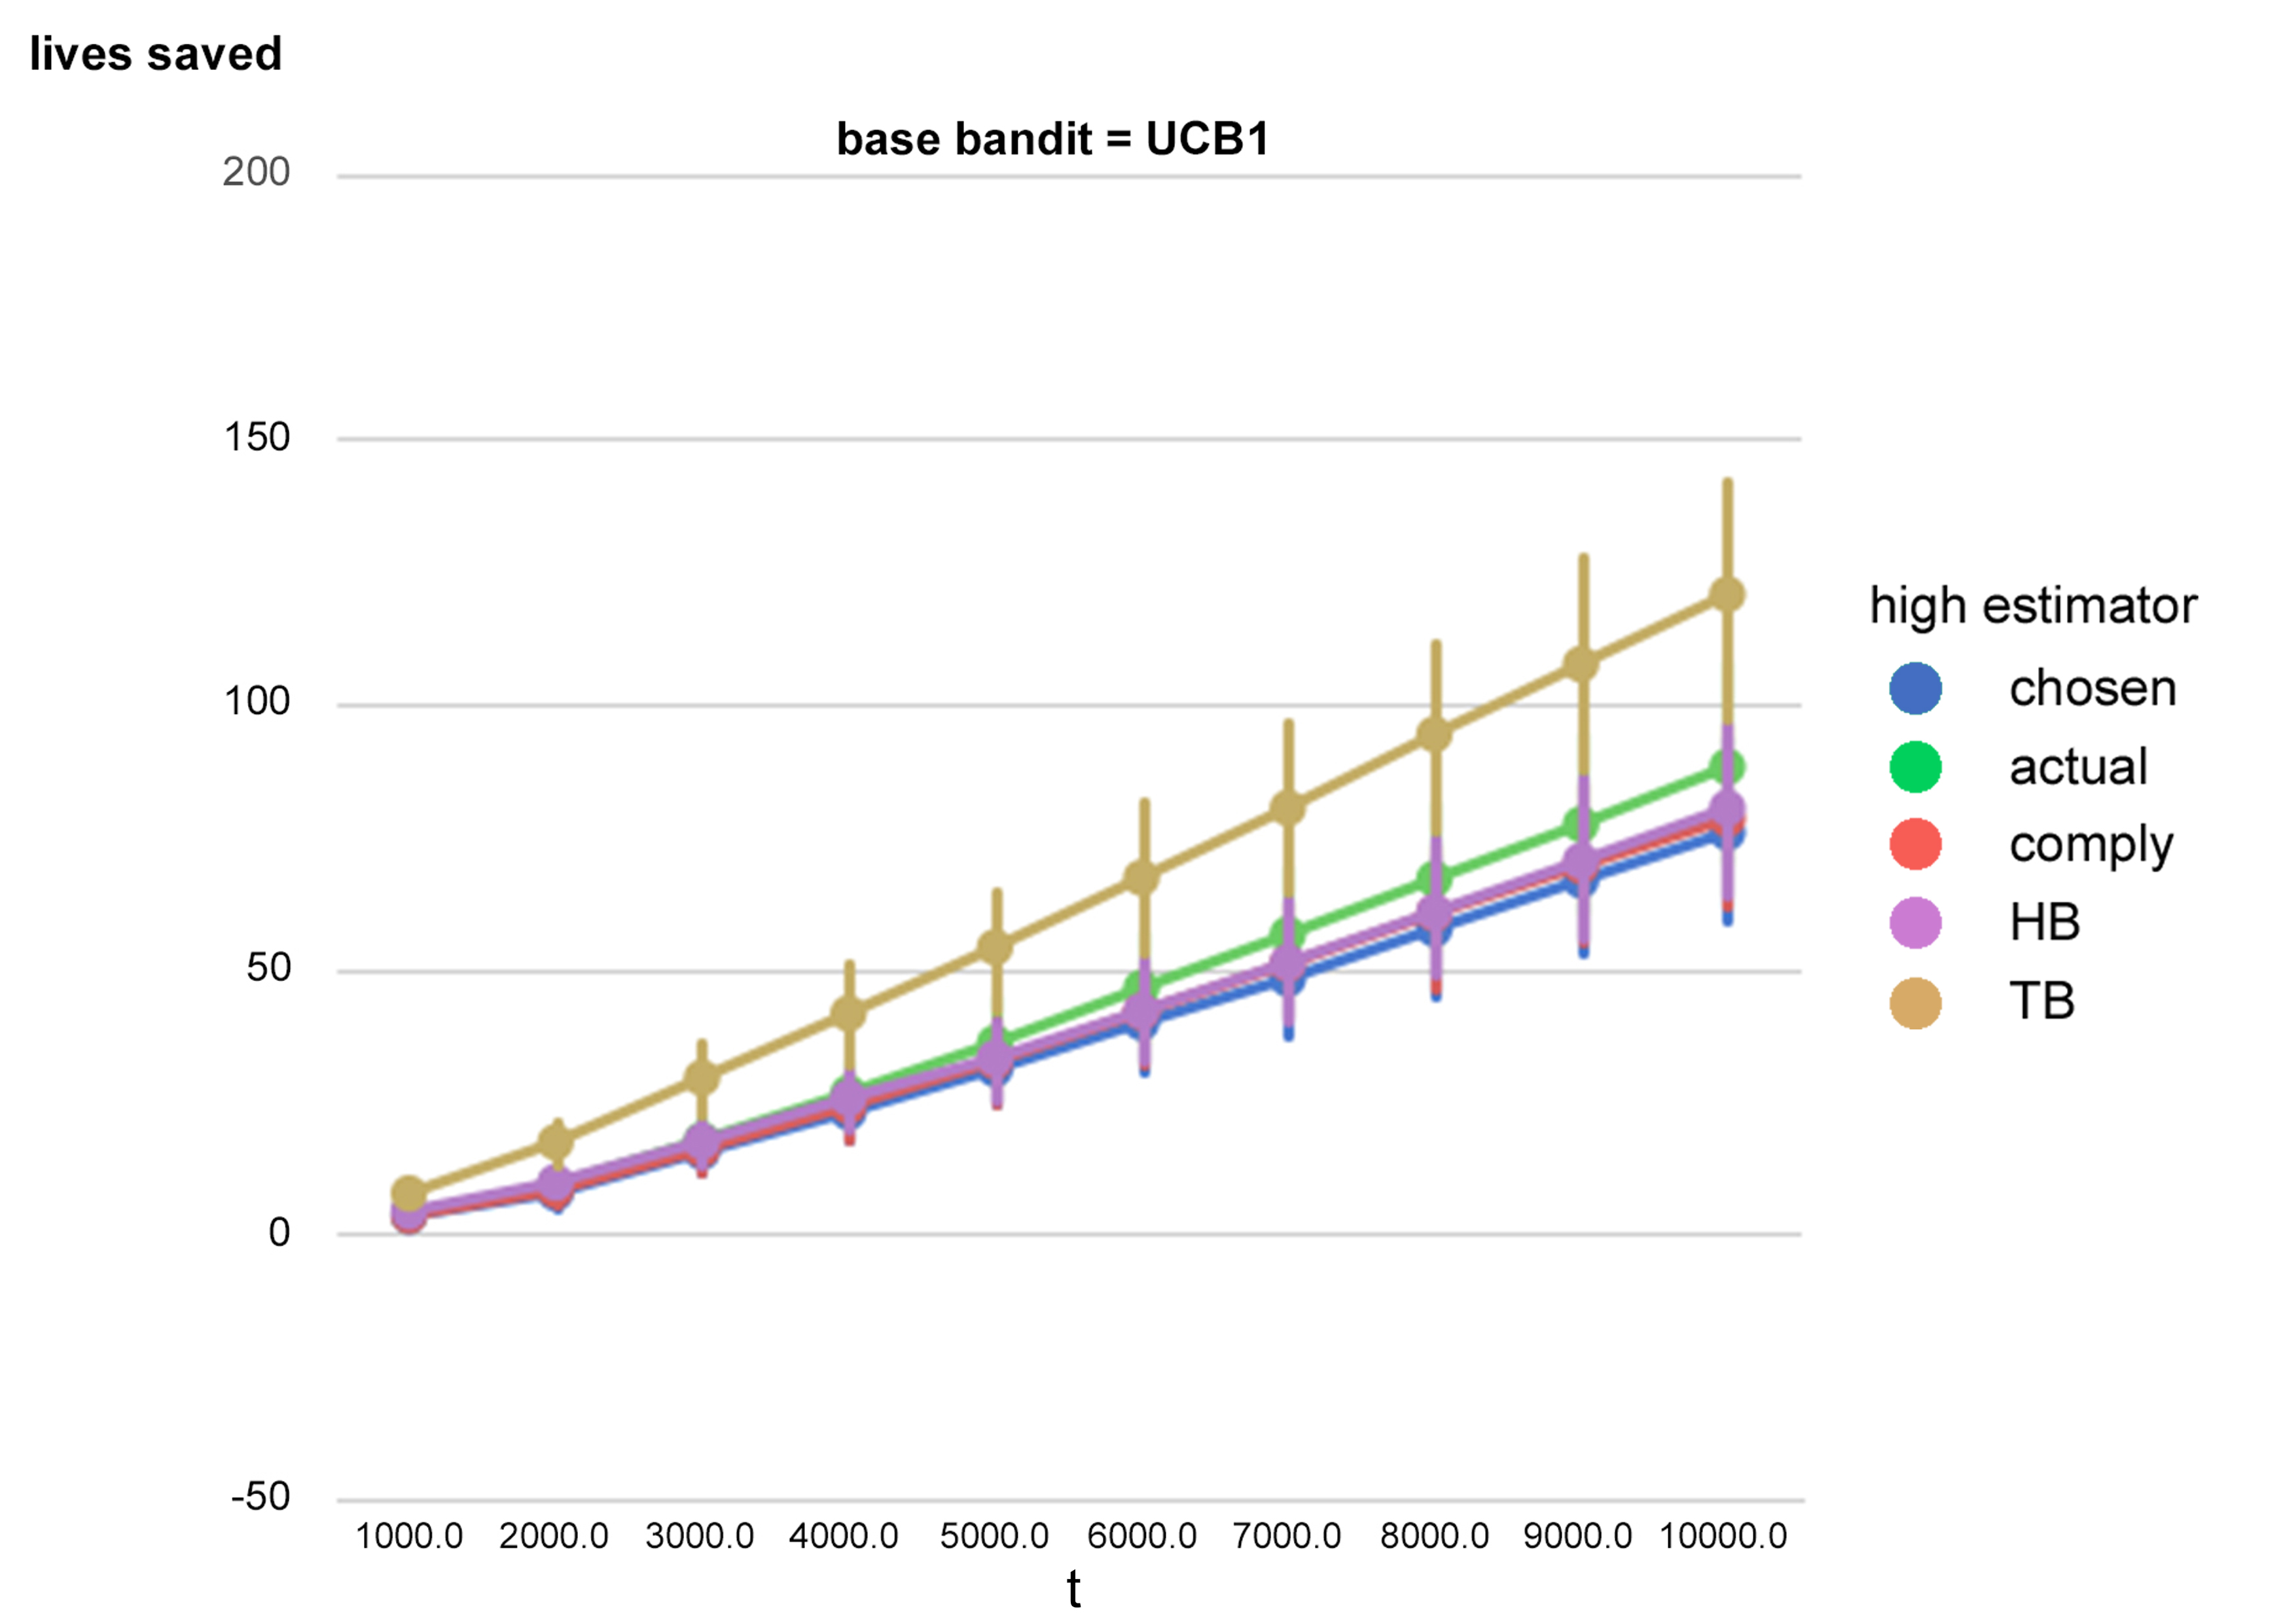
\includegraphics[width=0.9\textwidth]{bandit/figs/ex4-4.jpg}\hspace{1cm}
	\label{fig:ex4}
	\caption{Noncompliance for best arm: 100 simulations from synthetic data of $T=10,000$ with noncompliance proportional to how much better the best arm is than the algorithm selection.}
\end{figure}



%     def __init__(self,foo ):
%         n_arms=2
%         self.arm_value = 0.5+0.25*np.random.random(n_arms)
%         self.n_arms = n_arms
%     def draw_subject(self):
%         prefered_arm = stochastic_argmax(self.arm_value)
%         prefered_reward = random.binomial(1,self.arm_value[prefered_arm])
%         r = []
%         for i in range(self.n_arms):
%             if self.arm_value[i] / self.arm_value[prefered_arm] < random.random(): #informative noncompliance
%                 r.append((prefered_arm,prefered_reward))
%             else:  #compliers 
%                 r.append((i,  random.binomial(1,self.arm_value[i])))
%         return r

% example3= sim( nsim=100, T=10001, DGP=NoncomplianceForBestArm , drug="Better arm")
% display_results(example3.loc[example3['t'] == 10000].drop('t',1))



%\subsection{Independent Noncompliance and Rewards}

%We now simulate a neutral model, where compliance is unrelated to the rewards of the arm.
% #always or never takers. current simulation model is not rich enough for defiers, todo?
% class IndependentNoncomplianceAndRewards():
%     def __init__(self,foo):
%         n_arms=2
%         self.arm_value = 0.9+0.1*np.random.random(int(n_arms))
%         # todo add effect_magnitude=1
%         self.n_arms = n_arms
%     def draw_subject(self):
%         if random.random()<0.9: #compliers 
%             r=[(i, random.binomial(1,self.arm_value[i])) for i in range(self.n_arms)]
%         else:   #always takers
%             actual = categorical_draw(self.arm_value)
%             reward = random.binomial(1,self.arm_value[actual])
%             r= [(actual, reward) for i in range(self.n_arms)]
%         return r

    
% example4= sim( nsim=100, T=10001, DGP=IndependentNoncomplianceAndRewards , drug="example")
% display_results(example4.loc[example4['t'] == 10000].drop('t',1))







%think of the babies http://www.ncbi.nlm.nih.gov/pmc/articles/PMC2778326/



%We have two simulations, one in which noncompliance is independent of everything, and one where noncompliance is towards the higher expectation treatment.

%This is a boring figure, not rue what to say about it.
%%%%%%%%%%%%%%%%%%%%%%%%%%%%%%%%%%%%%%%%%%%%%%%%%%%%%%%%%%%%%%%%%%%%%%%%%%%%%%%%%%%%%%%%
%\subsection{Conclusions}

%Empirically, \texttt{TB} achieves a surplus of 8.9 extra survivals (that is, human lives) and \texttt{HB} achieves 9.2 surplus lives compared with 7.9 for the best classical algorithm. This suggests hybrid algorithms can make a significant difference to clinical outcomes.

% TODO, add note on composability and comparing to relatively well understood baselines. plug and play.




\part{Normative Implications for Mechanism Design: Advise Auctions}


\epigraph{Give the people what they want\\ when they want it \\
and they wants it all the time}{Parliament \\ Supergroovalisticprosifunkstication}

\chapter{Advice Auctions: Subject Freedom and Adviser Incentives for a Single Decision} \label{cha:market}

\section{Introduction}

%cahnnel from roth economist as enginerr
%Since then, economists have gained significant experience in practical market
%design. One thing we learned from this experience is that transactions and institutions %matter at a level of detail that economists have not often had to deal with,
%and, in this respect, all markets are different. But there are also general lessons.
%This essay will consider some ways in which markets succeed and fail by looking at
%some common patterns we see of market failures, and how they have been fixed."
%3. Make it safe to participate in the market as simply as possible, as opposed to
%transacting outside of the marketplace, or engaging in strategic behavior that	 reduces
%overall welfare.


This chapter considers a subject facing a decision, who wishes to incentivize multiple experts in providing advice so as to pick a decision that maximizes the rewards the subject receives, while maintaining the freedom of the subject.
Experts do not have intrinsic interest in the action the subject chooses or actually takes, nor do they face any costs in acquiring their signals.

Preserving subjects freedom is a inherently desirable practical design criterion as it enables no-regret exploration on the part of the subjects. Subject remains at all point in control of the decision, and so trying the mechanism cannot reduce their choices or their expected welfare.\footnote{One can set a reserve price of the advice auction to the expected value of the action the agent would have picked if they did not participate in the mechanism. As long as the reserve price is set apriori or alternative reports form the non-winning bidders are the only thing used to set it, the incentives do not change from those analized here.}.



The main contribution of this chapter is casting this setting as one of a single unit efficient allocation with interdependent valuations (\cite{milgrom1982theory,maskin1992auctions,ausubel1999generalized,mclean2004informational,roughgarden2016optimal,eden2018interdependent}).
This allows us to leverage existing results in that setting, which provide both necessary conditions for efficient allocations (single crossing conditions on the signal structure) and impossibility results when those are not met.

% Each bidder reports her type to the auctioneer. Given the reports, the auctioneer determines the allocation that maximizes surplus.
%The payment rule is the following extension of Vickrey auction pricing: a bidder is charged for a given unit that she wins according to valuations evaluated at the minimum signal that she could have reported and still won that unit.



The key conceptual contribution that allows this is to consider the allocation not over the decisions, but instead over the experts providing the advice. 
The item to be allocated is the right to observe the signal reports, provide the advice and a (linear) share of the reward obtained by the subject.
We term these mechanisms \emph{advice auctions}.
The term advice is chosen to highlight that the decision is not ultimately determined by the market, thus preserving the subject's freedom.
The term auction highlights that this procedure does not produce a sequence of prices through time.
It is this simultaneous nature that allows us to side-step the negative (from the perspective of freedom) results that constrain sequential mechanisms to having full support over actions in order to provide  incentives.

Sharing rewards after choosing what decision to advice is neither a pure private value (since the optimal choice conditional on information makes the value the same for everyone) nor pure common value (since the ability the select the optimal choice given access to the other signals might vary across agents).
A advantage of this framing as opposed to having a mechanism that directly outputs a chosen action is that it allows for the expert making the recommendation to have different influences on subject (i.e. some experts may be more persuasive).
If the mechanism output was a choice to advice the subject directly, we would have to restrict the expected reward the subject receives not to depend on which expert submitted which report, this can be seen as  a limit on subject freedom (since it it is an external constraint).
By having the mechanism select the expert instead of the choice,it also becomes natural to extend to the more practical setting that does not require the mechanism to have access to the valuation functions, but instead rely on the highest bidder to be able to aggregate reported signals effectively.

%This closely follows work on efficiency allocation with interdependent values , and our mechanism has the same two steps: first agents submit their signals so as to be able to determine the probabilities over states of the world, and the results of that are used to pick an efficient allocation in what is private .  


\subsection{Limits to Subject Freedom in Sequential Proper Scoring Rule Based Decision Markets}

One way to incentivize them is by applying the machinery of prediction markets based on sequentially shared proper scoring rules to the expected reward conditional on the action.
A challenge that presents itself is how to settle the markets for the reward conditional on the action which is not taken.
One natural approach is to void the trades in the markets for these actions, this being the originally proposed mechanism in this line of work \cite{hanson2002decision}, and only settling the markets where actions are taken.
While seemingly natural, this is not incentive compatible for the experts, even in the weak myopic sense, as shown in \cite{othman2010decision}. 

To understand why this is the case, consider a last trader facing the prediction market (sequential proper scoring rule)  where the  price is correct (matches the expected reward) for the optimal action but there is some other action that is misprinted. The profit maximizing move for this trader is to lower the price of the optimal action below the true price of the previously misprinted action, and correct the mispriced action to its true  price. 
The utility maximizing subject would then carry out the suboptimal action, the expert would be rewarded for correctly predicting it and would receive no punishment for the error they introduced into the reward of the optimal action. 
%A mechanism is called Bayes Nash Incentive Compatible (BNIC) if there is a equilibrium were every agent reports their signal truthfully and this maximizes their reward in expectation (over the state of the world).
The mechanism proposed in \cite{hanson2002decision} is not BNIC for the experts who provide advice, as witnessed by the example above (and shown in \cite{othman2010decision,chen2014eliciting}).
More generally, any sequential proper scoring rule based mechanism that is incentive compatible for the experts is incompatible with maintaining the subject's freedom to select the action that appears optimal ex-post (\cite{ chen2014eliciting}). 

%Interdependent Values without Single-Crossing
%Alon Eden, Michal Feldman, Amos Fiat, Kira Goldner
%We consider a setting where an auctioneer sells a single item to n potential agents with {\em interdependent values}. That is, each agent has her own private signal, and the valuation of each agent is a known function of all n private signals. This captures settings such as valuations for artwork, oil drilling rights, broadcast rights, and many more. 


%In the interdependent value setting, all previous work has assumed a so-called {\sl single-crossing condition}. Single-crossing means that the impact of agent i's private signal, si, on her own valuation is greater than the impact of si on the valuation of any other agent. It is known that without the single-crossing condition an efficient outcome cannot be obtained. We study welfare maximization for interdependent valuations through the lens of approximation. 


%\cite{eden2018interdependent}
%We show that, in general, without the single-crossing condition, one cannot hope to approximate the optimal social welfare any better than the approximation given by assigning the item to a random bidder. 
%Consequently, we introduce a relaxed version of single-crossing, {\sl c-single-crossing}, parameterized by c≥1, which means that the impact of si on the valuation of agent i is at least 1/c times the impact of si on the valuation of any other agent (c=1 is single-crossing). Using this parameterized notion, we obtain a host of positive results. 


% The first step of our procedure maps to the setting of 
% https://www.sas.upenn.edu/~apostlew/paper/pdf/auctionrevised.pdf
%and more generally
% TE2015 



\subsection{Summary and Outline}

%TODO: garrett says more clear explanation. make explicit pointer to background section, and make paragraph of sentence.
%The core of the problem which emerges upon using the machinery of prediction markets in the decision setting is that

The rest of the chapter is structured as follows.
We first introduce a formal model and notation.
We then present advice auctions as a direct mechanism, show when they are truthful, as well as their limits.
We then consider two practical indirect variations of the procedure, which removes the need for the mechanism to have any knowledge of valuations, and consider sufficient conditions for their efficiency and truthfulness.  



\section{Model}



As before, the subject seeks advice on a decision they will take from some finite set of alternatives $A$, let $c$ be the choice that is given as advice to the subject and $a$ the decision that the subject actually takes.
The rest of our model and notation largely follow that of \cite{eden2018interdependent}.%\footnote{Relative to their notation and to maintain coherency with the other chapters in the thesis, in our setting the number of potential actions is $q$ instead of $k$, while  }.
Each expert $i \in \{1, \ldots, n\}$ receives a single signal $s_i$ which is known only to expert $i$.
Potential signals for bidder $1 \leq i\leq n$ form a discrete signal space $S_i$.
Let $\vec{s}=(s_1,s_2,\ldots,s_n)$ be a signal profile.
The reward $r$ that the subject receives depends on their chosen action $a$ and the underlying state of the world as determined by the signal profile $\vec{s}$.
Let $\vec{s}_{-i}$ denote all signals but $s_i$, and let $(s_i',\vec{s}_{-i})$ denote the profile $\vec{s}$ where $s_i$ has been replaced with $s'_i$. 
Since $r$ does not depend on the choice of $c$ by the expert, and that at the point the mechanism is run $a$ has not been selected, we use the following reduced form  value function for the value of the rights bundle to expert $i$: $v_i: \times_i \ S_i \rightarrow \mathbb{R}_{\geq 0}$, which maps every signal profile to the expected value of linear share of the reward  $\alpha r$.


Each expert reports a signal $b_i$, and the vector of reported signals is $\vec{b}=( b_1, b_2, \ldots, b_n)$.
Each possible signal profile $\vec{s}$ corresponds to an underlying state of the world, this includes both inherent physical properties of the subject and the actions, as well as the subjects probability of choice of $a$ in response to different choices of $c$.
%Without loss of generality, assume $S_i=\{0,1,\ldots,q_i\}$.


%This value is given by $\alpha r(\vec{s})$
The valuation functions for all bidders $i$ are monotone non-decreasing in every signal $s_j$ for all $j$.%\footnote{Both of these assumptions are without loss of generality; the space of potential signals can alwyas be , while the ordering of the signals is arbitrary, so they can always be sorted into monotone non-decreasing.}

Mechanisms are a pair $(x,p)$, where $x$ is a set of allocation functions $x=\{x_1(\vec{b}),\ldots,x_n(\vec{b})\}$ satisfying $\sum_i x_i(\vec{s}) \leq 1$ for all possible $\vec{b}$, and $p$ a set of payment functions  $p=\{p_1(\vec{b}),\ldots,p_n(\vec{b})\}$.
An allocation function $x_i:\times_j \ S_j\rightarrow [0,1]$ maps every bid profile $\vec{b}$ to the probability that expert $i$ gets allocated.
A payment rule $p_i: \times _j S_j \rightarrow \cR$ maps the reported signals $\vec{b}$ to the expected payment from bidder $i$. Experts are risk neutral, so their expected utility is quasilinear, given in the reduced form by $x_i (\vec{b}) \cdot v_i(\vec{s}) - p_i(\vec{b})$ where $\vec{s}$ is the true signal profile of the experts.


%One cannot hope for truth-telling to be a dominant strategy for the experts. One expert's misreport can cause other experts to also misreport to compensate. Thus the strongest incentive-compatibility (IC) notion that we can hope for is in this setting is truthfulness is an ex-post Nash Equilibrium. That is it is in every agent $i$'s best interest to report his true signal $s_i$ given that all other agents reported the true signal profile $\vec{s}_{-i}$:
$$x_i(\vec{s}) \cdot v_i(\vec{s}) - p_i(\vec{s}) \geq x_i(b_i, \vec{s}_{-i}) \cdot v_i(\vec{s}) - p_i(b_i, \vec{s}_{-i})  \quad \quad \quad  \forall \vec{s} \in \times _{j} \  S_j, b_i \in S_i. \quad\quad\quad [\text{IC}]$$




%As in \cite{mclean2004informational} an experts  information may be of two qualitatively different kinds: information about the objective characteristics of the subject and the effects of their alternative decisions and how generally persuasive they are to find the recommended action.
%Idiosyncratic information about the agent himself: their ability to aggregate the signals efficiently, and how persuasive the would result as the advisors who selected $c$ in the second stage of the game. 
%The former is of interest to other agents—and consequently is the cause of the interdependence of agents’ values—while the latter is irrelevant to other agents in calculating their values.


\section{A Direct Reward Sharing Mechanism}

The simplest class of mechanisms to incentivize advice is based on sharing a fraction of the rewards with the experts. For the single expert case this is mentioned by \cite{othman2010decision}. Here the idea is extended to the multiple experts case. We do this by instantiating our notion of advice auctions with a simple mechanism,
the generalized VCG mechanism proposed by \cite{maskin1992auctions}. This mechanism is \emph{direct} in the standard sense that agents report their signals. 

The core of the mechanism is simple. Since there is knowledge by the mechanism over the value function for a given vector of signals, it can use the reported signals to select the highest value expert. The net payment to that expert is then just his share of the reward minus his value at the lowest signal he could have misreported and still obtained the allocation give the other reports. More formally:

\begin{mech}\label{mech:Direct}[Direct Reward Share VCG]
Then mechanism gives the rights bundle to the expert $i^*$ with the highest valuation under the reported signals. That is, the allocation rule is:

$$x(\vec{s}) = i \quad \quad\quad \text{when} \quad\quad\quad x_j(\vec{s}) = \begin{cases} 1 & \text{if } j=i \\ 0 & \text{otherwise.} \end{cases}$$

This lets the expert $i^*$ observe  $\vec{b}$ and then select $c$.
Then subject observes $c$ and $\vec{b}$, takes their action $a$ and receives reward $r$, which the mechanism observes. 

The non selected experts receive no payment, while the selected expert $i^*$ receives their share $\alpha$ of the reward $r$ minus the value of the share of the reward at the lowest $b_i'$ (the critical signal) that would have still resulted in expert $i$ being selected. 
More formally, given signals for agents $\neq i$, $\vec{s}_{-i}$, the {\sl critical signal} for $i$ is: if there exists some $b_i$ such that $x_i(s_{-i},b_i)=1$ then set $b_i^*=\min_{b_i} x_i(s_{-i},b_i)=1$, otherwise there is no critical signal for $i$.
Thus, the payment rule is:

$p_i= \alpha r - v_i(\vec{s}_{-i},b_i^*)$

\end{mech}

An allocation function $x_i$ is called {\sl deterministic} if $x_i(\vec{b})\in \{0,1\}$ for all $i$ and all $\vec{b}$.
The generalized direct VCG mechanism is deterministic and prior-free.

\subsection{Truthfulness with Single Crossing Signals}

\begin{defn}[Monotonicity]
	An allocation function $x_i$ is said to be monotone if for every $\vec{b}_{-i}$, $x_i(\vec{b}_{-i},b_i)$ is monotone non-decreasing in the signal $b_i$.
\end{defn}

Truthful mechanisms can be characterized as follows \cite{roughgarden2016optimal}.

\begin{prop}\label{prop:char-ic}
	Monotonicity is a necessary and sufficient condition for allocation functions $x$ to be \emph{implementable}, {\sl i.e.}, there exist payment functions $p$ such that the mechanism $(x,p)$ is truthful.  Moreover, an analogue of Myerson's payment identity holds, so the payment is uniquely determined by the allocation function.
\end{prop}

It follows that constructing a truthful mechanism is equivalent to constructing a monotone allocation function.
For deterministic truthful mechanisms, the payment identity of \citet{roughgarden2016optimal} implies the following about the cost charged to a chosen expert (from \cite{eden2018interdependent}).

\begin{prop}\label{prop:deterministic_payment}
	Let agent $i$ be the allocated winner at report profile $\vec{s}$ in a deterministic truthful mechanism. Then their cost is their value at the critical report.
\end{prop}


A single-crossing condition captures the idea that bidder $i$'s signal has a greater effect on experts $i$'s value than on any other experts's value. We follow the definition in \cite{eden2018interdependent}:

For $s_i = 1, \ldots, k_i$, define $\frac{\partial v_j(s_i, \vec{s}_{-i})}{\partial s_i} = v_j(s_i, \vec{s}_{-i}) - v_j(s_i - 1, \vec{s}_{-i})$.

\begin{defn}[Single-Crossing]
	A valuation profile is said to satisfy the single-crossing condition if for every expert $i$, for any set of other experts  signals $\vec{s}_{-i}$, and for every expert $j$, $$\frac{\partial v_i(s_i, \vec{s}_{-i})}{\partial s_i} \geq \frac{\partial v_j(s_i, \vec{s}_{-i})}{\partial s_i}.$$
\end{defn}


%We note that there also exists a weaker notion of single-crossing that only requires the inequality to hold at $\vec{s}$ for the bidder $i$ with the highest value, where $i \in \argmax_{k} v_k(\vec{s})$.

\begin{thm}
	There is a truthful and efficient ex-post Nash equilibrium of the DRSA mechanism when signals satisfy the single crossing property.
\end{thm}

\begin{proof}
Allocating to the bidder with the highest value is a monotone allocation rule, and therefore, according to Proposition~\ref{prop:char-ic} it is implementable. The cost for the rights bundle of the chosen expert is then just their value at their critical signal, which is the corresponding payment.
\end{proof}

Further, one cannot do better than this as per Proposition~\ref{prop:char-ic}, monotonicity of the allocation rule is necessary for a efficient and truthful mechanism with interdepedent values. Hence, without single-crossing, it is impossible to have a truthful advice auction in general.

This procedure for a direct advice elicitation mechanism based on the advice auction procedure was here instantiated using \cite{maskin1992auctions}  as the underlying auction mechanism. But the procedure is generic. It could be, for example, instantiated instead with the randomized mechanism of \cite{eden2018interdependent}, and would obtain the approximation properties that algorithm provides in auctions in our advice setting.


\section{Practical mechanisms: Advice Auctions}

The assumptions used in \cite{roughgarden2016optimal} that are used for the above result are extremely minimal relative to the existing literature in most of decision markets and auctions with interdependent values.

However, the mechanism having access to the value functions seems highly impractical in most potential applications.
Given the practical settings that motivate this work, 
we do not assume access by the mechanism to a the valuation functions, and consider two practical alternatives.


\subsection{A Bid and Signal Reward Sharing Mechanism}

The first modification one can do to make the payment of the highest bidder depend on the bid of the second highest, this removes the dependency of the payments function on the 
valuation functions of experts.
The challenge this faces is that the signals reports being submitted would not matter, so any signal report is in equilibrium. To correct this and restore strict incentives, we can add a further payment received by all experts that is also a linear share of the reward (denoted by $\beta$). This makes the truthful signaling equilibrium potentially strict.


\begin{mech}\label{mech:Direct}[Allocation with Bids, Reward Share with Signals (ABRSS)]
	Experts report both a bid and a signal, we slightly abuse notation and use $vec(s)$ to denote the reported signals, note their only use is to be displayed to the expert allocated to make the choice..
	Then the mechanism gives the rights bundle to the expert $i^*$ with the highest bid:
	
	$$x(\vec{b}) = i \quad \quad\quad \text{when} \quad\quad\quad x_j(\vec{b}) = \begin{cases} 1 & \text{if } j=i \\ 0 & \text{otherwise.} \end{cases}$$
	
	This lets the expert $i^*$ observe reported signals $\vec{s}$ and select $c$.
	Then subject observes $c$ and $\vec{b}$ and $\vec{s}$, takes their action $a$ and receives reward $r$, which the mechanism observes. 
	
	The non selected experts receive  payment $\beta r$, while the selected expert $i^*$ receives their shares $(\alpha + \beta) r$ of the reward minus the second highest bid, $b_{i^*-1}$.

	Thus, the payment rule is:
	
	$p_i^*= ((\alpha + \beta)r - b_{i^*-1})$ and $p_{j\neq i^*} = \beta r$
\end{mech}



For this allocation rule to reach efficient allocation achieved by the direct mechanism, a stronger assumption on signal structure is needed. If we only require single crossing then the identity of the highest valuation expert can depend on interaction of their signals and those of other experts. Without access to the value function the mechanism cannot in general hope to achieve this allocation.
Thus beyond single crossing, we also require that the highest valuation expert must be so for any possible set of signals other than their own. In this case the allocation of this mechanism is efficient, since it coincides with the direct mechanisms allocation.

%MORE FORMALY

\begin{defn}[Single Signal Max Value]
	A valuation profile is said to satisfy the single-signal max value condition if highest value expert $i^*$ knows he is the highest value when given their signal, and for any set of other experts  signals $\vec{s}_{-i}$, and for every expert $j$: $$v_i(s_i, \vec{s}_{-i}) \geq  v_j(s_i, \vec{s}_{-i})$$
\end{defn}


Note this property is not as strong as it may at first seem. If there is an expert who has the trust of the subject, understands what they find persuasive, and is sufficiently competent at evaluating the reported signals of others, it may be best able to select $c$ to maximize $r$ no matter the state of the world. Being able to see other experts' signals may however substantially raise the reward and hence the value of the highest valued expert.  


\begin{thm}
	There is a truthful and efficient ex-post Nash equilibrium of the ABRSS mechanism when signals satisfy the single signal max value property.
\end{thm}

\begin{proof}
	The highest value bidder bids his worst possible value given the other bids or anything higher (knowing he will win and be charged according to the second highest price makes him indifferent between these when others are truthful).
	Allocating to the bidder with the highest value is a monotone allocation rule, and therefore, according to Proposition~\ref{prop:char-ic} it is implementable. The cost for the rights bundle of the chosen expert is then the second highest bid, which is the corresponding payment.
\end{proof}



For contrast consider the identical mechanism but without the experts submitting their signals and receiving share $\beta$. 
 
\begin{mech}\label{mech:BidOnly}[Bid Only Advice Auction]
 	Each expert observes their signal and then report only a bid $b_i$. The mechanism gives the rights bundle to the expert $i^*$ with the highest bid:
 	
 	$$x(\vec{b}) = i \quad \quad\quad \text{when} \quad\quad\quad x_j(\vec{b}) = \begin{cases} 1 & \text{if } j=i \\ 0 & \text{otherwise.} \end{cases}$$
 	
 	This lets the expert $i^*$ observe reported bids $\vec{b}$ and then select $c$.
 	Then the subject observes $c$ and $\vec{b}$, takes their action $a$ and receives reward $r$, which the mechanism observes. 
 	
 	The non-selected experts receive  payment $\beta r$, while the selected expert $i^*$ receives their shares $(\alpha + \beta) r$ of the reward minus the second highest bid, $b_{i^*-1}$.
 	
 	Thus, the payment rule is:
 	
 	$p_i^*= ((\alpha + \beta)r - b_{i^*-1})$ and $p_{j\neq i^*} = \beta r$
 \end{mech}
 
 For some very limited information structures the bidding mechanism still aggregates information efficiently. 
 These information structures correspond to the standard private values settings in which the Vickrey auction is efficient \cite{vickrey1961}.
 Private values occur when other experts signals are not informative of the value for an expert of being assigned the rights bundle to make the choice.
 For example, when each expert signal is only informative about the expected outcome conditional on one action, and  there is one expert who is informed about each action.
 
 
 This kind of indirect mechanism is inherently limited when the value from the signals of experts are interrelated (as we proved before). Their bid, cannot encode the full information contained in the signals, and thus this limits any mechanism that relies solely on single rounds of bids to aggregate information.
 
 To illustrate this consider a setting that satisfies the single max bidder assumption. Denote by $i^*$ the experts whose valuation is higher than all other experts in every state of the world and who knows the subject trust them completely so if he wins $c=a$. Have a second expert whose value is $0$ in all state of the world\footnote{For example the expert might know the subject is biased and refuses to hear the expert due to color of their skin.} but has a binary independent signal $s_{treat}$ that determines which choice is best for the subject, without knowing $s_{treat}$ the two best choices have equal expected reward $r_{uniform}$, while knowing the value of the signal allows to select the appropriate choice and results in double the reward $2r_{uniform}$.
 Since their value for the rights bundle is always 0, thus their bid is in equilibrium. 
 There is no prior-free way for the unpersuasive expert to encode his signal into their bid (even through he is incentivize to reveal their signal to get a higher $\beta$ payment). 
 Notice that there is no limit in the size of the gap in the rewards between the two allocations in general, as in the example above we can replace $2$ by any number.
 
 

\section{Conclusion}

This chapter shows how to use the bundle of rights perspective on advisers to recast the incentivizes for decision elicitation from multiple experts into the thriving literature on VCG with interdependent valuations.
We then use a result of \cite{roughgarden2016optimal} for the generalized VCG mechanism of \cite{maskin1992auctions} to allocate the rights results in a direct incentive compatible and efficient mechanism when signals have a single crossing property.
We then explore two practical variations of the mechanism that relax the assumption that the mechanism can access the value functions of experts, and that signals can be transmitted between experts. We give sufficient conditions on the structure of the signals so that the variations of the mechanisms preserve truthfulness and efficiency.


\chapter{A General Setting and a First Approach} \label{cha:twosided}
%We consider a natural setting that generalizes both previous models.
%!TEX root = main.tex

\subsection{Introduction}

This chapter differs from the previous ones in its relationship to the thesis. 
While before we seek to extend the understanding of previously presented settings (bandit algorithms and decision markets), this chapter seeks to introduce a new setting that generalizes these two.



Our motivating applications in medicine suggest a sequence of similar decisions faced by a sequence of agents in order, all of whom face an individual choice on their own course of action.
Every day new patients perceive their symptoms, and they seek diagnoses and treatments from medical providers. Other applications are conceivable:
A corporation faces new investment opportunities with regularity, and similar opportunities appear to many firms that might not be competitive (for example vertical divisions in a conglomerate might be offered similar projects to automate part of their workflows and must choose whether to attempt them or not. They might be able to ask their inhouse experts for advice on the right course of action).
Scenarios such as these that motivate optimal decision elicitation are in a sense naturally cast not as one-shot interactions, but as repeated games with many experts and a sequence of subjects who seek advice before making a decision which only affects them.

This combines the central aspects of bandits with compliance awareness (a sequence of choices and learning from past experience, where the actions of subjects are not bound to follow the algorithm choice) as well as elicitation of information from experts to enable optimal decisions without the advice being binding. 



The study of decision markets so far, including the previous chapter, has focused on a setting with a single decision and multiple advisers (\cite{hanson2002decision,othman2010decision,chen2014eliciting}).
This chapter poses a novel and natural generalization of this setting that also captures the compliance aware bandit setting and the advice auctions as special cases. 
We consider a sequence of $T$ subjects (patients in the medical motivation), and a fixed set of $K$ advisers (experts) with access to signals about different patients' expected rewards $r$ under different advice $c$ and actual courses of action $a$. 
The bounded regret algorithms with compliance awareness introduced in Chapter 3 can be seen as addressing the special case where the experts' signals are known a priori to be uninformative, so $K=0$ effectively, and thus only the experience can be learned from.
A situation where experts always report their signals truthfully and have no knowledge over how to aggregate them beyond that possessed by the mechanism is equivalent to a compliance-aware contextual bandit problem. 
When contexts are constant across all time steps, the situation further reduces to a bandit problem with compliance awareness.
When the subject always follows the mechanism or $a$ cannot be observed, it reduces further  to the standard multi-armed bandit problem. 
Our one-subject mechanism in Chapter 5 is the special case for $T=1$, thus there is no role for exploration or learning from experience, since there are no future decisions to help inform.


In contrast to the previous chapters' motivation in the literature, in this chapter our focus is first and foremost on constructing a practical mechanism. 
The reason for this switch is that the setting is natural, and no mechanisms (nor the setting itself) have been previously proposed to the best of our knowledge.
The most conceptually interesting possibility when moving to a sequence of $T$ agents is that it can be ex-post incentive compatible to take the exploratory actions for subjects, by linking them to suitably large transfers. By introducing randomness into which subjects and which actions have these transfers attached, and into their magnitude, it becomes possible to estimate the underlying causal effect of actions on rewards. 

%In the two special cases of compliance aware bandits and single subject decision markets, the proposed mechanism reduces to the previously proposed mechanism.
%There are, however, infinite other mechanisms that share this property. 

%This source of endogenous heterogeneity in ex-ante identical agents rewards and incentives to take different actions can also be leveraged to evaluate 



We build up to the main practical design by analyzing two simplified models that illustrate the two key characteristics of our mechanism. 
The first is the need for incentives to motivate exploratory choices.
For this, the rewards from the choice of action must be linked not just to the reward during the period in which the action is taken, but to the full sequence of subsequent future rewards.
Second, to aggregate signals when single crossing conditions and their approximations are violated, we propose using an off-line contextual bandit algorithm to evaluate the counter-factual (marginal) value of the signals each expert provides.
We present a mechanism that combines both ideas, and explore some of its limitations.



\section{Model}

The game occurs over $T$ steps. At each step: 

\begin{enumerate}
\item A new subject $t$ arrives and each $i$ of $K$ experts receives a signal $s_{t,i}$ for that subject. The mechanism  randomly allocates a contingent transfer payment of $\vec{\gamma_t}$ for each of the possible actions facing the subject. %TODO what is a transfer payment?
\item Each expert $i$ reports ${b}_{t,i}$ to the mechanism. After all reports are received, the mechanism selects an expert $i^{*}$ to suggest an action $c_t$.
\item The subject observes $c_t$, $a_t'$ and ${b}_{t,i}$, picks an action $a_t$, and receives a reward $r_t$. %TODO what is a_t'?
\item The mechanism provides feedback about $s_t$, $c_t$, $a_t$, and $r_t$ to experts. %TODO do you mean \vec s?
\end{enumerate}

At the end of the final period the mechanism makes payments $p_i$ to the experts.


\subsection{Subjects' Beliefs and Incentives}


Previous work on incentive compatible bandits \cite{kremer2014implementing,mansour2015bayesian} has shown that there are distributions of rewards where if all agents were rational and this was common knowledge, some actions can never be explored (assuming only information revelation and no transfers can be used by the mechanism). 
Namely, actions that a priori have lower expected rewards than all others no matter what is revealed by previous instances of other actions cannot be explored.
The logic behind this is that knowing no previous signal could persuade an agent to take the action, an agent told to take the action knows that in expectation they can do better.
That literature has largely been focused on finding information revelation strategies that are optimal, subject to the incentive constraints. 
Our lottery payments allow us to side step these impossibility results, by providing a reason for exploration for a individual subject. 

%A closely related assumption (for the setting without outside experts providing advice, but with other agents also participating in a game with joint payoffs \cite{mansour2016bayesian}) are \emph{explorable actions}: the actions which some incentive-compatible policy can recommend with non-zero probability. Note that by making beliefs that there are other agents who are likely to take any actions sufficiently often enough to reveal if the rewards of that action are of the highest value, all actions can become explorable.


%The motivation behind this choice is that in many settings it is natural that the experts are playing the game repeatedly and for profit, thus rationality can be naturally achieved and sustained; this is much less likely to be the case for the subjects.
%\footnote{Ample evidence from experimental economics shows that while humans in unfamiliar environments can be far from rational, experienced professionals faced with similar real world tasks are much likelier to be rational, and this common knowledge. A vivid illustration of this is provided by experiments where chess players are faced with a centipede game.}
%It is precisely because subjects are in an unfamiliar situation that they seek out the help of experts in making their decisions.

%The model's main concern is thus in contrast to (\cite{kremer2014implementing,mansour2015bayesian}), who take the subjects as rational and the mechanism as the social planner which learns from experience, without relying on information from rational experts.
%While the assumption of rationality and common knowledge in that case enable the use of information revelation structures for incentive exploration, here we take the exploration for granted and focus on the incentives of the experts.

\section{A sequence of repeated one-shot-efficient mechanisms is inefficient}

One could attempt running the direct mechanism of chapter 5 repeatedly, once for each subject, with the allocation rule of choosing the arm with the maximum posterior expected reward at each step $t$ and using the following payment rule:

\[
    \pi_i = \sum_1^T 
\begin{cases}
   \alpha (r - \expec[\hat{r^{(t)}}_{-i}]) & \text{if } \hat{c}^{(t)}_{-i} \neq c^{(t)}\\
    0              & \text{otherwise}
\end{cases}
\]
%TODO what are \hat r and \hat c? no understand.

where as before $\alpha$ parametrizes how much of the reward is shared. 

Even when signal structures satisfy the single crossing property, this will not lead to efficient outcomes.
The repeated use of single-subject efficient mechanisms thus creates incentives for a greedy policy in the presence of multiple experts.
This is immediate from the definition of the single subject direct mechanism: it selects the arm that maximizes the rewards for that period given the reports. If the reports are truthful, this is the highest expected reward arm on that period.


\begin{eg}[Two Signals With Two Regimes]\label{eg:2regimes}
   We consider 2 experts and 3 arms with $T$ sequential subjects. The first arm is a safe arm with no variance and a known reward of $\frac{1}{2}$. The other arms a priori have a lower expected value of $\frac{1}{3}$, but conditional on both agents' signals, one arm has an expected value of $\frac{2}{3}$ and the other of $0$. 
Each agent receives a binary signal. The optimal arm is the parity (XOR) of both agents signals. 
\end{eg}

In this example the greedy policy always plays the safe arm and has an expected regret of $\left(\frac{2}{3} - \frac{1}{2}\right)T$ relative to the optimal (over all signals) contextual policy in hindsight.
Note that the optimal policy with exploration only requires one exploration step to identify the mapping to the best arms, thus the regret of the mechanism choice  relative to the optimal policy with exploration is $\left(\frac{2}{3} - \frac{1}{2}\right)(T-1) - \left(\frac{1}{2} - \frac{1}{3}\right)$.

Note that the example weakly satisfies a single crossing signal structure on a single round, since experts' values are unchanged by their signals.

\begin{defn}[full disclosure]
  We say a decision elicitation mechanism has \emph{full disclosure} if all experts receive feedback about the value of $c_t$, $a_t$, and $r_t$ in every period.
 \end{defn}


Under full disclosure, a repeated version of the Chapter 5 Direct Reward Sharing Mechanism (DRSM) in Example~\ref{eg:2regimes} has a NE results in the greedy policy. %TODO this sentence seems to have two endings? choose one.
Given that there is no winner's curse due to the signal structure\footnote{that is, the winner of the auction who  bids her value without conditioning that value on having won the auction (which implies having the highest signal) gets the same payoff as if they do condition.}, both agents bid their valuations. %TODO blue handwriting friend wants to know what the wintter's curse is
If the winner of the auction does not choose the safe arm, and instead explores in that period, she receives a lower payoff in expectation in that period. In future periods their bid, and by symmetry and under full disclosure the other agents' bids, are higher, since they can now deduce the higher payoff arm, and that is their new expected value. Thus given the second price mechanism their payoffs are no higher in later periods. Exploration is not in equilibrium. 


One possible attempt to fix this would be to only reveal the outcome to the winning bidder, thus allowing them to use the informational advantage in future rounds' payoffs; in other words, by not having full disclosure.
This internalizes the benefits of exploration, yet it prevents the other experts from learning in those rounds when they do not win, severely limiting the situations in which the mechanism can be efficient.


%\NDP{Can we characterize when this inefficiency arises? it seems very general through clearly not always; basically the experts need to learn (their signals dont point a priori the optimal action but the mapping can be learnt from experience) and the signals are spread out between different experts (if there is a single one then no need to learn, but we stil getthe ineficiency from wanting to to value the singals)}

% For many problems the sequential use of mechanisms while suboptimal is not too bad in the sense that the loss of efficiency of the mechanism can be bounded relative to the optimum (see background chapter for a brief overview of such results).
% This is not the case for sequential optimal action elicitation. Repeating any efficient one shot mechanism can lead to linearly worse performance than the optimal sequential mechanism on the same problem. In Example~\ref{eg:2regimes} the regret of the  second price bidding mechanism is $0.25(T-1)$ since the first agent wins and selects the optimal arm given his information set.

% \DBA{this result (that price mechanisms can discourage exploration unless ``intellectual property'' is built in) is very nice. I imagine there's some kind of literature about this, but have no idea what formalism the IP guys would use.}
% \NDP{There is a positive externality on future time periods from exploration today, so we want to internalize those benefits for the current decision maker so as to align his incentives. It in in a line of welfare eocnomics that stretches back to 1920 formally with Pigou and the original articulation is atttributed to  Sidgwick or Marshall, but really is a bunch of 19th century economists who learned calculus more or less figured it out.

% Specifically this is a intertemporal externality which feels related to those comes form learning by doing, 
% %http://www.jstor.org/stable/2662972?seq=1#page_scan_tab_contents
% }


%A different approach would be to seek a direct mechanism which internalizes exploration: a dynamic VCG-style mechanism.
%However, the requirements that there be a common prior over all possible sequences of signals, actions and outcomes, and that this be known to the mechanism, making this approach  impractical. 
%From a conceptual perspective, such an approach does not shed any new light relative to what was explored in the previous chapter.



\section{A Simple Bidding Mechanism with Exploration}

To overcome the exploration limitation of the repeated one shot mechanism, a mechanism must enable the decision making expert to exploit informational benefits of exploration steps on the rewards of future periods.
This naturally motivates a mechanism that generalizes the expert bidding mechanism, by providing the expert with rewards proportional to all future periods when it wins the auction.

\begin{mech}[Bidding for Ownership of Choice Mechanism  (BOCM)]
An expert $i$ is the \emph{owner} at a given time period $t$ if she has won the last auction that had a winner (if no bids in an auction meet the reserve price, the owner remains unchanged).
   Denote by $o^{(t)}_{i}$ an indicator variable that takes value $1$ if the agent $i$ was the \emph{owner} of the choice at time $t$, and $0$ otherwise. Further, let $\check b^{(t)}$ denote the second highest bid that was placed in round $t$. The payment rule of this mechanism is

\[
   p_i(\vec b) =  \sum_{t=1}^T
\begin{cases}
    \alpha r^{(t)} & \text{if } o^{(t)}_{i} = 1\\
    0              & \text{otherwise}
\end{cases}
+
   \sum_{t=1}^T
\begin{cases}
     - \check b^{(t)} & \text{if } o^{(t)}_{i} = 0 \land o^{(t+1)}_{i} = 1\\
      \check b^{(t)} & \text{if } o^{(t)}_{i}= 1 \land o^{(t+1)}_{i} = 0 \\
		0              & \text{otherwise}
\end{cases}
\]

\end{mech}


The first part of the payments sums over the rewards for all periods during which an agent owns the rights.
The second part determines the payments when agent $i$ newly becomes the owner; they pay out the second highest bid of that period. 
When another agent takes over from them as owner, they are paid the second highest bid in that period.
Note that the reserve price can be encoded in the owner's bid in this notation, since when it wins there is no change in ownership, and no further payments are made. 
This linking of payments addresses the incentive problem by internalizing the positive inter-temporal information externality created by selecting actions that have not previously been selected.


\begin{prop}
There is a ex-post Nash Equilibrium under which the BOCM results in sublinear regret in Example~\ref{eg:2regimes}. 
\end{prop}

The optimal contextual policy with exploration has payoff of $\frac{2}{3}T(T-1) + \frac{1}{3}$. The value of the choice for an agent who controls the full sequence and observes the full set of signals thus is $\alpha (\frac{2}{3}T(T-1) + \frac{1}{3})$, and given the second price mechanism this can be their initial bid in a NE.
The agent explores in the first choice, and exploits in all subsequent choices. If the agent does not explore in the first choice they obtain a lower payoff. If the agent makes a lower bid they do not improve their payoff since they never win.


%the ideal seems to be something where we just have to learn from past not aggregate. for example if all experts get the same signals and better than the subjects prior.

\section{Choice Incentive Lotteries;  Using Transferable Utility as a Source of Unbiased Variation}


\begin{mech}[Lottery for Exploratory Choice (LEC) Mechanism]
At the start of the game, before the first subject arrives, a vector $\Gamma$ of payments is chosen.
   In each time period $t$ a new subject arrives, agents receive their signals $\vec s_t$ and then send their reports $\vec b^{(t)}$. The contingent lottery payments of the subject $\gamma^{(t)}t$ are announced. A one-shot encoding of the reports is used as context in $A$ to select an arm $c_t$, which leads to a choice $a_t$ being made and a reward $r_t$ being observed.%TODO what is a context?
 At the end of the last time period, for each expert $i$ estimate the loss that would be obtained by the contextual bandit algorithm without using that expert's report in its context; denote it $\expec({\vec b_{-i}},A)$.

The payment rule for each expert $i$ is as follows:

\[
   p_i(\vec b) =  \alpha \left(\sum_{t=1}^T r^{(t)} -  \expec(\vec b_{-i},A)\right)
\]
   Further, each subject $t$ recieves their lottery payment $\Gamma^{(t)}_{a^{(t)}}$ based on the action $a^{(t)}$ the subject carried out.
\end{mech}

The key observation is that by making $\Gamma$ have payments that are sufficiently large in magnitude, it can encourage exploration.
Since the payments are completely exogenous to the signals and preferences, they are an ideal instrumental variable, which can be used to get unbiased estimates of the rewards of different underlying actions. %TODO full sentences pls
This avoids the problem of needing to force subjects to take the proposed action of the mechanism while still providing a way of estimating the full counterfactual.

%On the other hand, a policy that randomizes over the set of choices faces the incentive constraints on the side 
% \DBA{this is very loose. Quantify tradeoffs if possible}
%On the other hand to the degree that 

%This is the generalization of contextual bandits to contextual variables (signals) provided by self-interested experts who have no inherent interest in the outcome or action, but need to be incentivized to be truthful. 
%To the degree that the experts know how to interpret the (full set) learning to do so is inefficient. 
%How to incorporate this appears as a fruitful avenue for future research; that is how can a prior over the joint set of signals be elicited? 




%what happened to the exploration incentives and summing over all futures? the exploraiton is taken into account by the bandit reduction, what we incentivize are reporting of signals in the form that are useful to said learner in learning the policy. 



% signals reported context to a contextual bandit.
%becuase the bandit algirthm randomizing, you have a valid instrument in that randomization, i.e. they can be used to crete an unbiased (but high variance at the edges) estimator of the rewards you would have obtained with some other infromation (i.e. the paralel bandits)


% \subsection{Incentive Compatibility for Subjects}

% One natural question given the bayesian incentive compatible bandit exploration literautre, is wether these mechanisms can work when all subjects are expected utility maximizers. If the experts bring enough information to bear, the answer is yes, and it can be so without hidding past subjects outcomes. Note however,that there are intermediate situations 

%understand the bounds in http://jmlr.csail.mit.edu/proceedings/papers/v31/agrawal13a.pdf
	


%Nasty way to solve signal manipulation for future auctins This can be side steps by dividing (endogenously) the set of experts into two, and not allowing cross bidding. Open question: is there a more elegant mechanism that does this without the separation? one naural way to do the separation is to allow the experts to see the first signal, then have them self-select into the signal or aggregation pools (they go where their return is higher, we can allow them to see where others went) .


\section{A Bid and Signal Mechanism Without Priors}



%The limitation of the one shot case, of having to pay for
The above signal-only mechanism can be potentially inefficient when there are experts who know how to map the signals to actions, and thus can help the subjects avoid some of the regret in the learning.
More broadly, experts can have additional information relative to the mechanism's that helps them aggregate the signals better but requires signals by other experts to be reported to them. 

It is worth emphasizing the crucial role played by the unbiased nature of the estimator in the reward function.
Alternatively to the contextual bandit, when exploration is not required or compliance not assured, the same randomness can be inserted into the mechanism through a lottery, as sketched in the previous section.


\begin{mech}\label{mech:bidbandit}[]
   Inputs: A contextual bandit algorithm \texttt{A} and an unbiased offline evaluation algorithm \texttt{E}.
%TODO what happens to those inputs? i cannot see them being used in the described mechanism...
%$\hat{S}_{-i} = \bigcup \hat{s}_j  \forall j \neq i \in N $ then the expected reward given the others reports is:

A lottery $\Gamma$ for each action and each subject is drawn, the resulting payment rule is announced.
In each period $t$, all experts report signals $\vec s^{(t)}$ and bids $\vec b^{(t)}$ to the mechanism, the mechanism displays the other experts' reported signals for all previous periods to the winner of the bidding, the winner selects the chosen action $c^{(t)}$, and this is displayed to the subject, who takes action $a^{(t)}$ and receives reward $r^{(t)}$.

At the end of the last time period, for each expert $i$, estimate the loss that would be obtained by the contextual bandit algorithm without using that expert's report in its context; denote this by $\expec(\vec b_{-i},A)$.

The payment for expert $i$ rule is:

   \begin{align}
      p_i(\vec b) =& 
      \alpha \sum_{t=1}^T r^{(t)} -  \expec\left[\sum_1^T \hat{r}_{-i,t}\right]\\
      &+
   \sum_{t=1}^T
\begin{cases}
   \beta r^{(t)} ,& \text{if } o^{(t)}_{i} = 1\\
     0,              & \text{otherwise}
\end{cases}\\
      &+
   \sum_{t=1}^T
\begin{cases}
     - \check b^{(t)} & \text{if } o^{(t)}_{i} = 0 \land o^{(t+1)}_{i} = 1\\
      \check b^{(t)} & \text{if } o^{(t)}_{i}= 1 \land o^{(t+1)}_{i} = 0 \\
		0              & \text{otherwise}
\end{cases}
   \end{align}

Where $\alpha$ and $\beta$ are set ex-ante. 

   Further, each subject $t$ recieves their lottery payment $\Gamma^{(t)}_{a^{(t)}}$ based on the action $a^{(t)}$ the subject carried out.
\end{mech}


The condition that must be satisfied to make the payments from the mechanism smaller than the surplus it brings collectively to the subjects is $ \alpha + \beta < \frac{1}{2}NT$.


The above algorithm is far from perfect.
The dynamic nature of the market creates a major concern that an expert would not reveal their signal truthfully and lose out on that part of the reward if they can benefit more from being the owner.
By withholding their signal, they can suppress the bids of other experts who are thus at a disadvantage; this is a particular concern since the other experts may be able to achieve higher rewards.

Consider a setting where all experts' signals are symmetric and perfect complements to each other; for example when the value of the reward depends on their product.
All signals are equally valuable in the counter-factual sense used to establish rewards.
To the extent the second highest bidders value is close to the first, there is almost no net expected value from being the owner.
On the other hand, if a bidder does not report her signal truthfully, the other bidders valuations for being the owner are 0, and the misreporting bidder can appropriate the full value of the $\alpha$ part of the rewards.
Thus $\alpha$ < $\beta$ for incentive compatibility. 

Note that the choice of lottery payments $\Gamma$ is restricted to those which generate full support so that the estimator of the signal rewards can be fully evaluated. 
If the rewards are not i.i.d., the full support induced by the lottery must be maintained throughout all time periods. 
Thus the mechanism is inefficient in so far as the owner who knows the correct policy given signals a priori cannot fully implement it, since the lottery induces extra variance.
This suggests allowing the experts to partially buy out most of the lottery, to reduce the inefficiency it induces when they already have the information required. 
It is not clear how to prove when there is an efficient full revelation mechanism for the above mechanism, since the interaction between the owners' information about how to aggregate and learn over the signals complicates the already tricky dynamic VCG analysis. 


\section{Conclusion}

We introduced a new and natural setting that generalizes advice auctions and compliance aware bandit problems.
Building on these, we proposed a mechanism that is plausibly practical, if difficult to analyze.






\chapter{Conclusion}
\label{cha:conc}

We provide a summary of thesis and discuss future directions in which to extend this work in in Section~\ref{sec:future}.

%When learning, it can be useful to look not only at our recommendations, but also how those recommendations were carried out by others. This is the case even when our incentives and those of others involved are perfectly aligned. 

The first part of the thesis introduced compliance information into the bandit setting. 
Compliance information reflects the choice actually taken by the subject, rather than the algorithm's recommendation. 
In many cases compliance information can be used to accelerate learning.
Further, for situations where the number of arms is large relative to the number of time steps, and the subject's non-compliance is towards the higher reward arms, compliance awareness can make learning possible in problems where otherwise it is not. 
However, naively incorporating compliance information leads to algorithms with linear regret.
The thesis presents hybrid strategies that are the first algorithms that incorporate compliance information while maintaining a worst-case guarantee. 

The second part of the thesis studied the elicitation of information from self interested experts for decision making.
For the single decision case, which had previously been analyzed in the decisions market literature, we introduce the first mechanism for multiple experts with a good ex-post Nash equilibrium that preserves freedom.
It achieves incentive compatibility for the experts without requiring randomized strategies with full support from the subject, as previous mechanisms do. Further, entry into the mechanism has positive expectation for both useful experts and subjects.
We also introduced the first model for the repeated case, which generalizes both one shot multi-expert elicitation and contextual bandit models.

%several smaller contributions
%the recycling trick in chapter 2
%To the best of our knowledge, the use of such over-represented signals spaces in mechanism design (that is using a report space that is strictly bigger than the signal type space) is novel, through the literature is vast, and it seems like a natural idea once the mechanism does not have access to the prior (if there is access tot he prior the mechanism can simply).


%Compliance information will arise whenever bandit algorithms provide recommendations to humans, suggesting the setting will be of increasing importance in future. An important open problem is to characterize the \emph{advantage} that hybrid algorithms have over algorithms using the \chosen\, protocol, as a function of the structure of the compliance behavior. It is also likely that the algorithms proposed here are far from optimal in the finite setting, and that there is room to improve upon their performance.
% One obvious place is by plugin in more sophisticated baseline algorithms, cite Thor optimally confident UCB. 
%Note that in the asymptotic regime, these algorithms are basically optimal  ?

\section{Future Work} \label{sec:future}
\subsection{More Practical Mechanisms In One Shot Setting}

While many decision do repeat themselves with new subjects, including those that motivate most papers in the one shot decision market literature , others are more unique. 
The crucial problem is to estimate the counter-factual reward obtained had a different action been taken.
Some form of peer elicitation seems inevitable, but it is unclear how to combine this with the signal aggregation aspects of optimal decision advice that are embodied by the bidding mechanism. 
Obtaining a sufficient and necessary condition on the valuation profile and the mechanism for efficient advice in the one shot setting also remains a tantalizing open problem.

\subsection{Generalization}

The final model explored in the thesis has the settings described in the previous two chapters as special cases.
The bandit model has a vast range of extensions and special cases in which more specialized algorithms can have a  substantial advantage. It is interesting to consider the self-interested experts variations of those settings and see if more specialized mechanisms can also do better.
Obtaining a model that reduces to the one shot or no-experts models special cases also seems like a natural objective for future research. 

Natural directions for further generalization beyond our final model are:

\begin{enumerate}

\item Settings with more supervision. Prediction markets and learning from expert advice are tightly connected. Bandit algorithms and repeated advice elicitation can be seen as two potentially complementary sources of information to aid decisions. However, the two connections are quite different. It could be valuable to extend feedback graphs and other notions that interpolate between the bandit and full supervision settings to take into account incentivized experts as in our model. 

\item Incorporating general sources of information that are observed after the action has been chosen by the algorithm. Compliance has a very specific structural relation to the arms selected. It is interesting to explore what can be said generically about what structure the information has to have to be potentially useful to incorporate even when it arrives along with the reward.

\item Costly signal acquisition. It is natural to consider a situation in which experts' signals are costly for the experts to acquire. How can the scale of the rewards that are shared be optimally chosen?

\item Learning valuation functions from bid and signal data. Our mechanism in chapter 5 faces a severe limitation in what signal structures support truthfulness when it does not know the value function of experts. Is it possible to learn the value functions from previous bid and signal reports?

\end{enumerate}

% A Nash Bayes analysis of the final proposed mechanism might also be interesting.
% Proxy mechanisms, where each agent fully reveals their signal to a intermediate regret minimization algorithm, and when all regret minimization algorithms representing the various agents together can converge faster on the optimal solution in the style of \cite{syrgkanis2015fast}



% % 2050 vision: 



%%%%%%%%%%%%%%%%%%%%%%%%%%%%%%%%%%%%%%%%%%%%%%%%%%%%%%%%%%%%%%%%%%%%%%
% Here begins the end matter

%%
%\lstinputlisting[language=Python, firstline=37, lastline=45]{source_filename.py}
%\appendix 
% \chapter{Source Code to Simulations}
% \lstinputlisting[language=Python]{bandit/sim.py}

%\chapter{Results Tables for Simulations}

% \begin{table}
% \input{bandit/tables/stroke.tex}
% \caption{International Stroke Trial Simulation Results}
% \end{table}

% \rotatebox{90}{
% \begin{table}
% \input{bandit/tables/ex1.tex}
% \caption{Example 1 Simulation Results}
% \end{table}}

% \begin{table}
% \input{bandit/tables/ex2.tex}
% \caption{Example 2 Simulation Results}
% \end{table}

%\begin{table}
%\input{bandit/tables/ex3.tex}
%\caption{Example 3 Simulation Results}
%\end{table}	

% \rotatebox{90}{
% \begin{table}
% \input{bandit/tables/ex4.tex}
% \caption{Example 4 Simulation Results}
% \end{table}}

% \rotatebox{90}{
% \begin{table}
% \input{bandit/tables/ex5.tex}
% \caption{Example 5 Simulation Results}
% \end{table}}



\backmatter

\bibliographystyle{anuthesis}
\bibliography{thesis}

\printindex

\end{document}
